\documentclass[
]{jss}

%% recommended packages
\usepackage{orcidlink,thumbpdf,lmodern}

\usepackage[utf8]{inputenc}

\author{
John Fox~\orcidlink{0000-0002-1196-8012}\\McMaster
University \And Georges Monette~\orcidlink{0000-0000-0000-0000}\\York
University
}
\title{\pkg{cv}: An R Package for Cross-Validation of Regression Models}

\Plainauthor{John Fox, Georges Monette}
\Plaintitle{cv: An R Package for Cross-Validation of Regression Models}
\Shorttitle{\pkg{cv}: Cross-Validation}


\Abstract{
The abstract of the article.
}

\Keywords{cross-validation, regression analysis, model
selection, \proglang{R}}
\Plainkeywords{cross-validation, regression analysis, model
selection, R}

%% publication information
%% \Volume{50}
%% \Issue{9}
%% \Month{June}
%% \Year{2012}
%% \Submitdate{}
%% \Acceptdate{2012-06-04}

\Address{
    John Fox\\
    McMaster University\\
    Hamilton, Ontario, Canada\\
  E-mail: \email{jfox@mcmaster.ca}\\
  URL: \url{https://www.john-fox.ca/}\\~\\
      Georges Monette\\
    York University\\
    Toronto, Ontario, Canada\\
  
  
  }


% tightlist command for lists without linebreak
\providecommand{\tightlist}{%
  \setlength{\itemsep}{0pt}\setlength{\parskip}{0pt}}




\usepackage{amsmath}

\begin{document}



\hypertarget{cross-validation}{%
\section{Cross-validation}\label{cross-validation}}

Cross-validation (CV) is an essentially simple and intuitively
reasonable approach to estimating the predictive accuracy of regression
models. CV is developed in many standard sources on regression modeling
and ``machine learning''---we particularly recommend \citet[Secs. 5.1,
5.3]{JamesEtAl:2021}---and so we will describe the method only briefly
here before taking up computational issues and some examples. See
\citet{ArlotCelisse:2010} for a wide-ranging, if technical, survey of
cross-validation and related methods that emphasizes the statistical
properties of CV.

Validating research by replication on independently collected data is a
common scientific norm. Emulating this process in a single study by
data-division is less common: The data are randomly divided into two,
possibly equal-size, parts; the first part is used to develop and fit a
statistical model; and then the second part is used to assess the
adequacy of the model fit to the first part of the data. Data-division,
however, suffers from two problems: (1) Dividing the data decreases the
sample size and thus increases sampling error; and (2), even more
disconcertingly, particularly in smaller samples, the results can vary
substantially based on the random division of the data: See \citet[Sec.
5.3]{Harrell:2015} for this and other remarks about data-division and
cross-validation.

Cross-validation speaks to both of these issues. In CV, the data are
randomly divided as equally as possible into several, say \(k\), parts,
called ``folds.'' The statistical model is fit \(k\) times, leaving each
fold out in turn. Each fitted model is then used to predict the response
variable for the cases in the omitted fold. A CV criterion or ``cost''
measure, such as the mean-squared error (``MSE'') of prediction, is then
computed using these predicted values. In the extreme \(k = n\), the
number of cases in the data, thus omitting individual cases and
refitting the model \(n\) times---a procedure termed ``leave-one-out
(LOO) cross-validation.''

Because the \(n\) models are each fit to \(n - 1\) cases, LOO CV
produces a nearly unbiased estimate of prediction error. The \(n\)
regression models are highly statistical dependent, however, based as
they are on nearly the same data, and so the resulting estimate of
prediction error has relatively large variance. In contrast, estimated
prediction error for \(k\)-fold CV with \(k = 5\) or \(10\) (commonly
employed choices) are somewhat biased but have smaller variance. It is
also possible to correct \(k\)-fold CV for bias (see below).

\hypertarget{examples}{%
\section{Examples}\label{examples}}

\hypertarget{polynomial-regression-for-the-auto-data}{%
\subsection{Polynomial regression for the Auto
data}\label{polynomial-regression-for-the-auto-data}}

The data for this example are drawn from the \textbf{ISLR2} package for
R, associated with \citet{JamesEtAl:2021}. The presentation here is
close (though not identical) to that in the original source \citep[
Secs. 5.1, 5.3]{JamesEtAl:2021}, and it demonstrates the use of the
\texttt{cv()} function in the \textbf{cv} package.\footnote{\citet{JamesEtAl:2021}
  use the \texttt{cv.glm()} function in the \textbf{boot} package
  \citep{CantyRipley2022, DavisonHinkley:1997}. Despite its name,
  \texttt{cv.glm()} is an independent function and not a method of a
  \texttt{cv()} generic function.}

The \texttt{Auto} dataset contains information about 392 cars:

\begin{CodeChunk}
\begin{CodeInput}
R> data("Auto", package="ISLR2")
R> head(Auto)
\end{CodeInput}
\begin{CodeOutput}
  mpg cylinders displacement horsepower weight acceleration year origin
1  18         8          307        130   3504         12.0   70      1
2  15         8          350        165   3693         11.5   70      1
3  18         8          318        150   3436         11.0   70      1
4  16         8          304        150   3433         12.0   70      1
5  17         8          302        140   3449         10.5   70      1
6  15         8          429        198   4341         10.0   70      1
                       name
1 chevrolet chevelle malibu
2         buick skylark 320
3        plymouth satellite
4             amc rebel sst
5               ford torino
6          ford galaxie 500
\end{CodeOutput}
\begin{CodeInput}
R> dim(Auto)
\end{CodeInput}
\begin{CodeOutput}
[1] 392   9
\end{CodeOutput}
\end{CodeChunk}

With the exception of \texttt{origin} (which we don't use here), these
variables are largely self-explanatory, except possibly for units of
measurement: for details see \texttt{help("Auto",\ package="ISLR2")}.

We'll focus here on the relationship of \texttt{mpg} (miles per gallon)
to \texttt{horsepower}, as displayed in the following scatterplot:

\begin{CodeChunk}
\begin{CodeInput}
R> plot(mpg ~ horsepower, data=Auto)
\end{CodeInput}
\begin{figure}

{\centering 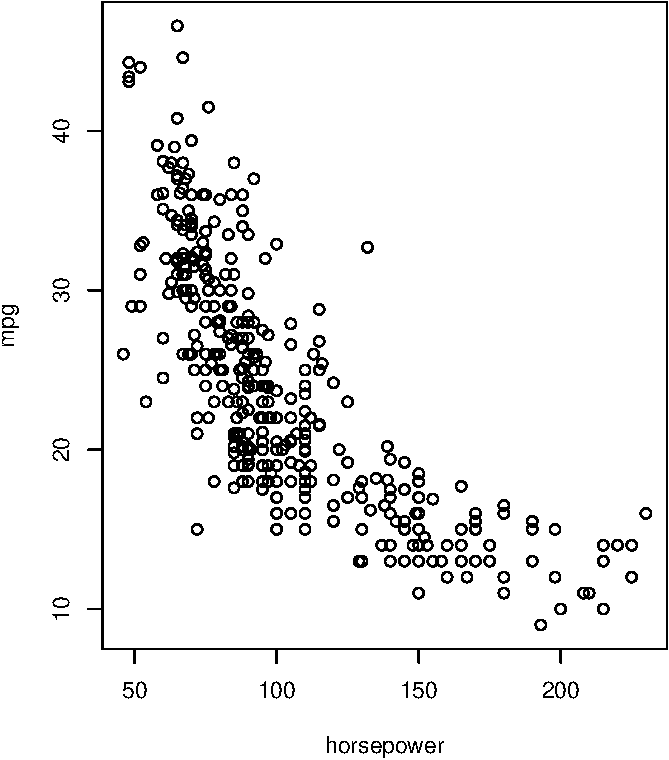
\includegraphics[width=1\linewidth]{JSS-article_files/figure-latex/mpg-horsepower-scatterplot-1} 

}

\caption[`mpg` vs `horsepower` for the `Auto` data]{`mpg` vs `horsepower` for the `Auto` data}\label{fig:mpg-horsepower-scatterplot}
\end{figure}
\end{CodeChunk}

The relationship between the two variables is monotone, decreasing, and
nonlinear. Following \citet{JamesEtAl:2021}, we'll consider
approximating the relationship by a polynomial regression, with the
degree of the polynomial \(p\) ranging from 1 (a linear regression) to
10.\footnote{Although it serves to illustrate the use of CV, a
  polynomial is probably not the best choice here. Consider, for example
  the scatterplot for log-transformed \texttt{mpg} and
  \texttt{horsepower}, produced by
  \texttt{plot(mpg\ \textasciitilde{}\ horsepower,\ data=Auto,\ log="xy")}
  (execution of which is left to the reader).} Polynomial fits for
\(p = 1\) to \(5\) are shown in the following figure:

\begin{CodeChunk}
\begin{CodeInput}
R> plot(mpg ~ horsepower, data=Auto)
R> horsepower <- with(Auto, 
+                    seq(min(horsepower), max(horsepower), 
+                        length=1000))
R> for (p in 1:5){
+   m <- lm(mpg ~ poly(horsepower,p), data=Auto)
+   mpg <- predict(m, newdata=data.frame(horsepower=horsepower))
+   lines(horsepower, mpg, col=p + 1, lty=p, lwd=2)
+ }
R> legend("topright", legend=1:5, col=2:6, lty=1:5, lwd=2,
+        title="Degree", inset=0.02)
\end{CodeInput}
\begin{figure}

{\centering 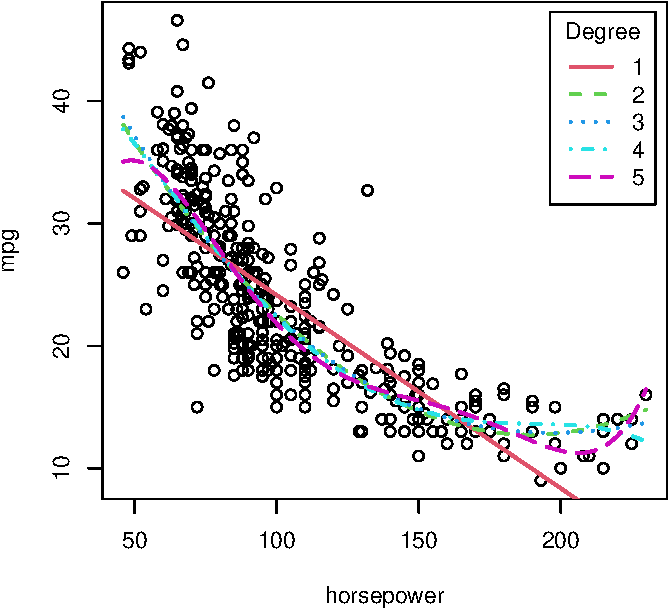
\includegraphics[width=1\linewidth]{JSS-article_files/figure-latex/mpg-horsepower-scatterplot-polynomials-1} 

}

\caption[`mpg` vs `horsepower` for the `Auto` data]{`mpg` vs `horsepower` for the `Auto` data}\label{fig:mpg-horsepower-scatterplot-polynomials}
\end{figure}
\end{CodeChunk}

The linear fit is clearly inappropriate; the fits for \(p = 2\)
(quadratic) through \(4\) are very similar; and the fit for \(p = 5\)
may over-fit the data by chasing one or two relatively high \texttt{mpg}
values at the right (but see the CV results reported below).

The following graph shows two measures of estimated (squared) error as a
function of polynomial-regression degree: The mean-squared error
(``MSE''), defined as
\(\mathsf{MSE} = \frac{1}{n}\sum_{i=1}^n (y_i - \widehat{y}_i)^2\), and
the usual residual variance, defined as
\(\widehat{\sigma}^2 = \frac{1}{n - p - 1} \sum_{i=1}^n (y_i - \widehat{y}_i)^2\).
The former necessarily declines with \(p\) (or, more strictly, can't
increase with \(p\)), while the latter gets slightly larger for the
largest values of \(p\), with the ``best'' value, by a small margin, for
\(p = 7\).

\begin{CodeChunk}
\begin{CodeInput}
R> library("cv") # for mse() and other functions
\end{CodeInput}
\begin{CodeOutput}
Loading required package: doParallel
\end{CodeOutput}
\begin{CodeOutput}
Loading required package: foreach
\end{CodeOutput}
\begin{CodeOutput}
Loading required package: iterators
\end{CodeOutput}
\begin{CodeOutput}
Loading required package: parallel
\end{CodeOutput}
\begin{CodeInput}
R> var <- mse <- numeric(10)
R> for (p in 1:10){
+   m <- lm(mpg ~ poly(horsepower, p), data=Auto)
+   mse[p] <- mse(Auto$mpg, fitted(m))
+   var[p] <- summary(m)$sigma^2
+ }
R> 
R> plot(c(1, 10), range(mse, var), type="n",
+      xlab="Degree of polynomial, p",
+      ylab="Estimated Squared Error")
R> lines(1:10, mse, lwd=2, lty=1, col=2, pch=16, type="b")
R> lines(1:10, var, lwd=2, lty=2, col=3, pch=17, type="b")
R> legend("topright", inset=0.02,
+        legend=c(expression(hat(sigma)^2), "MSE"),
+        lwd=2, lty=2:1, col=3:2, pch=17:16)
\end{CodeInput}
\begin{figure}

{\centering 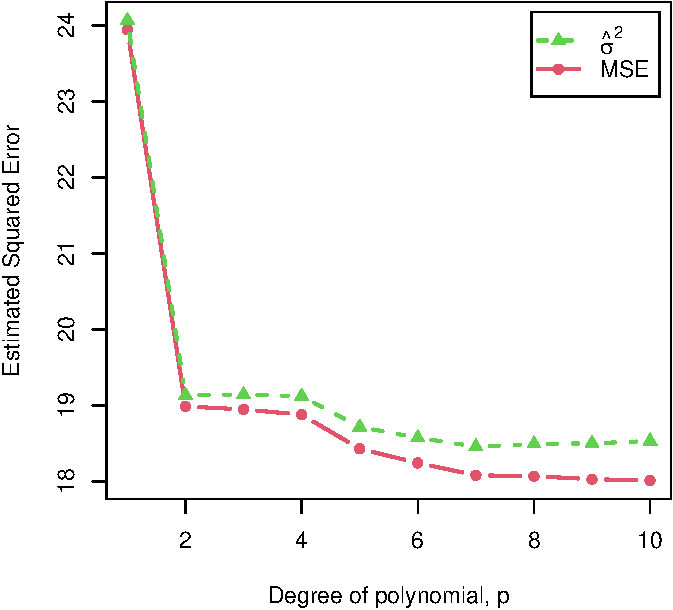
\includegraphics[width=1\linewidth]{JSS-article_files/figure-latex/mpg-horsepower-MSE-se-1} 

}

\caption[Estimated squared error as a function of polynomial degree, $p$]{Estimated squared error as a function of polynomial degree, $p$}\label{fig:mpg-horsepower-MSE-se}
\end{figure}
\end{CodeChunk}

The code for this graph uses the \texttt{mse()} function from the
\textbf{cv} package to compute the MSE for each fit.

\hypertarget{using-cv}{%
\subsubsection{Using cv()}\label{using-cv}}

The generic \texttt{cv()} function has an \texttt{"lm"} method, which by
default performs \(k = 10\)-fold CV:

\begin{CodeChunk}
\begin{CodeInput}
R> m.auto <- lm(mpg ~ poly(horsepower, 2), data=Auto)
R> summary(m.auto)
\end{CodeInput}
\begin{CodeOutput}

Call:
lm(formula = mpg ~ poly(horsepower, 2), data = Auto)

Residuals:
     Min       1Q   Median       3Q      Max 
-14.7135  -2.5943  -0.0859   2.2868  15.8961 

Coefficients:
                      Estimate Std. Error t value Pr(>|t|)
(Intercept)            23.4459     0.2209  106.13   <2e-16
poly(horsepower, 2)1 -120.1377     4.3739  -27.47   <2e-16
poly(horsepower, 2)2   44.0895     4.3739   10.08   <2e-16

Residual standard error: 4.374 on 389 degrees of freedom
Multiple R-squared:  0.6876,    Adjusted R-squared:  0.686 
F-statistic:   428 on 2 and 389 DF,  p-value: < 2.2e-16
\end{CodeOutput}
\begin{CodeInput}
R> cv(m.auto)
\end{CodeInput}
\begin{CodeOutput}
R RNG seed set to 534539
\end{CodeOutput}
\begin{CodeOutput}
10-Fold Cross Validation
method: Woodbury
criterion: mse
cross-validation criterion = 19.22944
bias-adjusted cross-validation criterion = 19.21651
full-sample criterion = 18.98477 
\end{CodeOutput}
\end{CodeChunk}

The \texttt{"lm"} method by default uses \texttt{mse()} as the CV
criterion and the Woodbury matrix identity to update the regression with
each fold deleted without having literally to refit the model.
Computational details are discussed in the final section of this
vignette. The function reports the CV estimate of MSE, a biased-adjusted
estimate of the MSE (the bias adjustment is explained in the final
section), and the MSE is also computed for the original, full-sample
regression. Because the division of the data into 10 folds is random,
\texttt{cv()} explicitly (randomly) generates and saves a seed for R's
pseudo-random number generator, to make the results replicable. The user
can also specify the seed directly via the \texttt{seed} argument to
\texttt{cv()}.

To perform LOO CV, we can set the \texttt{k} argument to \texttt{cv()}
to the number of cases in the data, here \texttt{k=392}, or, more
conveniently, to \texttt{k="loo"} or \texttt{k="n"}:

\begin{CodeChunk}
\begin{CodeInput}
R> cv(m.auto, k="loo")
\end{CodeInput}
\begin{CodeOutput}
n-Fold Cross Validation
method: hatvalues
criterion: mse
cross-validation criterion = 19.24821
\end{CodeOutput}
\end{CodeChunk}

For LOO CV of a linear model, \texttt{cv()} by default uses the
hatvalues from the model fit to the full data for the LOO updates, and
reports only the CV estimate of MSE. Alternative methods are to use the
Woodbury matrix identity or the ``naive'' approach of literally
refitting the model with each case omitted. All three methods produce
exact results for a linear model (within the precision of floating-point
computations):

\begin{CodeChunk}
\begin{CodeInput}
R> cv(m.auto, k="loo", method="naive")
\end{CodeInput}
\begin{CodeOutput}
n-Fold Cross Validation
method: naive
criterion: mse
cross-validation criterion = 19.24821
bias-adjusted cross-validation criterion = 19.24787
full-sample criterion = 18.98477 
\end{CodeOutput}
\begin{CodeInput}
R> cv(m.auto, k="loo", method="Woodbury")
\end{CodeInput}
\begin{CodeOutput}
n-Fold Cross Validation
method: Woodbury
criterion: mse
cross-validation criterion = 19.24821
bias-adjusted cross-validation criterion = 19.24787
full-sample criterion = 18.98477 
\end{CodeOutput}
\end{CodeChunk}

The \texttt{"naive"} and \texttt{"Woodbury"} methods also return the
bias-adjusted estimate of MSE and the full-sample MSE, but bias isn't an
issue for LOO CV.

This is a small regression problem and all three computational
approaches are essentially instantaneous, but it is still of interest to
investigate their relative speed. In this comparison, we include the
\texttt{cv.glm()} function from the \textbf{boot} package, which takes
the naive approach, and for which we have to fit the linear model as an
equivalent Gaussian GLM. We use the \texttt{microbenchmark()} function
from the package of the same name for the timings \citep{Mersmann:2023}:

\begin{CodeChunk}
\begin{CodeInput}
R> m.auto.glm <- glm(mpg ~ poly(horsepower, 2), data=Auto)
R> boot::cv.glm(Auto, m.auto.glm)$delta
\end{CodeInput}
\begin{CodeOutput}
[1] 19.24821 19.24787
\end{CodeOutput}
\begin{CodeInput}
R> microbenchmark::microbenchmark(
+   hatvalues = cv(m.auto, k="loo"),
+   Woodbury = cv(m.auto, k="loo", method="Woodbury"),
+   naive = cv(m.auto, k="loo", method="naive"),
+   cv.glm = boot::cv.glm(Auto, m.auto.glm),
+   times=10
+ )
\end{CodeInput}
\begin{CodeOutput}
Warning in microbenchmark::microbenchmark(hatvalues = cv(m.auto, k = "loo"), :
less accurate nanosecond times to avoid potential integer overflows
\end{CodeOutput}
\begin{CodeOutput}
Unit: microseconds
      expr        min        lq       mean     median         uq        max
 hatvalues    977.973    993.43   1143.433   1173.113   1202.981   1296.256
  Woodbury   9932.004  10178.21  11461.993  10363.201  10865.943  17762.266
     naive 215384.152 217809.02 224546.766 219116.505 221670.231 275518.278
    cv.glm 384357.616 388159.59 409612.546 390652.100 441741.913 443226.605
 neval cld
    10 a  
    10 a  
    10  b 
    10   c
\end{CodeOutput}
\end{CodeChunk}

On our computer, using the hatvalues is about an order of magnitude
faster than employing Woodbury matrix updates, and more than two orders
of magnitude faster than refitting the model.\footnote{Out of
  impatience, we asked \texttt{microbenchmark()} to execute each command
  only 10 times rather than the default 100. With the exception of the
  last columns, the output is self-explanatory. The last column shows
  which methods have average timings that are statistically
  distinguishable. Because of the small number of repetitions (i.e.,
  10), the \texttt{"hatvalues"} and \texttt{"Woodbury"} methods aren't
  distinguishable, but the difference between these methods persists
  when we perform more repetitions---we invite the reader to redo this
  computation with the default \texttt{times=100} repetitions.}

\hypertarget{comparing-competing-models}{%
\subsubsection{Comparing competing
models}\label{comparing-competing-models}}

The \texttt{cv()} function also has a method that can be applied to a
list of regression models for the same data, composed using the
\texttt{models()} function. For \(k\)-fold CV, the same folds are used
for the competing models, which reduces random error in their
comparison. This result can also be obtained by specifying a common seed
for R's random-number generator while applying \texttt{cv()} separately
to each model, but employing a list of models is more convenient for
both \(k\)-fold and LOO CV (where there is no random component to the
composition of the \(n\) folds).

We illustrate with the polynomial regression models of varying degree
for the \texttt{Auto} data (discussed previously), beginning by fitting
and saving the 10 models:

\begin{CodeChunk}
\begin{CodeInput}
R> for (p in 1:10){
+   assign(paste0("m.", p),
+          lm(mpg ~ poly(horsepower, p), data=Auto))
+ }
R> objects(pattern="m\\.[0-9]")
\end{CodeInput}
\begin{CodeOutput}
 [1] "m.1"  "m.10" "m.2"  "m.3"  "m.4"  "m.5"  "m.6"  "m.7"  "m.8"  "m.9" 
\end{CodeOutput}
\begin{CodeInput}
R> summary(m.2) # for example, the quadratic fit
\end{CodeInput}
\begin{CodeOutput}

Call:
lm(formula = mpg ~ poly(horsepower, p), data = Auto)

Residuals:
     Min       1Q   Median       3Q      Max 
-14.7135  -2.5943  -0.0859   2.2868  15.8961 

Coefficients:
                      Estimate Std. Error t value Pr(>|t|)
(Intercept)            23.4459     0.2209  106.13   <2e-16
poly(horsepower, p)1 -120.1377     4.3739  -27.47   <2e-16
poly(horsepower, p)2   44.0895     4.3739   10.08   <2e-16

Residual standard error: 4.374 on 389 degrees of freedom
Multiple R-squared:  0.6876,    Adjusted R-squared:  0.686 
F-statistic:   428 on 2 and 389 DF,  p-value: < 2.2e-16
\end{CodeOutput}
\end{CodeChunk}

We then apply \texttt{cv()} to the list of 10 models (the \texttt{data}
argument is required):

\begin{CodeChunk}
\begin{CodeInput}
R> # 10-fold CV
R> cv.auto.10 <- cv(models(m.1, m.2, m.3, m.4, m.5,
+                      m.6, m.7, m.8, m.9, m.10),
+               data=Auto, seed=2120)
R> cv.auto.10[1:2] # for the linear and quadratic models
\end{CodeInput}
\begin{CodeOutput}

Model model.1:
10-Fold Cross Validation
method: Woodbury
cross-validation criterion = 24.24642
bias-adjusted cross-validation criterion = 24.23039
full-sample criterion = 23.94366 

Model model.2:
10-Fold Cross Validation
method: Woodbury
cross-validation criterion = 19.34601
bias-adjusted cross-validation criterion = 19.32699
full-sample criterion = 18.98477 
\end{CodeOutput}
\begin{CodeInput}
R> # LOO CV
R> cv.auto.loo <- cv(models(m.1, m.2, m.3, m.4, m.5,
+                         m.6, m.7, m.8, m.9, m.10),
+                  data=Auto, k="loo")
R> cv.auto.loo[1:2] # linear and quadratic models
\end{CodeInput}
\begin{CodeOutput}

Model model.1:
n-Fold Cross Validation
method: hatvalues
cross-validation criterion = 24.23151
Model model.2:
n-Fold Cross Validation
method: hatvalues
cross-validation criterion = 19.24821
\end{CodeOutput}
\end{CodeChunk}

Because we didn't supply names for the models in the calls to the
\texttt{models()} function, the names \texttt{model.1},
\texttt{model.2}, etc., are generated by the function.

Finally, we extract and graph the adjusted MSEs for \(10\)-fold CV and
the MSEs for LOO CV:

\begin{CodeChunk}
\begin{CodeInput}
R> cv.mse.10 <- sapply(cv.auto.10, function(x) x[["adj CV crit"]])
R> cv.mse.loo <- sapply(cv.auto.loo, function(x) x[["CV crit"]])
R> plot(c(1, 10), range(cv.mse.10, cv.mse.loo), type="n",
+      xlab="Degree of polynomial, p",
+      ylab="Cross-Validated MSE")
R> lines(1:10, cv.mse.10, lwd=2, lty=1, col=2, pch=16, type="b")
R> lines(1:10, cv.mse.loo, lwd=2, lty=2, col=3, pch=17, type="b")
R> legend("topright", inset=0.02,
+        legend=c("10-Fold CV", "LOO CV"),
+        lwd=2, lty=2:1, col=3:2, pch=17:16)
\end{CodeInput}
\begin{figure}

{\centering 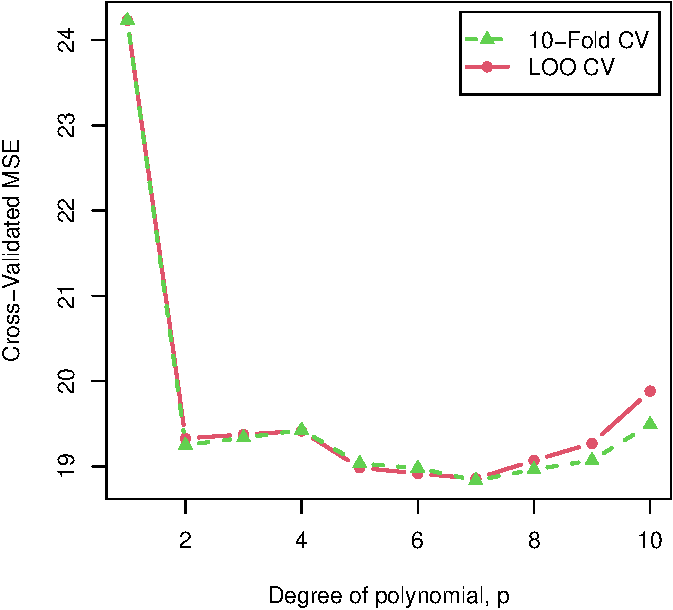
\includegraphics[width=1\linewidth]{JSS-article_files/figure-latex/polynomial-regression-CV-graph-1} 

}

\caption[Cross-validated 10-fold and LOO MSE as a function of polynomial degree, $p$]{Cross-validated 10-fold and LOO MSE as a function of polynomial degree, $p$}\label{fig:polynomial-regression-CV-graph}
\end{figure}
\end{CodeChunk}

Alternatively, we can use the \texttt{plot()} method for
\texttt{"cvModList"} objects to compare the models, though with separate
graphs for 10-fold and LOO CV:

\begin{CodeChunk}
\begin{CodeInput}
R> plot(cv.auto.10, main="Polynomial Regressions, 10-Fold CV",
+      axis.args=list(labels=1:10), xlab="Degree of Polynomial, p")
R> plot(cv.auto.loo, main="Polynomial Regressions, LOO CV",
+      axis.args=list(labels=1:10), xlab="Degree of Polynomial, p")
\end{CodeInput}
\begin{figure}

{\centering 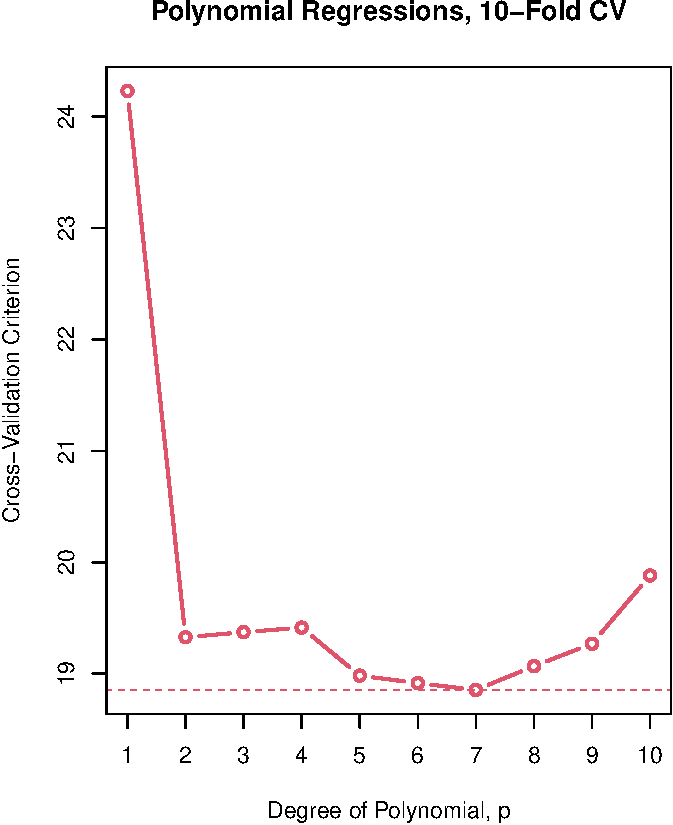
\includegraphics[width=0.45\linewidth]{JSS-article_files/figure-latex/polynomial-regression-CV-graph-2-1} 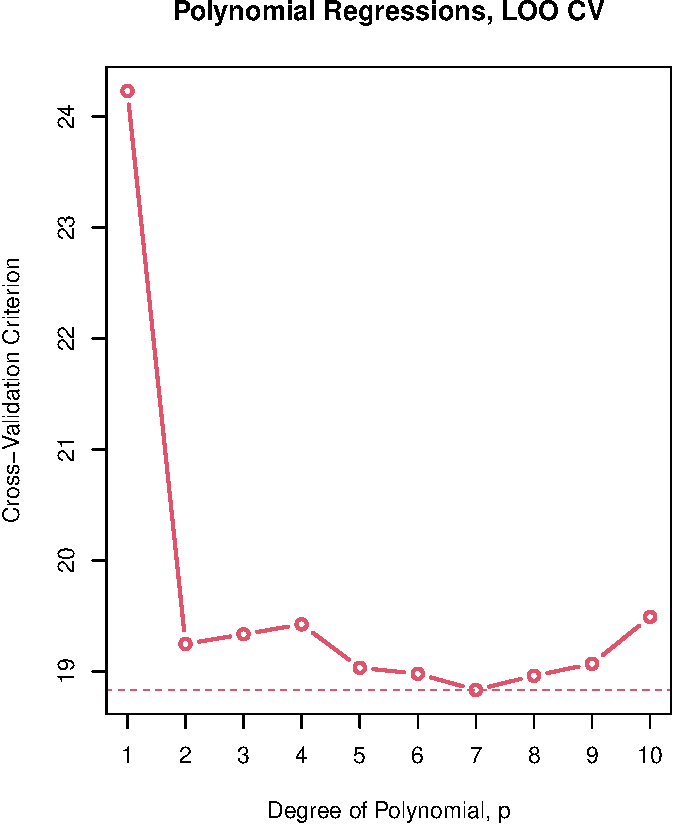
\includegraphics[width=0.45\linewidth]{JSS-article_files/figure-latex/polynomial-regression-CV-graph-2-2} 

}

\caption[Cross-validated 10-fold and LOO MSE as a function of polynomial degree, $p$]{Cross-validated 10-fold and LOO MSE as a function of polynomial degree, $p$}\label{fig:polynomial-regression-CV-graph-2}
\end{figure}
\end{CodeChunk}

In this example, 10-fold and LOO CV produce generally similar results,
and also results that are similar to those produced by the estimated
error variance \(\widehat{\sigma}^2\) for each model, reported above
(except for the highest-degree polynomials, where the CV results more
clearly suggest over-fitting).

\hypertarget{logistic-regression-for-the-mroz-data}{%
\subsection{Logistic regression for the Mroz
data}\label{logistic-regression-for-the-mroz-data}}

The \texttt{Mroz} data set from the \textbf{carData} package
\citep[associated with][]{FoxWeisberg:2019} has been used by several
authors to illustrate binary logistic regression; see, in particular
\citet{FoxWeisberg:2019}. The data were originally drawn from the U.S.
Panel Study of Income Dynamics and pertain to married women. Here are a
few cases in the data set:

\begin{CodeChunk}
\begin{CodeInput}
R> data("Mroz", package="carData")
R> head(Mroz, 3)
\end{CodeInput}
\begin{CodeOutput}
  lfp k5 k618 age wc hc       lwg   inc
1 yes  1    0  32 no no 1.2101647 10.91
2 yes  0    2  30 no no 0.3285041 19.50
3 yes  1    3  35 no no 1.5141279 12.04
\end{CodeOutput}
\begin{CodeInput}
R> tail(Mroz, 3)
\end{CodeInput}
\begin{CodeOutput}
    lfp k5 k618 age wc hc       lwg    inc
751  no  0    0  43 no no 0.8881401  9.952
752  no  0    0  60 no no 1.2249736 24.984
753  no  0    3  39 no no 0.8532125 28.363
\end{CodeOutput}
\end{CodeChunk}

The response variable in the logistic regression is \texttt{lfp},
labor-force participation, a factor coded \texttt{"yes"} or
\texttt{"no"}. The remaining variables are predictors:

\begin{itemize}
\tightlist
\item
  \texttt{k5}, number of children 5 years old of younger in the woman's
  household;
\item
  \texttt{k618}, number of children between 6 and 18 years old;
\item
  \texttt{age}, in years;
\item
  \texttt{wc}, wife's college attendance, \texttt{"yes"} or
  \texttt{"no"};
\item
  \texttt{hc}, husband's college attendance;
\item
  \texttt{lwg}, the woman's log wage rate if she is employed, or her
  \emph{imputed} wage rate, if she is not \citep[a variable that][ show
  is problematically defined]{FoxWeisberg:2019}; and
\item
  \texttt{inc}, family income, in \$1000s, exclusive of wife's income.
\end{itemize}

We use the \texttt{glm()} function to fit a binary logistic regression
to the \texttt{Mroz} data:

\begin{CodeChunk}
\begin{CodeInput}
R> m.mroz <- glm(lfp ~ ., data=Mroz, family=binomial)
R> summary(m.mroz)
\end{CodeInput}
\begin{CodeOutput}

Call:
glm(formula = lfp ~ ., family = binomial, data = Mroz)

Coefficients:
             Estimate Std. Error z value Pr(>|z|)
(Intercept)  3.182140   0.644375   4.938 7.88e-07
k5          -1.462913   0.197001  -7.426 1.12e-13
k618        -0.064571   0.068001  -0.950 0.342337
age         -0.062871   0.012783  -4.918 8.73e-07
wcyes        0.807274   0.229980   3.510 0.000448
hcyes        0.111734   0.206040   0.542 0.587618
lwg          0.604693   0.150818   4.009 6.09e-05
inc         -0.034446   0.008208  -4.196 2.71e-05

(Dispersion parameter for binomial family taken to be 1)

    Null deviance: 1029.75  on 752  degrees of freedom
Residual deviance:  905.27  on 745  degrees of freedom
AIC: 921.27

Number of Fisher Scoring iterations: 4
\end{CodeOutput}
\begin{CodeInput}
R> BayesRule(ifelse(Mroz$lfp == "yes", 1, 0), 
+           fitted(m.mroz, type="response"))
\end{CodeInput}
\begin{CodeOutput}
[1] 0.3067729
attr(,"casewise loss")
[1] "y != round(yhat)"
\end{CodeOutput}
\end{CodeChunk}

In addition to the usually summary output for a GLM, we show the result
of applying the \texttt{BayesRule()} function from the \textbf{cv}
package to predictions derived from the fitted model. Bayes rule, which
predicts a ``success'' in a binary regression model when the fitted
probability of success {[}i.e., \(\phi = \Pr(y = 1)\){]} is
\(\widehat{\phi} \ge .5\) and a ``failure'' if
\(\widehat{\phi} < .5\).\footnote{\texttt{BayesRule()} does some error
  checking; \texttt{BayesRule2()} is similar, but omits the error
  checking, and so can be faster for large problems.} The first argument
to \texttt{BayesRule()} is the binary \{0, 1\} response, and the second
argument is the predicted probability of success. \texttt{BayesRule()}
returns the proportion of predictions that are \emph{in error}, as
appropriate for a ``cost'' function.

The value returned by \texttt{BayesRule()} is associated with an
``attribute'' named \texttt{"casewise\ loss"} and set to
\texttt{"y\ !=\ round(yhat)"}, signifying that the Bayes rule CV
criterion is computed as the mean of casewise values, here 0 if the
prediction for a case matches the observed value and 1 if it does not
(signifying a prediction error). The \texttt{mse()} function for numeric
responses is also calculated as a casewise average. Some other criteria,
such as the median absolute error, computed by the \texttt{medAbsErr()}
function in the \textbf{cv} package, aren't averages of casewise
components. The distinction is important because, to our knowledge, the
statistical theory of cross-validation, for example, in
\citet{DavisonHinkley:1997}, \citet{BatesHastieTibshirani:2023}, and
\citet{ArlotCelisse:2010}, is developed for CV criteria like MSE that
are means of casewise components. As a consequence, we limit computation
of bias adjustment and confidence intervals (see below) to criteria that
are casewise averages.

In this example, the fitted logistic regression incorrectly predicts
31\% of the responses; we expect this estimate to be optimistic given
that the model is used to ``predict'' the data to which it is fit.

The \texttt{"glm"} method for \texttt{cv()} is largely similar to the
\texttt{"lm"} method, although the default algorithm, selected
explicitly by \texttt{method="exact"}, refits the model with each fold
removed (and is thus equivalent to \texttt{method="naive"} for
\texttt{"lm"} models). For generalized linear models,
\texttt{method="Woodbury"} or (for LOO CV) \texttt{method="hatvalues"}
provide approximate results (see the last section of the vignette for
details):

\begin{CodeChunk}
\begin{CodeInput}
R> cv(m.mroz, criterion=BayesRule, seed=248)
\end{CodeInput}
\begin{CodeOutput}
R RNG seed set to 248
\end{CodeOutput}
\begin{CodeOutput}
10-Fold Cross Validation
method: exact
criterion: BayesRule
cross-validation criterion = 0.3240372
bias-adjusted cross-validation criterion = 0.3195223
95% CI for bias-adjusted CV criterion = (0.2860721, 0.3529724)
full-sample criterion = 0.3067729 
\end{CodeOutput}
\begin{CodeInput}
R> cv(m.mroz, criterion=BayesRule, seed=248, method="Woodbury")
\end{CodeInput}
\begin{CodeOutput}
R RNG seed set to 248
\end{CodeOutput}
\begin{CodeOutput}
10-Fold Cross Validation
method: Woodbury
criterion: BayesRule
cross-validation criterion = 0.3240372
bias-adjusted cross-validation criterion = 0.3192577
95% CI for bias-adjusted CV criterion = (0.2858076, 0.3527079)
full-sample criterion = 0.3067729 
\end{CodeOutput}
\end{CodeChunk}

To ensure that the two methods use the same 10 folds, we specify the
seed for R's random-number generator explicitly; here, and as is common
in our experience, the \texttt{"exact"} and \texttt{"Woodbury"}
algorithms produce nearly identical results. The CV estimates of
prediction error are slightly higher than the estimate based on all of
the cases.

The printed output includes a 95\% confidence interval for the
bias-adjusted Bayes rule CV criterion.
\citet{BatesHastieTibshirani:2023} show that these confidence intervals
are unreliable for models fit to small samples, and by default
\texttt{cv()} computes them only when the sample size is 400 or larger
and when the CV criterion employed is an average of casewise components,
as is the case for Bayes rule. See the final section of the vignette for
details of the computation of confidence intervals for bias-adjusted CV
criteria.

Here are results of applying LOO CV to the Mroz model, using both the
exact and the approximate methods:

\begin{CodeChunk}
\begin{CodeInput}
R> cv(m.mroz, k="loo", criterion=BayesRule)
\end{CodeInput}
\begin{CodeOutput}
n-Fold Cross Validation
method: exact
criterion: BayesRule
cross-validation criterion = 0.3200531
bias-adjusted cross-validation criterion = 0.3183001
95% CI for bias-adjusted CV criterion = (0.2849584, 0.3516418)
full-sample criterion = 0.3067729 
\end{CodeOutput}
\begin{CodeInput}
R> cv(m.mroz, k="loo", criterion=BayesRule, method="Woodbury")
\end{CodeInput}
\begin{CodeOutput}
n-Fold Cross Validation
method: Woodbury
criterion: BayesRule
cross-validation criterion = 0.3200531
bias-adjusted cross-validation criterion = 0.3183001
95% CI for bias-adjusted CV criterion = (0.2849584, 0.3516418)
full-sample criterion = 0.3067729 
\end{CodeOutput}
\begin{CodeInput}
R> cv(m.mroz, k="loo", criterion=BayesRule, method="hatvalues")
\end{CodeInput}
\begin{CodeOutput}
n-Fold Cross Validation
method: hatvalues
criterion: BayesRule
cross-validation criterion = 0.3200531
\end{CodeOutput}
\end{CodeChunk}

To the number of decimal digits shown, the three methods produce
identical results for this example.

As for linear models, we report some timings for the various
\texttt{cv()} methods of computation in LOO CV as well as for the
\texttt{cv.glm()} function from the \textbf{boot} package (which,
recall, refits the model with each case removed, and thus is comparable
to \texttt{cv()} with \texttt{method="exact"}):

\begin{CodeChunk}
\begin{CodeInput}
R> microbenchmark::microbenchmark(
+   hatvalues=cv(m.mroz, k="loo", criterion=BayesRule, method="hatvalues"),
+   Woodbury=cv(m.mroz, k="loo", criterion=BayesRule, method="Woodbury"),
+   exact=cv(m.mroz, k="loo", criterion=BayesRule),
+   cv.glm=boot::cv.glm(Mroz, m.mroz,
+                cost=BayesRule),
+   times=10)
\end{CodeInput}
\begin{CodeOutput}
Unit: milliseconds
      expr         min          lq        mean      median          uq
 hatvalues    1.316141    1.326842    1.654063    1.407571    1.442462
  Woodbury   37.127427   38.641639   39.368192   39.356904   40.562202
     exact 1757.625925 1827.861385 1905.072191 1911.421128 1951.049944
    cv.glm 2062.693354 2122.649130 2149.761134 2140.079440 2184.788525
         max neval cld
    4.022428    10 a  
   41.060188    10 a  
 2128.307540    10  b 
 2299.544573    10   c
\end{CodeOutput}
\end{CodeChunk}

There is a substantial time penalty associated with exact computations.

\hypertarget{cross-validating-mixed-effects-models}{%
\section{Cross-validating mixed-effects
models}\label{cross-validating-mixed-effects-models}}

The fundamental analogy for cross-validation is to the collection of new
data. That is, predicting the response in each fold from the model fit
to data in the other folds is like using the model fit to all of the
data to predict the response for new cases from the values of the
predictors for those new cases. As we explained, the application of this
idea to independently sampled cases is straightforward---simply
partition the data into random folds of equal size and leave each fold
out in turn, or, in the case of LOO CV, simply omit each case in turn.

In contrast, mixed-effects models are fit to \emph{dependent} data, in
which cases as clustered, such as hierarchical data, where the clusters
comprise higher-level units (e.g., students clustered in schools), or
longitudinal data, where the clusters are individuals and the cases
repeated observations on the individuals over time.\footnote{There are,
  however, more complex situations that give rise to so-called
  \emph{crossed} (rather than \emph{nested}) random effects. For
  example, consider students within classes within schools. In primary
  schools, students typically are in a single class, and so classes are
  nested within schools. In secondary schools, however, students
  typically take several classes and students who are together in a
  particular class may not be together in other classes; consequently,
  random effects based on classes within schools are crossed. The
  \texttt{lmer()} function in the \textbf{lme4} package is capable of
  modeling both nested and crossed random effects, and the \texttt{cv()}
  methods for mixed models in the \textbf{cv} package pertain to both
  nested and crossed random effects. We present an example of the latter
  later in the vignette.}

We can think of two approaches to applying cross-validation to clustered
data:\footnote{We subsequently discovered that \citet[Section
  8]{Vehtari:2023} makes similar points.}

\begin{enumerate}
\def\labelenumi{\arabic{enumi}.}
\item
  Treat CV as analogous to predicting the response for one or more cases
  in a \emph{newly observed cluster}. In this instance, the folds
  comprise one or more whole clusters; we refit the model with all of
  the cases in clusters in the current fold removed; and then we predict
  the response for the cases in clusters in the current fold. These
  predictions are based only on fixed effects because the random effects
  for the omitted clusters are presumably unknown, as they would be for
  data on cases in newly observed clusters.
\item
  Treat CV as analogous to predicting the response for a newly observed
  case in an \emph{existing cluster}. In this instance, the folds
  comprise one or more individual cases, and the predictions can use
  both the fixed and random effects.
\end{enumerate}

\hypertarget{example-the-high-school-and-beyond-data}{%
\subsection{Example: The High-School and Beyond
data}\label{example-the-high-school-and-beyond-data}}

Following their use by \citet{RaudenbushBryk:2002}, data from the 1982
\emph{High School and Beyond} (HSB) survey have become a staple of the
literature on mixed-effects models. The HSB data are used by \citet[Sec.
7.2.2]{FoxWeisberg:2019} to illustrate the application of linear mixed
models to hierarchical data, and we'll closely follow their example
here.

The HSB data are included in the \texttt{MathAchieve} and
\texttt{MathAchSchool} data sets in the \textbf{nlme} package
\citep{PinheiroBates:2000}. \texttt{MathAchieve} includes
individual-level data on 7185 students in 160 high schools, and
\texttt{MathAchSchool} includes school-level data:

\begin{CodeChunk}
\begin{CodeInput}
R> data("MathAchieve", package="nlme")
R> dim(MathAchieve)
\end{CodeInput}
\begin{CodeOutput}
[1] 7185    6
\end{CodeOutput}
\begin{CodeInput}
R> head(MathAchieve, 3)
\end{CodeInput}
\begin{CodeOutput}
Grouped Data: MathAch ~ SES | School
  School Minority    Sex    SES MathAch MEANSES
1   1224       No Female -1.528   5.876  -0.428
2   1224       No Female -0.588  19.708  -0.428
3   1224       No   Male -0.528  20.349  -0.428
\end{CodeOutput}
\begin{CodeInput}
R> tail(MathAchieve, 3)
\end{CodeInput}
\begin{CodeOutput}
Grouped Data: MathAch ~ SES | School
     School Minority    Sex    SES MathAch MEANSES
7183   9586       No Female  1.332  19.641   0.627
7184   9586       No Female -0.008  16.241   0.627
7185   9586       No Female  0.792  22.733   0.627
\end{CodeOutput}
\begin{CodeInput}
R> data("MathAchSchool", package="nlme")
R> dim(MathAchSchool)
\end{CodeInput}
\begin{CodeOutput}
[1] 160   7
\end{CodeOutput}
\begin{CodeInput}
R> head(MathAchSchool, 2)
\end{CodeInput}
\begin{CodeOutput}
     School Size Sector PRACAD DISCLIM HIMINTY MEANSES
1224   1224  842 Public   0.35   1.597       0  -0.428
1288   1288 1855 Public   0.27   0.174       0   0.128
\end{CodeOutput}
\begin{CodeInput}
R> tail(MathAchSchool, 2)
\end{CodeInput}
\begin{CodeOutput}
     School Size   Sector PRACAD DISCLIM HIMINTY MEANSES
9550   9550 1532   Public   0.45   0.791       0   0.059
9586   9586  262 Catholic   1.00  -2.416       0   0.627
\end{CodeOutput}
\end{CodeChunk}

The first few students are in school number 1224 and the last few in
school 9586.

We'll use only the \texttt{School}, \texttt{SES} (students'
socioeconomic status), and \texttt{MathAch} (their score on a
standardized math-achievement test) variables in the
\texttt{MathAchieve} data set, and \texttt{Sector} (\texttt{"Catholic"}
or \texttt{"Public"}) in the \texttt{MathAchSchool} data set.

Some data-management is required before fitting a mixed-effects model to
the HSB data, for which we use the \textbf{dplyr} package
\citep{WickhamEtAl:2023}:

\begin{CodeChunk}
\begin{CodeInput}
R> library("dplyr")
\end{CodeInput}
\begin{CodeOutput}

Attaching package: 'dplyr'
\end{CodeOutput}
\begin{CodeOutput}
The following objects are masked from 'package:stats':

    filter, lag
\end{CodeOutput}
\begin{CodeOutput}
The following objects are masked from 'package:base':

    intersect, setdiff, setequal, union
\end{CodeOutput}
\begin{CodeInput}
R> MathAchieve %>% group_by(School) %>%
+   summarize(mean.ses = mean(SES)) -> Temp
R> Temp <- merge(MathAchSchool, Temp, by="School")
R> HSB <- merge(Temp[, c("School", "Sector", "mean.ses")],
+              MathAchieve[, c("School", "SES", "MathAch")], by="School")
R> names(HSB) <- tolower(names(HSB))
R> 
R> HSB$cses <- with(HSB, ses - mean.ses)
\end{CodeInput}
\end{CodeChunk}

In the process, we created two new school-level variables:
\texttt{meanses}, which is the average SES for students in each school;
and \texttt{cses}, which is school-average SES centered at its mean. For
details, see \citet[Sec. 7.2.2]{FoxWeisberg:2019}.

Still following Fox and Weisberg, we proceed to use the \texttt{lmer()}
function in the \textbf{lme4} package \citep{BatesEtAl:2015} to fit a
mixed model for math achievement to the HSB data:

\begin{CodeChunk}
\begin{CodeInput}
R> library("lme4")
\end{CodeInput}
\begin{CodeOutput}
Loading required package: Matrix
\end{CodeOutput}
\begin{CodeInput}
R> hsb.lmer <- lmer(mathach ~ mean.ses*cses + sector*cses
+                    + (cses | school), data=HSB)
R> summary(hsb.lmer, correlation=FALSE)
\end{CodeInput}
\begin{CodeOutput}
Linear mixed model fit by REML ['lmerMod']
Formula: mathach ~ mean.ses * cses + sector * cses + (cses | school)
   Data: HSB

REML criterion at convergence: 46503.7

Scaled residuals: 
     Min       1Q   Median       3Q      Max 
-3.15926 -0.72319  0.01704  0.75444  2.95822 

Random effects:
 Groups   Name        Variance Std.Dev. Corr
 school   (Intercept)  2.380   1.5426       
          cses         0.101   0.3179   0.39
 Residual             36.721   6.0598       
Number of obs: 7185, groups:  school, 160

Fixed effects:
                    Estimate Std. Error t value
(Intercept)          12.1279     0.1993  60.856
mean.ses              5.3329     0.3692  14.446
cses                  2.9450     0.1556  18.928
sectorCatholic        1.2266     0.3063   4.005
mean.ses:cses         1.0393     0.2989   3.477
cses:sectorCatholic  -1.6427     0.2398  -6.851
\end{CodeOutput}
\end{CodeChunk}

We can then cross-validate at the cluster (i.e., school) level,

\begin{CodeChunk}
\begin{CodeInput}
R> cv(hsb.lmer, k=10, clusterVariables="school", seed=5240)
\end{CodeInput}
\begin{CodeOutput}
R RNG seed set to 5240
\end{CodeOutput}
\begin{CodeOutput}
10-Fold Cross Validation based on 160 {school} clusters
cross-validation criterion = 39.15662
bias-adjusted cross-validation criterion = 39.14844
95% CI for bias-adjusted CV criterion = (38.06554, 40.23135)
full-sample criterion = 39.00599 
\end{CodeOutput}
\end{CodeChunk}

or at the case (i.e., student) level,

\begin{CodeChunk}
\begin{CodeInput}
R> cv(hsb.lmer, seed=1575)
\end{CodeInput}
\begin{CodeOutput}
R RNG seed set to 1575
\end{CodeOutput}
\begin{CodeOutput}
Warning in checkConv(attr(opt, "derivs"), opt$par, ctrl = control$checkConv, :
Model failed to converge with max|grad| = 0.00587228 (tol = 0.002, component 1)
\end{CodeOutput}
\begin{CodeOutput}
boundary (singular) fit: see help('isSingular')
\end{CodeOutput}
\begin{CodeOutput}
10-Fold Cross Validation
cross-validation criterion = 37.44473
bias-adjusted cross-validation criterion = 37.33801
95% CI for bias-adjusted CV criterion = (36.28761, 38.38841)
full-sample criterion = 36.06767 
\end{CodeOutput}
\end{CodeChunk}

For cluster-level CV, the \texttt{clusterVariables} argument tells
\texttt{cv()} how the clusters are defined. Were there more than one
clustering variable, say classes within schools, these would be provided
as a character vector of variable names:
\texttt{clusterVariables\ =\ c("school",\ "class")}. For cluster-level
CV, the default is \texttt{k\ =\ "loo"}, that is, leave one cluster out
at a time; we instead specify \texttt{k\ =\ 10} folds of clusters, each
fold therefore comprising \(160/10 = 16\) schools.

If the \texttt{clusterVariables} argument is omitted, then case-level CV
is employed, with \texttt{k\ =\ 10} folds as the default, here each with
\(7185/10 \approx 719\) students. Notice that one of the 10 models refit
with a fold removed failed to converge. Convergence problems are common
in mixed-effects modeling. The apparent issue here is that an estimated
variance component is close to or equal to 0, which is at a boundary of
the parameter space. That shouldn't disqualify the fitted model for the
kind of prediction required for cross-validation.

There is also a \texttt{cv()} method for linear mixed models fit by the
\texttt{lme()} function in the \textbf{nlme} package, and the arguments
for \texttt{cv()} in this case are the same as for a model fit by
\texttt{lmer()} or \texttt{glmer()}. We illustrate with the mixed model
fit to the HSB data:

\begin{CodeChunk}
\begin{CodeInput}
R> library(nlme)
R> hsb.lme <- lme(mathach ~ mean.ses*cses + sector*cses,
+                  random = ~ cses | school, data=HSB,
+                control=list(opt="optim"))
R> summary(hsb.lme)
\end{CodeInput}
\begin{CodeOutput}
Linear mixed-effects model fit by REML
  Data: HSB 
       AIC      BIC    logLik
  46524.78 46593.57 -23252.39

Random effects:
 Formula: ~cses | school
 Structure: General positive-definite, Log-Cholesky parametrization
            StdDev     Corr  
(Intercept) 1.54117685 (Intr)
cses        0.01817364 0.006 
Residual    6.06349216       

Fixed effects:  mathach ~ mean.ses * cses + sector * cses 
                        Value Std.Error   DF  t-value p-value
(Intercept)         12.128207 0.1991964 7022 60.88567   0e+00
mean.ses             5.336665 0.3689784  157 14.46335   0e+00
cses                 2.942145 0.1512240 7022 19.45554   0e+00
sectorCatholic       1.224531 0.3061139  157  4.00025   1e-04
mean.ses:cses        1.044406 0.2910747 7022  3.58810   3e-04
cses:sectorCatholic -1.642148 0.2331162 7022 -7.04433   0e+00
 Correlation: 
                    (Intr) men.ss cses   sctrCt mn.ss:
mean.ses             0.256                            
cses                 0.000  0.000                     
sectorCatholic      -0.699 -0.356  0.000              
mean.ses:cses        0.000  0.000  0.295  0.000       
cses:sectorCatholic  0.000  0.000 -0.696  0.000 -0.351

Standardized Within-Group Residuals:
        Min          Q1         Med          Q3         Max 
-3.17010624 -0.72487654  0.01489162  0.75426269  2.96549829 

Number of Observations: 7185
Number of Groups: 160 
\end{CodeOutput}
\begin{CodeInput}
R> cv(hsb.lme, k=10, clusterVariables="school", seed=5240)
\end{CodeInput}
\begin{CodeOutput}
R RNG seed set to 5240
\end{CodeOutput}
\begin{CodeOutput}
10-Fold Cross Validation based on 160 {school} clusters
cross-validation criterion = 39.1569
bias-adjusted cross-validation criterion = 39.14881
95% CI for bias-adjusted CV criterion = (38.06591, 40.23171)
full-sample criterion = 39.0062 
\end{CodeOutput}
\begin{CodeInput}
R> cv(hsb.lme, seed=1575)
\end{CodeInput}
\begin{CodeOutput}
R RNG seed set to 1575
\end{CodeOutput}
\begin{CodeOutput}
10-Fold Cross Validation
cross-validation criterion = 37.44163
bias-adjusted cross-validation criterion = 37.40222
95% CI for bias-adjusted CV criterion = (36.35136, 38.45309)
full-sample criterion = 36.14707 
\end{CodeOutput}
\end{CodeChunk}

We used the same random-number generator seeds as in the previous
example cross-validating the model fit by \texttt{lmer()}, and so the
same folds are employed in both cases.\footnote{The observant reader
  will notice that we set the argument
  \texttt{control=list(opt="optim")} in the call to \texttt{lme()},
  changing the optimizer employed from the default \texttt{"nlminb"}. We
  did this because with the default optimizer, \texttt{lme()}
  encountered the same convergence issue as \texttt{lmer()}, but rather
  than issuing a warning, \texttt{lme()} failed, reporting an error. As
  it turns out, setting the optimizer to \texttt{"optim"} avoids this
  problem.} The estimated covariance components and fixed effects in the
summary output differ slightly between the \texttt{lmer()} and
\texttt{lme()} solutions, although both functions seek to maximize the
REML criterion. This is, of course, to be expected when different
algorithms are used for numerical optimization. To the precision
reported, the cluster-level CV results for the \texttt{lmer()} and
\texttt{lme()} models are identical, while the case-level CV results are
very similar but not identical.

\hypertarget{example-contrived-hierarchical-data}{%
\subsection{Example: Contrived hierarchical
data}\label{example-contrived-hierarchical-data}}

We introduce an artificial data set that exemplifies aspects of
cross-validation particular to hierarchical models. Using this data set,
we show that model comparisons employing cluster-based and those
employing case-based cross-validation may not agree on a ``best'' model.
Furthermore, commonly used measures of fit, such as mean-squared error,
do not necessarily become smaller as models become larger, even when the
models are nested, and even when the measure of fit is computed for the
whole data set.

Consider a researcher studying improvement in a skill, yodeling, for
example, among students enrolled in a four-year yodeling program. The
plan is to measure each student's skill level at the beginning of the
program and every year thereafter until the end of the program,
resulting in five annual measurements for each student. It turns out
that yodeling appeals to students of all ages, and students enrolling in
the program range in age from 20 to 70. Moreover, participants'
untrained yodeling skill is similar at all ages, as is their rate of
progress with training. All students complete the four-year program.

The researcher, who has more expertise in yodeling than in modeling,
decides to model the response, \(y\), yodeling skill, as a function of
age, \(x\), reasoning that students get older during their stay in the
program, and (incorrectly) that age can serve as a proxy for elapsed
time. The researcher knows that a mixed model should be used to account
for clustering due to the expected similarity of measurements taken from
each student.

We start by generating the data, using parameters consistent with the
description above and meant to highlight the issues that arise in
cross-validating mixed-effects models:\footnote{The
  \texttt{regsubsets()} function computes several measures of model
  predictive performance, including the \(R^2\) and \(R^2\) adjusted for
  degrees of freedom, the residual sums of squares, Mallows's \(C_p\),
  and the BIC. Several of these are suitable for comparing models with
  differing numbers of coefficients---we use the BIC below---but all
  necessarily agree when comparing models with the \emph{same} number of
  coefficients.}

\begin{CodeChunk}
\begin{CodeInput}
R> # Parameters:
R> set.seed(9693) 
R> Nb <- 100     # number of groups
R> Nw <- 5       # number of individuals within groups
R> Bb <- 0       # between-group regression coefficient on group mean
R> SDre <- 2.0   # between-group SD of random level relative to group mean of x
R> SDwithin <- 0.5  # within group SD
R> Bw <- 1          # within group effect of x
R> Ay <- 10         # intercept for response
R> Ax <- 20         # starting level of x
R> Nx <- Nw*10      # number of distinct x values
R> 
R> Data <- data.frame(
+   group = factor(rep(1:Nb, each=Nw)),
+   x = Ax + rep(1:Nx, length.out = Nw*Nb)
+ ) |>
+   within(
+     {
+       xm  <- ave(x, group, FUN = mean) # within-group mean
+       y <- Ay +
+         Bb * xm +                    # contextual effect
+         Bw * (x - xm) +              # within-group effect
+         rnorm(Nb, sd=SDre)[group] +  # random level by group
+         rnorm(Nb*Nw, sd=SDwithin)    # random error within groups
+     }
+   )
\end{CodeInput}
\end{CodeChunk}

Here is a scatterplot of the data for a representative group of 10
(without loss of generality, the first 10) of 100 students, showing the
95\% concentration ellipse for each cluster:\footnote{We find it
  convenient to use the \textbf{lattice} \citep{Sarkar:2008} and
  \textbf{latticeExtra} \citep{SarkarAndrews:2022} packages for this and
  other graphs in this section.}

\begin{CodeChunk}
\begin{CodeInput}
R> library("lattice")
R> library("latticeExtra")
R> plot <- xyplot(y ~ x, data=Data[1:Nx, ], group=group,
+                ylim=c(4, 16),
+                par.settings=list(superpose.symbol=list(pch=1, cex=0.7))) +
+     layer(panel.ellipse(..., center.cex=0))
R> plot # display graph
\end{CodeInput}
\begin{figure}

{\centering 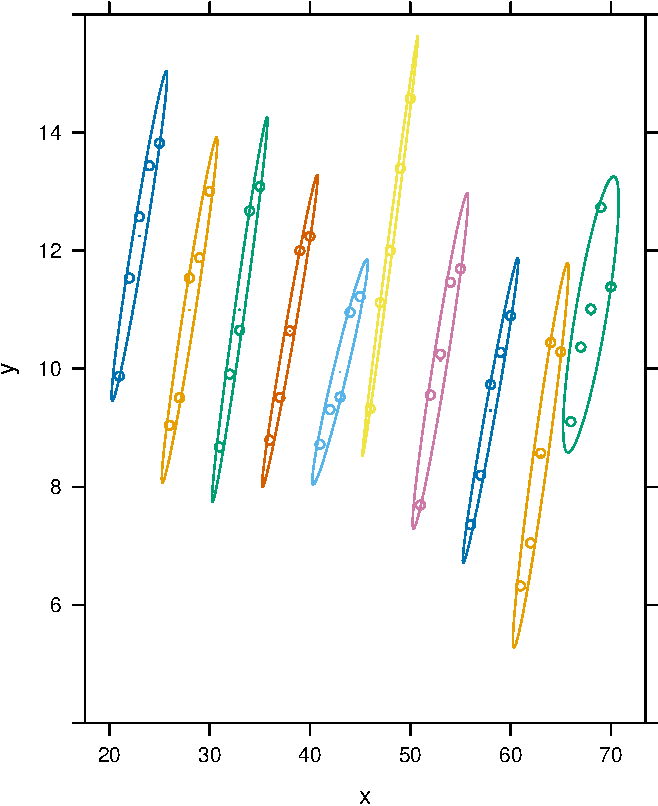
\includegraphics[width=1\linewidth]{JSS-article_files/figure-latex/plot1-1} 

}

\caption[Hierarchical data set, showing the first 10 of 100 students]{Hierarchical data set, showing the first 10 of 100 students.}\label{fig:plot1}
\end{figure}
\end{CodeChunk}

The between-student effect of age is 0 but the within-student effect is
1. Due to the large variation in ages between students, the
least-squares regression of yodeling skill on age (for the 500
observations among all 100 students) produces an estimated slope close
to 0 (though with a small \(p\)-value), because the slope is heavily
weighted toward the between-student effect:

\begin{CodeChunk}
\begin{CodeInput}
R> summary(lm(y ~ x, data=Data))
\end{CodeInput}
\begin{CodeOutput}

Call:
lm(formula = y ~ x, data = Data)

Residuals:
    Min      1Q  Median      3Q     Max 
-5.7713 -1.6583 -0.0894  1.5520  7.6240 

Coefficients:
            Estimate Std. Error t value Pr(>|t|)
(Intercept) 9.050430   0.347189  26.068  < 2e-16
x           0.020908   0.007273   2.875  0.00422

Residual standard error: 2.347 on 498 degrees of freedom
Multiple R-squared:  0.01632,   Adjusted R-squared:  0.01435 
F-statistic: 8.263 on 1 and 498 DF,  p-value: 0.004219
\end{CodeOutput}
\end{CodeChunk}

The initial mixed-effects model that we fit to the data is a simple
random-intercepts model:

\begin{CodeChunk}
\begin{CodeInput}
R> # random intercept only:
R> mod.0 <- lmer(y ~ 1 + (1 | group), Data)
R> summary(mod.0)
\end{CodeInput}
\begin{CodeOutput}
Linear mixed model fit by REML ['lmerMod']
Formula: y ~ 1 + (1 | group)
   Data: Data

REML criterion at convergence: 2103.1

Scaled residuals: 
     Min       1Q   Median       3Q      Max 
-2.03514 -0.72645 -0.01169  0.78477  2.04377 

Random effects:
 Groups   Name        Variance Std.Dev.
 group    (Intercept) 2.900    1.703   
 Residual             2.712    1.647   
Number of obs: 500, groups:  group, 100

Fixed effects:
            Estimate Std. Error t value
(Intercept)  10.0018     0.1855   53.91
\end{CodeOutput}
\end{CodeChunk}

We will shortly consider three other, more complex, mixed models;
because of data-management considerations, it is convenient to fit them
now, but we defer discussion of these models:

\begin{CodeChunk}
\begin{CodeInput}
R> # effect of x and random intercept:
R> mod.1 <- lmer(y ~ x + (1 | group), Data)
R> 
R> # effect of x, contextual (student) mean of x, and random intercept:
R> mod.2 <- lmer(y ~ x + xm + (1 | group), Data)
R>         # equivalent to y ~ I(x - xm) + xm + (1 | group)
R> 
R> # model generating the data (where Bb = 0)
R> mod.3 <- lmer(y ~ I(x - xm) + (1 | group), Data)
\end{CodeInput}
\end{CodeChunk}

We proceed to obtain predictions from the random-intercept model
(\texttt{mod.0}) and the other models (\texttt{mod.1}, \texttt{mod.2},
and \texttt{mod.3}) based on fixed effects alone, as would be used for
cross-validation based on clusters (i.e., students), and for fixed and
random effects---so-called best linear unbiased predictions or
BLUPs---as would be used for cross-validation based on cases (i.e.,
occasions within students):

\begin{CodeChunk}
\begin{CodeInput}
R> Data <- within(Data, {
+   fit_mod0.fe <- predict(mod.0, re.form = ~ 0) # fixed effects only
+   fit_mod0.re <- predict(mod.0) # fixed and random effects (BLUPs)
+   fit_mod1.fe <- predict(mod.1, re.form = ~ 0)
+   fit_mod1.re <- predict(mod.1)
+   fit_mod2.fe <- predict(mod.2, re.form = ~ 0)
+   fit_mod2.re <- predict(mod.2)
+   fit_mod3.fe <- predict(mod.3, re.form = ~ 0)
+   fit_mod3.re <- predict(mod.3)
+ })
\end{CodeInput}
\end{CodeChunk}

We then prepare the data for plotting:

\begin{CodeChunk}
\begin{CodeInput}
R> Data_long <- reshape(Data[1:Nx, ], direction = "long", sep = ".", 
+               timevar = "effect", varying = grep("\\.", names(Data[1:Nx, ])))
R> Data_long$id <- 1:nrow(Data_long)
R> Data_long <- reshape(Data_long, direction = "long", sep = "_", 
+               timevar = "modelcode",  varying = grep("_", names(Data_long)))
R> Data_long$model <- factor(
+   c("~ 1", "~ 1 + x", "~ 1 + x + xm", "~ 1 + I(x - xm)")
+   [match(Data_long$modelcode, c("mod0", "mod1", "mod2", "mod3"))]
+ )
\end{CodeInput}
\end{CodeChunk}

Predictions based on the random-intercept model \texttt{mod.0} for the
first 10 students are shown in the following graph:

\begin{CodeChunk}
\begin{CodeInput}
R> (plot +
+   xyplot(fit ~ x, subset(Data_long, modelcode == "mod0" & effect == "fe"),
+          groups=group, type="l", lwd=2) +
+   xyplot(fit ~ x, subset(Data_long, modelcode == "mod0" &  effect == "re"),
+          groups=group, type="l", lwd=2, lty=3)
+ ) |> update(
+   main="Model: y ~ 1 + (1 | group)",
+   key=list(
+     corner=c(0.05, 0.05),
+     text=list(c("fixed effects only","fixed and random")),
+     lines=list(lty=c(1, 3))))
\end{CodeInput}
\begin{figure}

{\centering 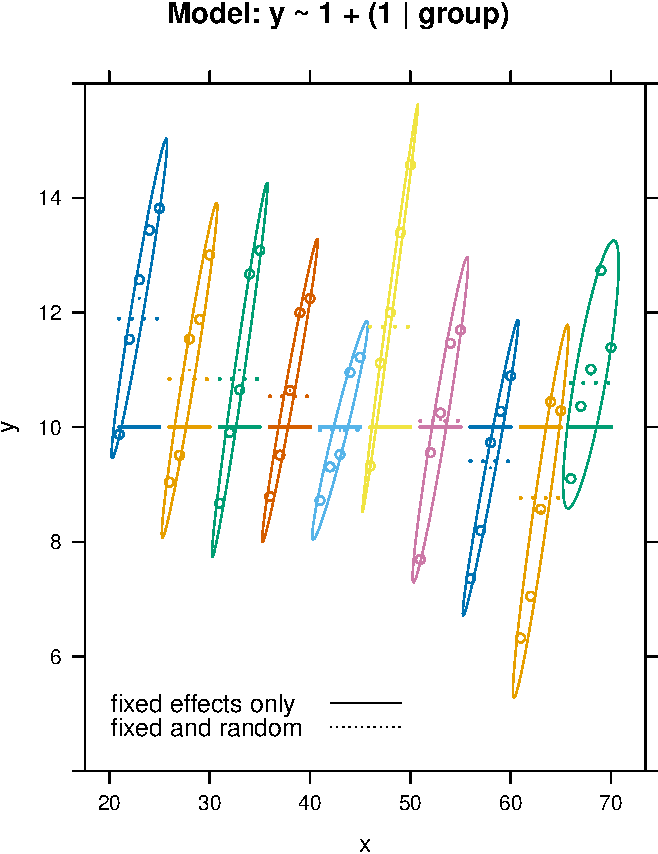
\includegraphics[width=1\linewidth]{JSS-article_files/figure-latex/plot-fits-mod0-1} 

}

\caption[Predictions from the random intercept model]{Predictions from the random intercept model.}\label{fig:plot-fits-mod0}
\end{figure}
\end{CodeChunk}

The fixed-effect predictions for the various individuals are
identical---the estimated fixed-effects intercept or estimated general
mean of \(y\)---while the BLUPs are the sums of the fixed-effects
intercept and the random intercepts, and are only slightly shrunken
towards the general mean. Because in our artificial data there is no
population relationship between age and skill, the fixed-effect-only
predictions and the BLUPs are not very different.

Our next model, \texttt{mod.1}, includes a fixed intercept and fixed
effect of \texttt{x} along with a random intercept:

\begin{CodeChunk}
\begin{CodeInput}
R> summary(mod.1)
\end{CodeInput}
\begin{CodeOutput}
Linear mixed model fit by REML ['lmerMod']
Formula: y ~ x + (1 | group)
   Data: Data

REML criterion at convergence: 1564.5

Scaled residuals: 
     Min       1Q   Median       3Q      Max 
-2.90160 -0.63501  0.01879  0.55407  2.82932 

Random effects:
 Groups   Name        Variance Std.Dev.
 group    (Intercept) 192.9406 13.8903 
 Residual               0.2569  0.5068 
Number of obs: 500, groups:  group, 100

Fixed effects:
             Estimate Std. Error t value
(Intercept) -33.91892    1.56446  -21.68
x             0.96529    0.01581   61.05

Correlation of Fixed Effects:
  (Intr)
x -0.460
\end{CodeOutput}
\end{CodeChunk}

Predictions from this model appear in the following graph:

\begin{CodeChunk}
\begin{CodeInput}
R> (plot +
+   xyplot(fit ~ x, subset(Data_long, modelcode == "mod1" & effect == "fe"),
+          groups=group, type="l", lwd=2) +
+   xyplot(fit ~ x, subset(Data_long, modelcode == "mod1" & effect == "re"),
+          groups=group, type="l", lwd=2, lty=3)
+ ) |> update(
+   main="Model: y ~ 1 + x + (1 | group)",
+   ylim=c(-15, 35),
+   key=list(
+     corner=c(0.95, 0.05),
+     text=list(c("fixed effects only","fixed and random")),
+     lines=list(lty=c(1, 3))))
\end{CodeInput}
\begin{figure}

{\centering 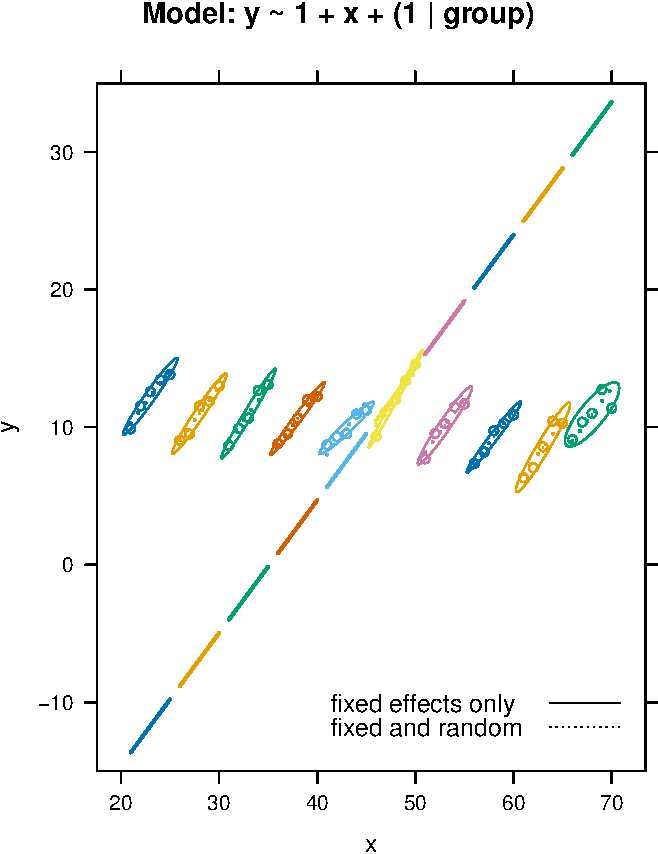
\includegraphics[width=1\linewidth]{JSS-article_files/figure-latex/plot-fits-mod1-1} 

}

\caption[Predictions from the model with random intercepts and $x$ as a fixed-effect predictor]{Predictions from the model with random intercepts and $x$ as a fixed-effect predictor.}\label{fig:plot-fits-mod1}
\end{figure}
\end{CodeChunk}

The BLUPs fit the observed data very closely, but predictions based on
the fixed effects alone, with a common intercept and slope for all
clusters, are very poor---indeed, much worse than the fixed-effects-only
predictions based on the simpler random-intercept model, \texttt{mod.0}.
We therefore anticipate (and show later in this section) that case-based
cross-validation will prefer \texttt{mod1} to \texttt{mod0}, but that
cluster-based cross-validation will prefer \texttt{mod0} to
\texttt{mod1}.

Our third model, \texttt{mod.2}, includes the contextual effect of
\(x\)---that is, the cluster mean \texttt{xm}---along with \(x\) and the
intercept in the fixed-effect part of the model, and a random intercept:

\begin{CodeChunk}
\begin{CodeInput}
R> summary(mod.2)
\end{CodeInput}
\begin{CodeOutput}
Linear mixed model fit by REML ['lmerMod']
Formula: y ~ x + xm + (1 | group)
   Data: Data

REML criterion at convergence: 1169.2

Scaled residuals: 
     Min       1Q   Median       3Q      Max 
-2.98466 -0.63750  0.00191  0.55682  2.73246 

Random effects:
 Groups   Name        Variance Std.Dev.
 group    (Intercept) 3.3986   1.8435  
 Residual             0.2552   0.5052  
Number of obs: 500, groups:  group, 100

Fixed effects:
            Estimate Std. Error t value
(Intercept)  9.47866    0.61705   15.36
x            0.99147    0.01597   62.07
xm          -0.97998    0.02055  -47.68

Correlation of Fixed Effects:
   (Intr) x     
x   0.000       
xm -0.600 -0.777
\end{CodeOutput}
\end{CodeChunk}

This model is equivalent to fitting
\texttt{y\ \textasciitilde{}\ I(x\ -\ xm)\ +\ xm\ +\ (1\ \textbar{}\ group)},
which is the model that generated the data once the coefficient of the
contextual predictor \texttt{xm} is set to 0 (as it is in
\texttt{mod.3}, discussed below).

Predictions from model \texttt{mod.2} appear in the following graph:

\begin{CodeChunk}
\begin{CodeInput}
R> (plot +
+   xyplot(fit ~ x, subset(Data_long, modelcode == "mod2" & effect == "fe"),
+          groups=group, type="l", lwd=2) +
+   xyplot(fit ~ x, subset(Data_long, modelcode == "mod2" & effect == "re"),
+          groups=group, type="l", lwd=2, lty=3)
+ ) |> update(
+   main="Model: y ~ 1 + x + xm + (1 | group)",
+   ylim=c(4, 16),
+   key=list(
+     corner=c(0.05, 0.05),
+     text=list(c("fixed effects only","fixed and random")),
+     lines=list(lty=c(1, 3))))
\end{CodeInput}
\begin{figure}

{\centering 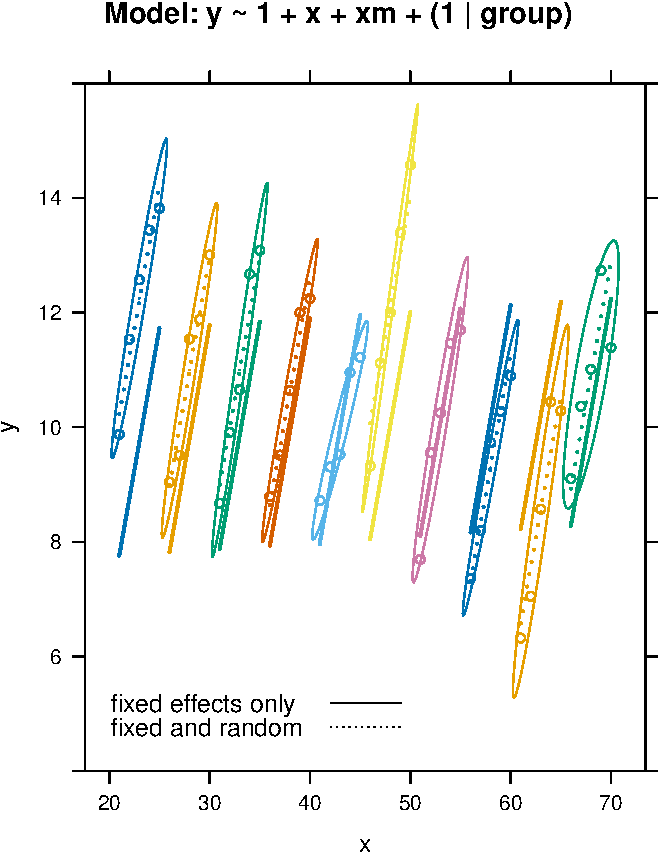
\includegraphics[width=1\linewidth]{JSS-article_files/figure-latex/plot-fits-mod2-1} 

}

\caption[Predictors from the model with random intercepts, $x$, and the group (student) mean of $x$ as predictors]{Predictors from the model with random intercepts, $x$, and the group (student) mean of $x$ as predictors.}\label{fig:plot-fits-mod2}
\end{figure}
\end{CodeChunk}

Depending on the estimated variance parameters of the model, a mixed
model like \texttt{mod.2} will apply varying degrees of shrinkage to the
random-intercept BLUPs that correspond to variation in the heights of
the parallel fitted lines for the individual students. In our contrived
data, the \texttt{mod.2} applies little shrinkage, allowing substantial
variability in the heights of the fitted lines, which closely approach
the observed values for each student. The fit of the mixed model
\texttt{mod.2} is consequently similar to that of a fixed-effects model
with age and a categorical predictor for individual students (i.e.,
treating students as a factor, and not shown here).

The mixed model \texttt{mod.2} therefore fits individual observations
well, and we anticipate a favorable assessment using individual-based
cross-validation. In contrast, the large variability in the BLUPs
results in larger residuals for predictions based on fixed effects
alone, and so we expect that cluster-based cross-validation won't show
an advantage for model \texttt{mod.2} compared to the smaller model
\texttt{mod.0}, which includes only fixed and random intercepts.

Had the mixed model applied considerable shrinkage, then neither
cluster-based nor case-based cross-validation would show much
improvement over the random-intercept-only model. In our experience, the
degree of shrinkage does not vary smoothly as parameters are changed but
tends to be ``all or nothing,'' and near the tipping point, the behavior
of estimates can be affected considerably by the choice of algorithm
used to fit the model.

Finally, \texttt{mod.3} directly estimates the model used to generate
the data. As mentioned, it is a constrained version of \texttt{mod.2},
with the coefficient of \texttt{xm} set to 0, and with \texttt{x}
expressed as a deviation from the cluster mean \texttt{xm}:

\begin{CodeChunk}
\begin{CodeInput}
R> summary(mod.3)
\end{CodeInput}
\begin{CodeOutput}
Linear mixed model fit by REML ['lmerMod']
Formula: y ~ I(x - xm) + (1 | group)
   Data: Data

REML criterion at convergence: 1163.2

Scaled residuals: 
     Min       1Q   Median       3Q      Max 
-2.97703 -0.63204  0.00627  0.56032  2.72489 

Random effects:
 Groups   Name        Variance Std.Dev.
 group    (Intercept) 3.3913   1.8415  
 Residual             0.2552   0.5052  
Number of obs: 500, groups:  group, 100

Fixed effects:
            Estimate Std. Error t value
(Intercept) 10.00176    0.18553   53.91
I(x - xm)    0.99147    0.01597   62.07

Correlation of Fixed Effects:
          (Intr)
I(x - xm) 0.000 
\end{CodeOutput}
\end{CodeChunk}

The predictions from \texttt{mod.3} are therefore similar to those from
\texttt{mod.2}:

\begin{CodeChunk}
\begin{CodeInput}
R> (plot +
+   xyplot(fit ~ x, subset(Data_long, modelcode == "mod3" & effect == "fe"),
+          groups=group, type="l", lwd=2) +
+   xyplot(fit ~ x, subset(Data_long, modelcode == "mod3" & effect == "re"),
+          groups=group, type="l", lwd=2, lty=3)
+ ) |> update(
+   main="Model: y ~ 1 + I(x - xm) + (1 | group)",
+   ylim=c(4, 16),
+   key=list(
+     corner=c(0.05, 0.05),
+     text=list(c("fixed effects only","fixed and random")),
+     lines=list(lty=c(1, 3))))
\end{CodeInput}
\begin{figure}

{\centering 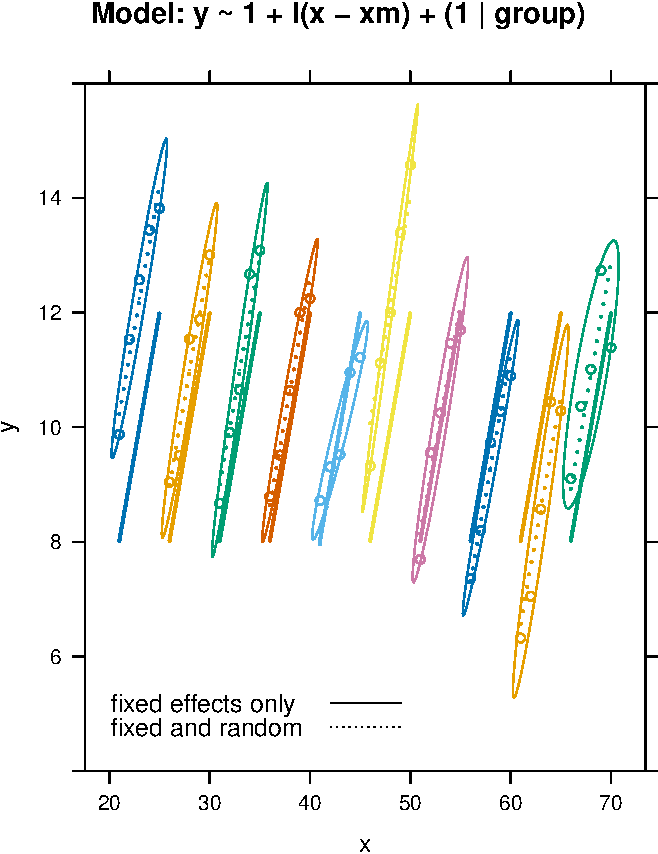
\includegraphics[width=1\linewidth]{JSS-article_files/figure-latex/plot-fits-mod3-1} 

}

\caption[Predictions from the estimated model generating the data]{Predictions from the estimated model generating the data.}\label{fig:plot-fits-mod3}
\end{figure}
\end{CodeChunk}

We next carry out case-based cross-validation, which, as we have
explained, is based on both fixed and predicted random effects (i.e.,
BLUPs), and cluster-based cross-validation, which is based on fixed
effects only. In order to reduce between-model random variability in
comparisons of models, we apply \texttt{cv()} to the list of models
created by the \texttt{models()} function (introduced previously),
performing cross-validation with the same folds for each model:

\begin{CodeChunk}
\begin{CodeInput}
R> modlist <- models("~ 1"=mod.0, "~ 1 + x"=mod.1, 
+                   "~ 1 + x + xm"=mod.2, "~ 1 + I(x - xm)"=mod.3)
R> cvs_clusters <- cv(modlist, data=Data, cluster="group", k=10, seed=6449)
R> plot(cvs_clusters, main="Model Comparison, Cluster-Based CV")
\end{CodeInput}
\begin{figure}

{\centering 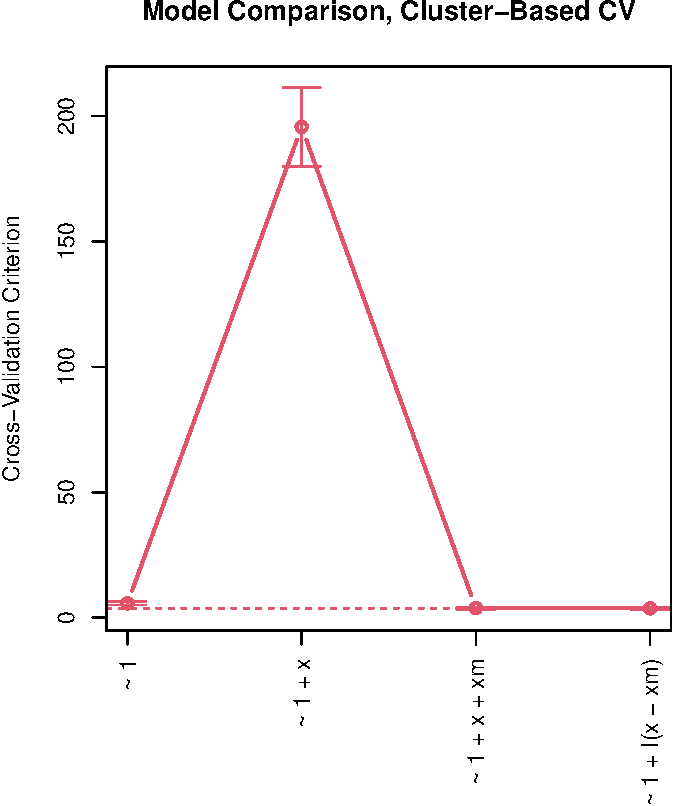
\includegraphics[width=1\linewidth]{JSS-article_files/figure-latex/cross-validation-clusters-1} 

}

\caption[10-fold cluster-based cross-validation comparing random intercept models with varying fixed effects]{10-fold cluster-based cross-validation comparing random intercept models with varying fixed effects. The error bars show the 95\% confidence interval around the CV estimate of the MSE for each model.}\label{fig:cross-validation-clusters}
\end{figure}
\end{CodeChunk}

\begin{CodeChunk}
\begin{CodeInput}
R> cvs_cases <- cv(modlist, data=Data, seed=9693)
R> plot(cvs_cases, main="Model Comparison, Case-Based CV")
\end{CodeInput}
\begin{figure}

{\centering 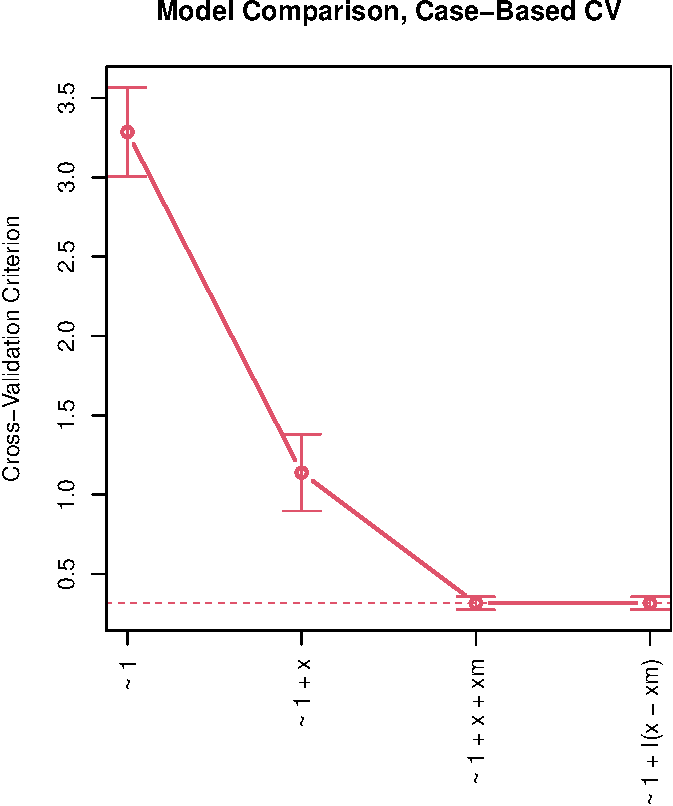
\includegraphics[width=1\linewidth]{JSS-article_files/figure-latex/cross-validation-cases-1} 

}

\caption[10-fold case-based cross-validation comparing random intercept models with varying fixed effects]{10-fold case-based cross-validation comparing random intercept models with varying fixed effects.}\label{fig:cross-validation-cases}
\end{figure}
\end{CodeChunk}

In summary, model \texttt{mod.1}, with \(x\) alone and without the
contextual mean of \(x\), is assessed as fitting very poorly by
cluster-based CV, but relatively much better by case-based CV. Model
\texttt{mod.2}, which includes both \(x\) and its contextual mean,
produces better results using both cluster-based and case-based CV. The
data-generating model, \texttt{mod.3}, which includes the fixed effect
of \texttt{x\ -\ xm} in place of separate terms in \texttt{x} and
\texttt{xm}, isn't distinguishable from model \texttt{mod.2}, which
includes \texttt{x} and \texttt{xm} separately, even though
\texttt{mod.2} has an unnecessary parameter (recall that the population
coefficient of \texttt{xm} is 0 when \texttt{x} is expressed as
deviations from the contextual mean). These conclusions are consistent
with our observations based on graphing predictions from the various
models, and they illustrate the desirability of assessing mixed-effect
models at different hierarchical levels.

\hypertarget{example-crossed-random-effects}{%
\subsection{Example: Crossed random
effects}\label{example-crossed-random-effects}}

Crossed random effects arise when the structure of the data aren't
strictly hierarchical. Nevertheless, crossed and nested random effects
can be handled in much the same manner, by refitting the mixed-effects
model to the data with a fold of clusters or cases removed and using the
refitted model to predict the response in the removed fold.

We'll illustrate with data on pig growth, introduced by \citet[Table
3.1]{DiggleLiangZeger:1994}. The data are in the \texttt{Pigs} data
frame in the \textbf{cv} package:

\begin{CodeChunk}
\begin{CodeInput}
R> head(Pigs, 9)
\end{CodeInput}
\begin{CodeOutput}
  id week weight
1  1    1   24.0
2  1    2   32.0
3  1    3   39.0
4  1    4   42.5
5  1    5   48.0
6  1    6   54.5
7  1    7   61.0
8  1    8   65.0
9  1    9   72.0
\end{CodeOutput}
\begin{CodeInput}
R> head(xtabs(~ id + week, data=Pigs), 3)
\end{CodeInput}
\begin{CodeOutput}
   week
id  1 2 3 4 5 6 7 8 9
  1 1 1 1 1 1 1 1 1 1
  2 1 1 1 1 1 1 1 1 1
  3 1 1 1 1 1 1 1 1 1
\end{CodeOutput}
\begin{CodeInput}
R> tail(xtabs(~ id + week, data=Pigs), 3)
\end{CodeInput}
\begin{CodeOutput}
    week
id   1 2 3 4 5 6 7 8 9
  46 1 1 1 1 1 1 1 1 1
  47 1 1 1 1 1 1 1 1 1
  48 1 1 1 1 1 1 1 1 1
\end{CodeOutput}
\end{CodeChunk}

Each of 48 pigs is observed weekly over a period of 9 weeks, with the
weight of the pig recorded in kg. The data are in ``long'' format, as is
appropriate for use with the \texttt{lmer()} function in the
\textbf{lme4} package. The data are very regular, with no missing cases.

The following graph, showing the growth trajectories of the pigs, is
similar to Figure 3.1 in \citet{DiggleLiangZeger:1994}; we add an
overall least-squares line and a loess smooth, which are nearly
indistinguishable:

\begin{CodeChunk}
\begin{CodeInput}
R> plot(weight ~ week, data=Pigs, type="n")
R> for (i in unique(Pigs$id)){
+   with(Pigs, lines(x=1:9, y=Pigs[id == i, "weight"],
+                    col="gray"))
+ }
R> abline(lm(weight ~ week, data=Pigs), col="blue", lwd=2)
R> lines(with(Pigs, loess.smooth(week, weight, span=0.5)),
+       col="magenta", lty=2, lwd=2)
\end{CodeInput}
\begin{figure}

{\centering 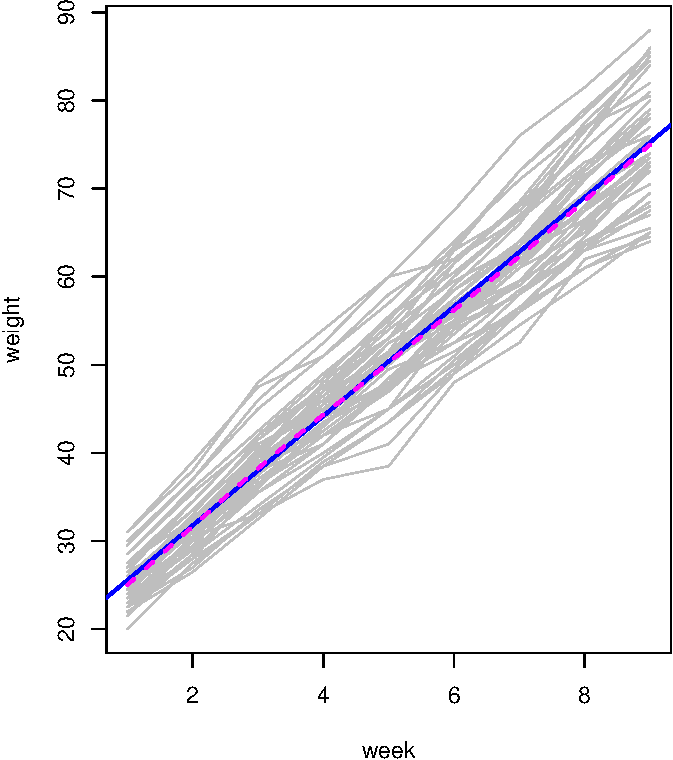
\includegraphics[width=0.6\linewidth]{JSS-article_files/figure-latex/pigs-graph-1} 

}

\caption[Growth trajectories for 48 pigs, with overall least-squares line (sold blue) and loess line (broken magenta)]{Growth trajectories for 48 pigs, with overall least-squares line (sold blue) and loess line (broken magenta).}\label{fig:pigs-graph}
\end{figure}
\end{CodeChunk}

The individual ``growth curves'' and the overall trend are generally
linear, with some tendency for variability of pig weight to increase
over weeks (a feature of the data that we ignore in the mixed model that
we fit to the data below).

The \textbf{Stata} mixed-effects models manual proposes a model with
crossed random effects for the \texttt{Pigs} data \citep[ page
37]{Stata:2023}:

\begin{quote}
{[}S{]}uppose that we wish to fit \[
\mathrm{weight}_{ij} = \beta_0 + \beta_1 \mathrm{week}_{ij} + u_i + v_j + \varepsilon_{ij} 
\] for the \(i = 1, \ldots, 9\) weeks and \(j = 1, \dots, 48\) pigs and
\[
u_i \sim N(0, \sigma^2_u); v_j \sim N(0, \sigma^2_v ); \varepsilon_{ij} \sim N(0, \sigma^2_\varepsilon)
\] all independently. That is, we assume an overall population-average
growth curve \(\beta_0 + \beta_1 \mathrm{week}\) and a random
pig-specific shift. In other words, the effect due to week, \(u_i\), is
systematic to that week and common to all pigs. The rationale behind
{[}this model{]} could be that, assuming that the pigs were measured
contemporaneously, we might be concerned that week-specific random
factors such as weather and feeding patterns had significant systematic
effects on all pigs.
\end{quote}

Although we might prefer an alternative model,\footnote{These are
  repeated-measures data, which would be more conventionally modeled
  with autocorrelated errors within pigs. The \texttt{lme()} function in
  the \textbf{nlme} package, for example, is capable of fitting a
  mixed-model of this form.} we think that this is a reasonable
specification.

The \textbf{Stata} manual fits the mixed model by maximum likelihood
(rather than REML), and we duplicate the results reported there using
\texttt{lmer()}:

\begin{CodeChunk}
\begin{CodeInput}
R> m.p <- lmer(weight ~ week + (1 | id) + (1 | week),
+             data=Pigs, REML=FALSE, # i.e., ML
+             control=lmerControl(optimizer="bobyqa"))
R> summary(m.p)
\end{CodeInput}
\begin{CodeOutput}
Linear mixed model fit by maximum likelihood  ['lmerMod']
Formula: weight ~ week + (1 | id) + (1 | week)
   Data: Pigs
Control: lmerControl(optimizer = "bobyqa")

     AIC      BIC   logLik deviance df.resid 
  2037.6   2058.0  -1013.8   2027.6      427 

Scaled residuals: 
    Min      1Q  Median      3Q     Max 
-3.7750 -0.5418  0.0054  0.4762  3.9816 

Random effects:
 Groups   Name        Variance Std.Dev.
 id       (Intercept) 14.83622 3.8518  
 week     (Intercept)  0.08499 0.2915  
 Residual              4.29733 2.0730  
Number of obs: 432, groups:  id, 48; week, 9

Fixed effects:
            Estimate Std. Error t value
(Intercept) 19.35561    0.63340   30.56
week         6.20990    0.05393  115.14

Correlation of Fixed Effects:
     (Intr)
week -0.426
\end{CodeOutput}
\end{CodeChunk}

We opt for the non-default \texttt{"bobyqa"} optimizer because it
provides more numerically stable results for subsequent cross-validation
in this example.

We can then cross-validate the model by omitting folds composed of pigs,
folds composed of weeks, or folds composed of pig-weeks (which in the
\texttt{Pigs} data set correspond to individual cases, using only the
fixed effects):

\begin{CodeChunk}
\begin{CodeInput}
R> cv(m.p, clusterVariables="id")
\end{CodeInput}
\begin{CodeOutput}
n-Fold Cross Validation based on 48 {id} clusters
cross-validation criterion = 19.97309
bias-adjusted cross-validation criterion = 19.96496
95% CI for bias-adjusted CV criterion = (17.1249, 22.80502)
full-sample criterion = 19.20076 
\end{CodeOutput}
\begin{CodeInput}
R> cv(m.p, clusterVariables="week")
\end{CodeInput}
\begin{CodeOutput}
boundary (singular) fit: see help('isSingular')
\end{CodeOutput}
\begin{CodeOutput}
n-Fold Cross Validation based on 9 {week} clusters
cross-validation criterion = 19.31219
bias-adjusted cross-validation criterion = 19.30499
95% CI for bias-adjusted CV criterion = (16.56624, 22.04373)
full-sample criterion = 19.20076 
\end{CodeOutput}
\begin{CodeInput}
R> cv(m.p, clusterVariables=c("id", "week"), k=10, seed=8469)
\end{CodeInput}
\begin{CodeOutput}
R RNG seed set to 8469
\end{CodeOutput}
\begin{CodeOutput}
10-Fold Cross Validation based on 432 {id, week} clusters
cross-validation criterion = 19.2352
bias-adjusted cross-validation criterion = 19.23294
95% CI for bias-adjusted CV criterion = (16.49263, 21.97325)
full-sample criterion = 19.20076 
\end{CodeOutput}
\end{CodeChunk}

We can also cross-validate the individual cases taking account of the
random effects (employing the same 10 folds):

\begin{CodeChunk}
\begin{CodeInput}
R> cv(m.p, k=10, seed=8469)
\end{CodeInput}
\begin{CodeOutput}
R RNG seed set to 8469
\end{CodeOutput}
\begin{CodeOutput}
10-Fold Cross Validation
cross-validation criterion = 5.15835
bias-adjusted cross-validation criterion = 5.072933
95% CI for bias-adjusted CV criterion = (4.122952, 6.022913)
full-sample criterion = 3.795972 
\end{CodeOutput}
\end{CodeChunk}

Because these predictions are based on BLUPs, they are more accurate
than the predictions based only on fixed effects.\footnote{Even though
  there is only one observation per combination of pigs and weeks, we
  can use the BLUP for the omitted case because of the crossed structure
  of the random effects; that is each pig-week has a pig random effect
  and a week random effect. Although it probably isn't sensible, we can
  imagine a mixed model for the pig data that employs nested random
  effects, which would be specified by
  \texttt{lmer(weight\ \textasciitilde{}\ week\ +\ (1\ \textbar{}\ id/week),\ data=Pigs)}---that
  is, a random intercept that varies by combinations of \texttt{id}
  (pig) and \texttt{week}. This model can't be fit, however: With only
  one case per combination of \texttt{id} and \texttt{week}, the nested
  random-effect variance is indistinguishable from the case-level
  variance.} As well, the difference between the MSE computed for the
model fit to the full data and the CV estimates of the MSE is greater
here than for cluster-based predictions.

\hypertarget{replicating-cross-validation}{%
\section{Replicating
cross-validation}\label{replicating-cross-validation}}

Assuming that the number of cases \(n\) is a multiple of the number of
folds \(k\)---a slightly simplifying assumption---the number of possible
partitions of cases into folds is \(\frac{n!}{[(n/k)!]^k}\), a number
that grows very large very quickly. For example, for \(n = 10\) and
\(k = 5\), so that the folds are each of size \(n/k = 2\), there are
\(113,400\) possible partitions; for \(n=100\) and \(k=5\), where
\(n/k = 20\), still a small problem, the number of possible partitions
is truly astronomical, \(1.09\times 10^{66}\).

Because the partition into folds that's employed is selected randomly,
the resulting CV criterion estimates are subject to sampling error. (An
exception is LOO cross-validation, which is not at all random.) To get a
sense of the magnitude of the sampling error, we can repeat the CV
procedure with different randomly selected partitions into folds. All of
the CV functions in the \textbf{cv} package are capable of repeated
cross-validation, with the number of repetitions controlled by the
\texttt{reps} argument, which defaults to \texttt{1}.

Here, for example, is 10-fold CV for the Mroz logistic regression,
repeated 5 times:

\begin{CodeChunk}
\begin{CodeInput}
R> cv(m.mroz, criterion=BayesRule, seed=248, reps=5, 
+    method="Woodbury")
\end{CodeInput}
\begin{CodeOutput}
R RNG seed set to 248
\end{CodeOutput}
\begin{CodeOutput}
R RNG seed set to 68134
\end{CodeOutput}
\begin{CodeOutput}
R RNG seed set to 767359
\end{CodeOutput}
\begin{CodeOutput}
R RNG seed set to 556270
\end{CodeOutput}
\begin{CodeOutput}
R RNG seed set to 882966
\end{CodeOutput}
\begin{CodeOutput}

Replicate 1:
10-Fold Cross Validation
method: Woodbury
criterion: BayesRule
cross-validation criterion = 0.3200531
bias-adjusted cross-validation criterion = 0.3130109
95% CI for bias-adjusted CV criterion = (0.2796692, 0.3463526)
full-sample criterion = 0.3067729 

Replicate 2:
10-Fold Cross Validation
method: Woodbury
criterion: BayesRule
cross-validation criterion = 0.3160691
bias-adjusted cross-validation criterion = 0.311697
95% CI for bias-adjusted CV criterion = (0.2784665, 0.3449274)
full-sample criterion = 0.3067729 

Replicate 3:
10-Fold Cross Validation
method: Woodbury
criterion: BayesRule
cross-validation criterion = 0.314741
bias-adjusted cross-validation criterion = 0.3086212
95% CI for bias-adjusted CV criterion = (0.2754285, 0.341814)
full-sample criterion = 0.3067729 

Replicate 4:
10-Fold Cross Validation
method: Woodbury
criterion: BayesRule
cross-validation criterion = 0.3240372
bias-adjusted cross-validation criterion = 0.318069
95% CI for bias-adjusted CV criterion = (0.2846189, 0.3515192)
full-sample criterion = 0.3067729 

Replicate 5:
10-Fold Cross Validation
method: Woodbury
criterion: BayesRule
cross-validation criterion = 0.3240372
bias-adjusted cross-validation criterion = 0.3192577
95% CI for bias-adjusted CV criterion = (0.2858076, 0.3527079)
full-sample criterion = 0.3067729 

Average:
10-Fold Cross Validation
method: Woodbury
criterion: BayesRule
cross-validation criterion = 0.3198318 (0.003886968)
bias-adjusted cross-validation criterion = 0.3139445 (0.004009339)
full-sample criterion = 0.3067729 
\end{CodeOutput}
\end{CodeChunk}

When \texttt{reps} \textgreater{} \texttt{1}, the result returned by
\texttt{cv()} is an object of class \texttt{"cvList"}---literally a list
of \texttt{"cv"} objects. The results are reported for each repetition
and then averaged across repetitions, with the standard deviations of
the CV criterion and the biased-adjusted CV criterion given in
parentheses. In this example, there is therefore little variation across
repetitions, increasing our confidence in the reliability of the
results.

Notice that the seed that's set in the \texttt{cv()} command pertains to
the first repetition and the seeds for the remaining repetitions are
then selected pseudo-randomly.\footnote{Because of the manner in which
  the computation is performed, the order of the replicates in the
  \texttt{"cvList"} object returned by \texttt{cv()} isn't the same as
  the order in which the replicates are computed. Each element of the
  result, however, is a \texttt{"cv"} object with the correct
  random-number seed saved, and so this technical detail can be safely
  ignored. The individual \texttt{"cv"} objects are printed in the order
  in which they are stored rather than the order in which they are
  computed.} Setting the first seed, however, makes the entire process
easily replicable, and the seed for each repetition is stored in the
corresponding element of the \texttt{"cvList"} object (which isn't,
however, saved in the example).

It's also possible to replicate CV when comparing competing models via
the \texttt{cv()} method for \texttt{"modList"} objects. Recall our
comparison of polynomial regressions of varying degree fit to the
\texttt{Auto} data; we performed 10-fold CV for each of 10 models. Here,
we replicate that process 5 times for each model and graph the results:

\begin{CodeChunk}
\begin{CodeInput}
R> cv.auto.reps <- cv(models(m.1, m.2, m.3, m.4, m.5,
+                         m.6, m.7, m.8, m.9, m.10),
+                  data=Auto, seed=8004, reps=5)
R> plot(cv.auto.reps)
\end{CodeInput}
\begin{figure}

{\centering 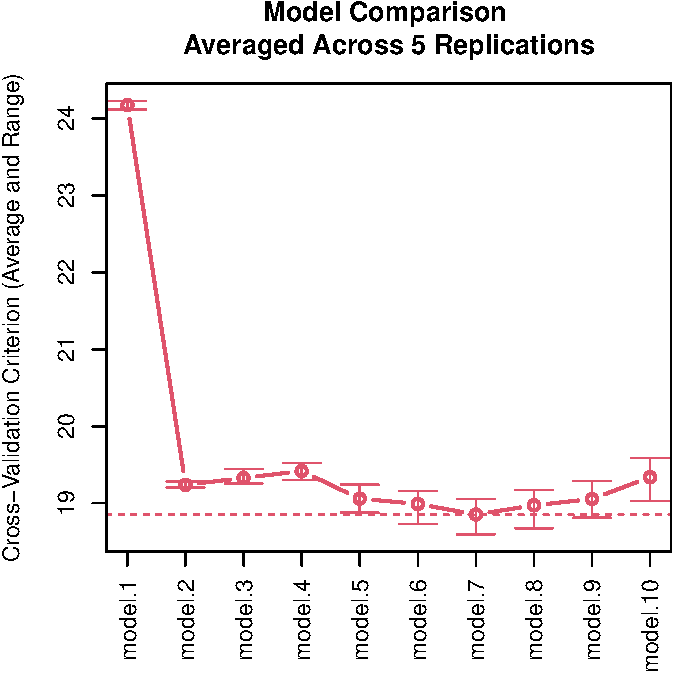
\includegraphics[width=1\linewidth]{JSS-article_files/figure-latex/model-comparison-with-reps-1} 

}

\caption[ Replicated cross-validated 10-fold CV as a function of polynomial degree, $p$]{ Replicated cross-validated 10-fold CV as a function of polynomial degree, $p$}\label{fig:model-comparison-with-reps}
\end{figure}
\end{CodeChunk}

The graph shows both the average CV criterion and its range for each of
the competing models.

\hypertarget{cross-validating-model-selection}{%
\section{Cross-validating model
selection}\label{cross-validating-model-selection}}

\hypertarget{a-preliminary-example}{%
\subsection{A preliminary example}\label{a-preliminary-example}}

As \citet[Sec. 7.10.2: ``The Wrong and Right Way to Do
Cross-validation'']{HastieTibshiraniFriedman:2009} explain, if the whole
data are used to select or fine-tune a statistical model, subsequent
cross-validation of the model is intrinsically misleading, because the
model is selected to fit the whole data, including the part of the data
that remains when each fold is removed.

The following example is similar in spirit to one employed by
\citet{HastieTibshiraniFriedman:2009}. Suppose that we randomly generate
\(n = 1000\) independent observations for a response variable variable
\(y \sim N(\mu = 10, \sigma^2 = 0)\), and independently sample \(1000\)
observations for \(p = 100\) ``predictors,'' \(x_1, \ldots, x_{100}\),
each from \(x_j \sim N(0, 1)\). The response has nothing to do with the
predictors and so the population linear-regression model
\(y_i = \alpha + \beta_1 x_{i1} + \cdots + \beta_{100} x_{i,100} + \varepsilon_i\)
has \(\alpha = 10\) and all \(\beta_j = 0\).

\begin{CodeChunk}
\begin{CodeInput}
R> set.seed(24361) # for reproducibility
R> D <- data.frame(
+   y = rnorm(1000, mean=10),
+   X = matrix(rnorm(1000*100), 1000, 100)
+ )
R> head(D[, 1:6])
\end{CodeInput}
\begin{CodeOutput}
          y        X.1        X.2         X.3         X.4         X.5
1 10.031647 -1.2388628 -0.2648705 -0.03539048 -2.57697337  0.81104761
2  9.664989  0.1228689 -0.1774440  0.37290421 -0.93513788  0.62867324
3 10.023249 -0.9505172 -0.7348667 -1.05978180  0.88294443  0.02391808
4  8.990969  1.1357103  0.3241085  0.11036901  1.37630285 -0.42211426
5  9.071249  1.4947403  1.8753802  0.10574793  0.29213991 -0.18456833
6 11.349283 -0.1845331 -0.7803709 -1.23803778 -0.01094861  0.69103395
\end{CodeOutput}
\end{CodeChunk}

Least-squares provides accurate estimates of the regression constant
\(\alpha = 10\) and the error variance \(\sigma^2 = 1\) for the ``null
model'' including only the regression constant; moreover, the omnibus
\(F\)-test of the correct null hypothesis that all of the \(\beta\)s are
0 for the ``full model'' with all 100 \(x\)s is associated with a large
\(p\)-value:

\begin{CodeChunk}
\begin{CodeInput}
R> m.full <- lm(y ~ ., data=D)
R> m.null <- lm(y ~ 1, data=D)
R> anova(m.null, m.full)
\end{CodeInput}
\begin{CodeOutput}
Analysis of Variance Table

Model 1: y ~ 1
Model 2: y ~ X.1 + X.2 + X.3 + X.4 + X.5 + X.6 + X.7 + X.8 + X.9 + X.10 + 
    X.11 + X.12 + X.13 + X.14 + X.15 + X.16 + X.17 + X.18 + X.19 + 
    X.20 + X.21 + X.22 + X.23 + X.24 + X.25 + X.26 + X.27 + X.28 + 
    X.29 + X.30 + X.31 + X.32 + X.33 + X.34 + X.35 + X.36 + X.37 + 
    X.38 + X.39 + X.40 + X.41 + X.42 + X.43 + X.44 + X.45 + X.46 + 
    X.47 + X.48 + X.49 + X.50 + X.51 + X.52 + X.53 + X.54 + X.55 + 
    X.56 + X.57 + X.58 + X.59 + X.60 + X.61 + X.62 + X.63 + X.64 + 
    X.65 + X.66 + X.67 + X.68 + X.69 + X.70 + X.71 + X.72 + X.73 + 
    X.74 + X.75 + X.76 + X.77 + X.78 + X.79 + X.80 + X.81 + X.82 + 
    X.83 + X.84 + X.85 + X.86 + X.87 + X.88 + X.89 + X.90 + X.91 + 
    X.92 + X.93 + X.94 + X.95 + X.96 + X.97 + X.98 + X.99 + X.100
  Res.Df    RSS  Df Sum of Sq      F Pr(>F)
1    999 973.65                            
2    899 888.44 100    85.208 0.8622  0.825
\end{CodeOutput}
\begin{CodeInput}
R> summary(m.null)
\end{CodeInput}
\begin{CodeOutput}

Call:
lm(formula = y ~ 1, data = D)

Residuals:
    Min      1Q  Median      3Q     Max 
-3.4585 -0.6809  0.0190  0.6365  2.9346 

Coefficients:
            Estimate Std. Error t value Pr(>|t|)
(Intercept)  9.93704    0.03122   318.3   <2e-16

Residual standard error: 0.9872 on 999 degrees of freedom
\end{CodeOutput}
\end{CodeChunk}

Next, using the \texttt{stepAIC()} function in the \textbf{MASS} package
\citep{VenablesRipley:2002}, let us perform a forward stepwise
regression to select a ``best'' model, starting with the null model, and
using AIC as the model-selection criterion (see the help page for
\texttt{stepAIC()} for details):\footnote{It's generally advantageous to
  start with the largest model, here the one with 100 predictors, and
  proceed by backward elimination. In this demonstration, however, where
  all of the \(\beta\)s are really 0, the selected model will be small,
  and so we proceed by forward selection from the null model to save
  computing time.}

\begin{CodeChunk}
\begin{CodeInput}
R> library("MASS")  # for stepAIC()
R> m.select <- stepAIC(m.null,
+                     direction="forward", trace=FALSE,
+                     scope=list(lower=~1, upper=formula(m.full)))
R> summary(m.select)
\end{CodeInput}
\begin{CodeOutput}

Call:
lm(formula = y ~ X.99 + X.90 + X.87 + X.40 + X.65 + X.91 + X.53 + 
    X.45 + X.31 + X.56 + X.61 + X.60 + X.46 + X.35 + X.92, data = D)

Residuals:
    Min      1Q  Median      3Q     Max 
-3.2620 -0.6446  0.0236  0.6406  3.1180 

Coefficients:
            Estimate Std. Error t value Pr(>|t|)
(Intercept)  9.93716    0.03098 320.803  < 2e-16
X.99        -0.09103    0.03082  -2.953  0.00322
X.90        -0.08205    0.03135  -2.617  0.00901
X.87        -0.06942    0.03105  -2.235  0.02561
X.40        -0.04759    0.03076  -1.547  0.12211
X.65        -0.05523    0.03147  -1.755  0.07952
X.91         0.05245    0.03084   1.700  0.08937
X.53        -0.04921    0.03048  -1.615  0.10672
X.45         0.05543    0.03182   1.742  0.08183
X.31         0.04525    0.03108   1.456  0.14570
X.56         0.05433    0.03273   1.660  0.09723
X.61        -0.05085    0.03170  -1.604  0.10908
X.60        -0.05133    0.03194  -1.607  0.10832
X.46         0.05158    0.03272   1.576  0.11529
X.35         0.04696    0.03146   1.493  0.13584
X.92         0.04430    0.03100   1.429  0.15329

Residual standard error: 0.9725 on 984 degrees of freedom
Multiple R-squared:  0.04419,   Adjusted R-squared:  0.02962 
F-statistic: 3.033 on 15 and 984 DF,  p-value: 8.338e-05
\end{CodeOutput}
\begin{CodeInput}
R> mse(D$y, fitted(m.select))
\end{CodeInput}
\begin{CodeOutput}
[1] 0.9306254
attr(,"casewise loss")
[1] "(y - yhat)^2"
\end{CodeOutput}
\end{CodeChunk}

The resulting model has 15 predictors, a very modest \(R^2 = .044\), but
a small \(p\)-value for its omnibus \(F\)-test (which, of course, is
entirely spurious because the same data were used to select and test the
model). The MSE for the selected model is smaller than the true error
variance \(\sigma^2 = 1\), as is the estimated error variance for the
selected model, \(\widehat{\sigma}^2 = 0.973^2 = 0.947\).

If we cross-validate the selected model, we also obtain an optimistic
estimate of its predictive power (although the confidence interval for
the bias-adjusted MSE includes 1):

\begin{CodeChunk}
\begin{CodeInput}
R> cv(m.select, seed=2529)
\end{CodeInput}
\begin{CodeOutput}
R RNG seed set to 2529
\end{CodeOutput}
\begin{CodeOutput}
10-Fold Cross Validation
method: Woodbury
criterion: mse
cross-validation criterion = 0.9593695
bias-adjusted cross-validation criterion = 0.9578478
95% CI for bias-adjusted CV criterion = (0.8766138, 1.039082)
full-sample criterion = 0.9306254 
\end{CodeOutput}
\end{CodeChunk}

The \texttt{cvSelect()} function in the \textbf{cv} package allows us to
cross-validate the whole model-selection procedure. The first argument
to \texttt{cvSelect()} is a model-selection function capable of
refitting the model with a fold omitted and returning a CV criterion.
The \texttt{selectStepAIC()} function, also in \textbf{cv} and based on
\texttt{stepAIC()}, is suitable for use with \texttt{cvSelect()}:

\begin{CodeChunk}
\begin{CodeInput}
R> cv.select <- cvSelect(selectStepAIC, data=D, seed=3791,
+                       model=m.null, direction="forward",
+                       scope=list(lower=~1, 
+                                  upper=formula(m.full)))
\end{CodeInput}
\begin{CodeOutput}
R RNG seed set to 3791
\end{CodeOutput}
\begin{CodeInput}
R> cv.select
\end{CodeInput}
\begin{CodeOutput}
10-Fold Cross Validation
cross-validation criterion = 1.06873
bias-adjusted cross-validation criterion = 1.061183
95% CI for bias-adjusted CV criterion = (0.9717229, 1.150642)
full-sample criterion = 0.9306254 
\end{CodeOutput}
\end{CodeChunk}

The other arguments to \texttt{cvSelect()} are:

\begin{itemize}
\tightlist
\item
  \texttt{data}, the data set to which the model is fit;
\item
  \texttt{seed}, an optional seed for R's pseudo-random-number
  generator; as for \texttt{cv()}, if the seed isn't supplied by the
  user, a seed is randomly selected and saved;
\item
  additional arguments required by the model-selection function, here
  the starting \texttt{model} argument, the \texttt{direction} of model
  selection, and the \texttt{scope} of models considered (from the model
  with only a regression constant to the model with all 100 predictors).
\end{itemize}

By default, \texttt{cvSelect()} performs 10-fold CV, and produces an
estimate of MSE for the model-selection procedure even \emph{larger}
than the true error variance, \(\sigma^2 = 1\).

Also by default, when the number of folds is 10 or fewer,
\texttt{cvSelect()} saves the coefficients of the selected models. In
this example, the \texttt{compareFolds()} function reveals that the
variables retained by the model-selection process in the several folds
are quite different:

\begin{CodeChunk}
\begin{CodeInput}
R> compareFolds(cv.select)
\end{CodeInput}
\begin{CodeOutput}
        (Intercept)    X.87    X.90    X.99    X.91    X.54    X.53    X.56
Fold 1       9.9187 -0.0615 -0.0994 -0.0942  0.0512  0.0516                
Fold 2       9.9451 -0.0745 -0.0899 -0.0614          0.0587          0.0673
Fold 3       9.9423 -0.0783 -0.0718 -0.0987  0.0601                  0.0512
Fold 4       9.9410 -0.0860 -0.0831 -0.0867  0.0570         -0.0508        
Fold 5       9.9421 -0.0659 -0.0849 -0.1004  0.0701  0.0511 -0.0487  0.0537
Fold 6       9.9633 -0.0733 -0.0874 -0.0960  0.0555  0.0629 -0.0478        
Fold 7       9.9279 -0.0618 -0.0960 -0.0838  0.0533         -0.0464        
Fold 8       9.9453 -0.0610 -0.0811 -0.0818          0.0497 -0.0612  0.0560
Fold 9       9.9173 -0.0663 -0.0894 -0.1100  0.0504  0.0524          0.0747
Fold 10      9.9449 -0.0745 -0.0906 -0.0891  0.0535  0.0482 -0.0583  0.0642
           X.40    X.45    X.65    X.68    X.92    X.15    X.26    X.46    X.60
Fold 1                  -0.0590                 -0.0456  0.0658  0.0608        
Fold 2                                   0.0607          0.0487                
Fold 3  -0.0496         -0.0664          0.0494                                
Fold 4  -0.0597  0.0579 -0.0531          0.0519 -0.0566                 -0.0519
Fold 5                           0.0587                          0.0527 -0.0603
Fold 6  -0.0596  0.0552          0.0474                                        
Fold 7           0.0572          0.0595                                        
Fold 8           0.0547 -0.0617  0.0453  0.0493 -0.0613  0.0591  0.0703 -0.0588
Fold 9  -0.0552  0.0573 -0.0635  0.0492         -0.0513  0.0484         -0.0507
Fold 10 -0.0558                          0.0529                  0.0710        
           X.61     X.8    X.28    X.29    X.31    X.35    X.70    X.89    X.17
Fold 1  -0.0490          0.0616 -0.0537                  0.0638                
Fold 2           0.0671                  0.0568                  0.0523        
Fold 3  -0.0631          0.0616                                                
Fold 4           0.0659         -0.0549          0.0527                  0.0527
Fold 5           0.0425                  0.0672  0.0613          0.0493        
Fold 6           0.0559         -0.0629  0.0498          0.0487                
Fold 7                                                           0.0611  0.0472
Fold 8  -0.0719                                          0.0586                
Fold 9                   0.0525                                                
Fold 10 -0.0580                                  0.0603                        
           X.25     X.4    X.64    X.81    X.97    X.11     X.2    X.33    X.47
Fold 1                                   0.0604          0.0575                
Fold 2   0.0478          0.0532  0.0518                                        
Fold 3                           0.0574                          0.0473        
Fold 4                   0.0628                                                
Fold 5   0.0518                                                                
Fold 6                                           0.0521                        
Fold 7           0.0550                                                        
Fold 8                                                                         
Fold 9                                   0.0556                          0.0447
Fold 10          0.0516                                                        
            X.6    X.72    X.73    X.77    X.79 X.88
Fold 1   0.0476                                     
Fold 2                   0.0514                     
Fold 3                                              
Fold 4                                  -0.0473     
Fold 5           0.0586                         0.07
Fold 6                          -0.0489             
Fold 7                                              
Fold 8                                              
Fold 9                                              
Fold 10                                             
\end{CodeOutput}
\end{CodeChunk}

\hypertarget{mrozs-logistic-regression-revisited}{%
\subsection{Mroz's logistic regression
revisited}\label{mrozs-logistic-regression-revisited}}

For a contrasting example we apply model selection to Mroz's logistic
regression for married women's labor-force participation. First, recall
the logistic regression model that we fit to the \texttt{Mroz} data:

\begin{CodeChunk}
\begin{CodeInput}
R> summary(m.mroz)
\end{CodeInput}
\begin{CodeOutput}

Call:
glm(formula = lfp ~ ., family = binomial, data = Mroz)

Coefficients:
             Estimate Std. Error z value Pr(>|z|)
(Intercept)  3.182140   0.644375   4.938 7.88e-07
k5          -1.462913   0.197001  -7.426 1.12e-13
k618        -0.064571   0.068001  -0.950 0.342337
age         -0.062871   0.012783  -4.918 8.73e-07
wcyes        0.807274   0.229980   3.510 0.000448
hcyes        0.111734   0.206040   0.542 0.587618
lwg          0.604693   0.150818   4.009 6.09e-05
inc         -0.034446   0.008208  -4.196 2.71e-05

(Dispersion parameter for binomial family taken to be 1)

    Null deviance: 1029.75  on 752  degrees of freedom
Residual deviance:  905.27  on 745  degrees of freedom
AIC: 921.27

Number of Fisher Scoring iterations: 4
\end{CodeOutput}
\end{CodeChunk}

Applying stepwise model selection Mroz's logistic regression, using BIC
as the model-selection criterion (via the argument
\texttt{k=log(nrow(Mroz))} to \texttt{stepAIC()}) selects 5 of the 7
original predictors:

\begin{CodeChunk}
\begin{CodeInput}
R> m.mroz.sel <- stepAIC(m.mroz, k=log(nrow(Mroz)),
+                       trace=FALSE)
R> summary(m.mroz.sel)
\end{CodeInput}
\begin{CodeOutput}

Call:
glm(formula = lfp ~ k5 + age + wc + lwg + inc, family = binomial, 
    data = Mroz)

Coefficients:
            Estimate Std. Error z value Pr(>|z|)
(Intercept)  2.90193    0.54290   5.345 9.03e-08
k5          -1.43180    0.19320  -7.411 1.25e-13
age         -0.05853    0.01142  -5.127 2.94e-07
wcyes        0.87237    0.20639   4.227 2.37e-05
lwg          0.61568    0.15014   4.101 4.12e-05
inc         -0.03367    0.00780  -4.317 1.58e-05

(Dispersion parameter for binomial family taken to be 1)

    Null deviance: 1029.75  on 752  degrees of freedom
Residual deviance:  906.46  on 747  degrees of freedom
AIC: 918.46

Number of Fisher Scoring iterations: 3
\end{CodeOutput}
\begin{CodeInput}
R> BayesRule(Mroz$lfp == "yes",
+           predict(m.mroz.sel, type="response"))
\end{CodeInput}
\begin{CodeOutput}
[1] 0.3187251
attr(,"casewise loss")
[1] "y != round(yhat)"
\end{CodeOutput}
\end{CodeChunk}

Bayes rule applied to the selected model misclassifies 32\% of the cases
in the \texttt{Mroz} data.

Cross-validating the selected model produces a similar, slightly larger,
estimate of misclassification, about 33\%:

\begin{CodeChunk}
\begin{CodeInput}
R> cv(m.mroz.sel, criterion=BayesRule, seed=345266)
\end{CodeInput}
\begin{CodeOutput}
R RNG seed set to 345266
\end{CodeOutput}
\begin{CodeOutput}
10-Fold Cross Validation
method: exact
criterion: BayesRule
cross-validation criterion = 0.3306773
bias-adjusted cross-validation criterion = 0.3333245
95% CI for bias-adjusted CV criterion = (0.2996998, 0.3669493)
full-sample criterion = 0.3187251 
\end{CodeOutput}
\end{CodeChunk}

Is this estimate of predictive performance optimistic?

We proceed to apply the model-selection procedure by cross-validation,
producing more or less the same result:

\begin{CodeChunk}
\begin{CodeInput}
R> m.mroz.sel.cv <- cvSelect(selectStepAIC, Mroz, 
+                           seed=6681,
+                           criterion=BayesRule,
+                           model=m.mroz,
+                           AIC=FALSE)
\end{CodeInput}
\begin{CodeOutput}
R RNG seed set to 6681
\end{CodeOutput}
\begin{CodeInput}
R> m.mroz.sel.cv
\end{CodeInput}
\begin{CodeOutput}
10-Fold Cross Validation
cross-validation criterion = 0.3306773
bias-adjusted cross-validation criterion = 0.3345203
95% CI for bias-adjusted CV criterion = (0.3008955, 0.368145)
full-sample criterion = 0.3187251 
\end{CodeOutput}
\end{CodeChunk}

Setting \texttt{AIC=FALSE} in the call to \texttt{cvSelect()} uses the
BIC rather than the AIC as the model-selection criterion. As it turns
out, exactly the same predictors are selected when each of the 10 folds
are omitted, and the several coefficient estimates are very similar, as
we show using \texttt{compareFolds()}:

\begin{CodeChunk}
\begin{CodeInput}
R> compareFolds(m.mroz.sel.cv)
\end{CodeInput}
\begin{CodeOutput}
        (Intercept)     age     inc      k5     lwg wcyes
Fold 1       2.5014 -0.0454 -0.0388 -1.3613  0.5653  0.85
Fold 2       3.0789 -0.0659 -0.0306 -1.5335  0.6923  0.79
Fold 3       3.0141 -0.0595 -0.0305 -1.3994  0.5428  0.86
Fold 4       2.7251 -0.0543 -0.0354 -1.4474  0.6298  1.09
Fold 5       2.7617 -0.0566 -0.0320 -1.4752  0.6324  0.74
Fold 6       3.0234 -0.0621 -0.0348 -1.4537  0.6618  0.94
Fold 7       2.9615 -0.0600 -0.0351 -1.4127  0.5835  0.97
Fold 8       2.9598 -0.0603 -0.0329 -1.3865  0.6210  0.69
Fold 9       3.2481 -0.0650 -0.0381 -1.4138  0.6093  0.94
Fold 10      2.7724 -0.0569 -0.0295 -1.4503  0.6347  0.85
\end{CodeOutput}
\end{CodeChunk}

In this example, therefore, we appear to obtain a realistic estimate of
model performance directly from the selected model, because there is
little added uncertainty induced by model selection.

\hypertarget{cross-validating-choice-of-transformations-in-regression}{%
\subsection{Cross-validating choice of transformations in
regression}\label{cross-validating-choice-of-transformations-in-regression}}

The \textbf{cv} package also provides a \texttt{cvSelect()} procedure,
\texttt{selectTrans()}, for choosing transformations of the predictors
and the response in regression.

Some background: As \citet[Sec. 8.2]{Weisberg:2014} explains, there are
technical advantages to having (numeric) predictors in linear regression
analysis that are themselves linearly related. If the predictors
\emph{aren't} linearly related, then the relationships between them can
often be straightened by power transformations. Transformations can be
selected after graphical examination of the data, or by analytic
methods. Once the relationships between the predictors are linearized,
it can be advantageous similarly to transform the response variable
towards normality.

Selecting transformations analytically raises the possibility of
automating the process, as would be required for cross-validation. One
could, in principle, apply graphical methods to select transformations
for each fold, but because a data analyst couldn't forget the choices
made for previous folds, the process wouldn't really be applied
independently to the folds.

To illustrate, we adapt an example appearing in several places in
\citet{FoxWeisberg:2019} (for example in Chapter 3 on transforming
data), using data on the prestige and other characteristics of 102
Canadian occupations circa 1970. The data are in the \texttt{Prestige}
data frame in the \textbf{carData} package:

\begin{CodeChunk}
\begin{CodeInput}
R> data("Prestige", package="carData")
R> head(Prestige)
\end{CodeInput}
\begin{CodeOutput}
                    education income women prestige census type
gov.administrators      13.11  12351 11.16     68.8   1113 prof
general.managers        12.26  25879  4.02     69.1   1130 prof
accountants             12.77   9271 15.70     63.4   1171 prof
purchasing.officers     11.42   8865  9.11     56.8   1175 prof
chemists                14.62   8403 11.68     73.5   2111 prof
physicists              15.64  11030  5.13     77.6   2113 prof
\end{CodeOutput}
\begin{CodeInput}
R> summary(Prestige)
\end{CodeInput}
\begin{CodeOutput}
   education          income          women           prestige    
 Min.   : 6.380   Min.   :  611   Min.   : 0.000   Min.   :14.80  
 1st Qu.: 8.445   1st Qu.: 4106   1st Qu.: 3.592   1st Qu.:35.23  
 Median :10.540   Median : 5930   Median :13.600   Median :43.60  
 Mean   :10.738   Mean   : 6798   Mean   :28.979   Mean   :46.83  
 3rd Qu.:12.648   3rd Qu.: 8187   3rd Qu.:52.203   3rd Qu.:59.27  
 Max.   :15.970   Max.   :25879   Max.   :97.510   Max.   :87.20  
     census       type   
 Min.   :1113   bc  :44  
 1st Qu.:3120   prof:31  
 Median :5135   wc  :23  
 Mean   :5402   NA's: 4  
 3rd Qu.:8312            
 Max.   :9517            
\end{CodeOutput}
\end{CodeChunk}

The variables in the \texttt{Prestige} data set are:

\begin{itemize}
\tightlist
\item
  \texttt{education}: average years of education for incumbents in the
  occupation, from the 1971 Canadian Census.
\item
  \texttt{income}: average dollars of annual income for the occupation,
  from the Census.
\item
  \texttt{women}: percentage of occupational incumbents who were women,
  also from the Census.
\item
  \texttt{prestige}: the average prestige rating of the occupation on a
  0--100 ``thermometer'' scale, in a Canadian social survey conducted
  around the same time.
\item
  \texttt{type}, type of occupation, and \texttt{census}, the Census
  occupational code, which are not used in our example.
\end{itemize}

The object of a regression analysis for the \texttt{Prestige} data (and
their original purpose) is to predict occupational prestige from the
other variables in the data set.

A scatterplot matrix (using the \texttt{scatterplotMatrix()} function in
the \textbf{car} package) of the numeric variables in the data reveals
that the distributions of \texttt{income} and \texttt{women} are
positively skewed, and that some of the relationships among the three
predictors, and between the predictors and the response (i.e.,
\texttt{prestige}), are nonlinear:

\begin{CodeChunk}
\begin{CodeInput}
R> library("car")
\end{CodeInput}
\begin{CodeOutput}
Loading required package: carData
\end{CodeOutput}
\begin{CodeInput}
R> scatterplotMatrix(~ prestige + income + education + women,
+                   data=Prestige, smooth=list(spread=FALSE))
\end{CodeInput}
\begin{figure}

{\centering 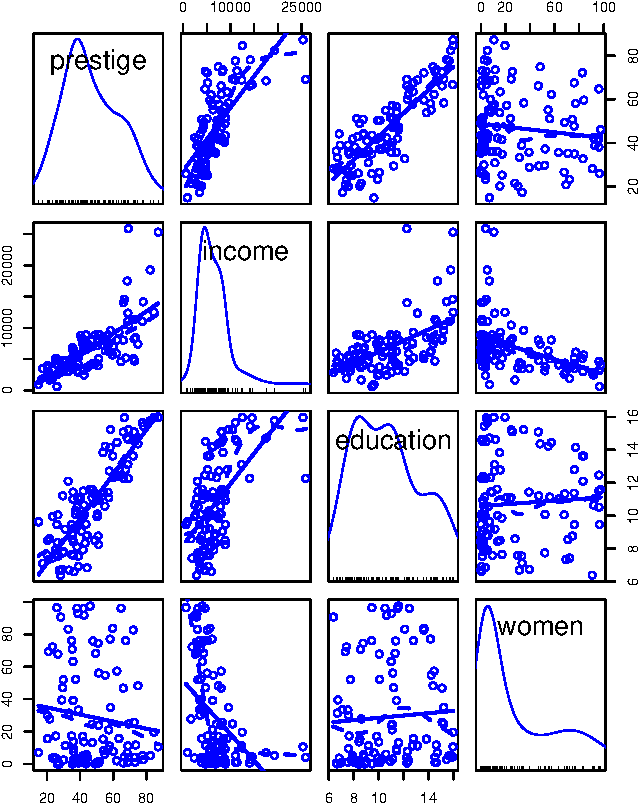
\includegraphics[width=1\linewidth]{JSS-article_files/figure-latex/scatterplot-matrix-1} 

}

\caption[Scatterplot matrix for the `Prestige` data]{Scatterplot matrix for the `Prestige` data.}\label{fig:scatterplot-matrix}
\end{figure}
\end{CodeChunk}

The \texttt{powerTransform()} function in the \textbf{car} package
transforms variables towards multivariate normality by a generalization
of Box and Cox's maximum-likelihood-like approach \citep{BoxCox:1964}.
Several ``families'' of power transformations can be used, including the
original Box-Cox family, simple powers (and roots), and two adaptations
of the Box-Cox family to data that may include negative values and
zeros: the Box-Cox-with-negatives family and the Yeo-Johnson family; see
\citet[Chap. 8]{Weisberg:2014}, and \citet[Chap. 3]{FoxWeisberg:2019}
for details. Because \texttt{women} has some zero values, we use the
Yeo-Johnson family:

\begin{CodeChunk}
\begin{CodeInput}
R> trans <- powerTransform( cbind(income, education, women) ~ 1,
+                          data=Prestige, family="yjPower")
R> summary(trans)
\end{CodeInput}
\begin{CodeOutput}
yjPower Transformations to Multinormality 
          Est Power Rounded Pwr Wald Lwr Bnd Wald Upr Bnd
income       0.2678        0.33       0.1051       0.4304
education    0.5162        1.00      -0.2822       1.3145
women        0.1630        0.16       0.0112       0.3149

 Likelihood ratio test that all transformation parameters are equal to 0
                               LRT df      pval
LR test, lambda = (0 0 0) 15.73879  3 0.0012827
\end{CodeOutput}
\end{CodeChunk}

We thus have evidence of the desirability of transforming
\texttt{income} (by the \(1/3\) power) and \texttt{women} (by the
\(0.16\) power---which is close to the ``0'' power, i.e., the log
transformation), but not \texttt{education}. Applying the ``rounded''
power transformations makes the predictors better-behaved:

\begin{CodeChunk}
\begin{CodeInput}
R> P <- Prestige[, c("prestige", "income", "education", "women")]
R> (lambdas <- trans$roundlam)
\end{CodeInput}
\begin{CodeOutput}
   income education     women 
0.3300000 1.0000000 0.1630182 
\end{CodeOutput}
\begin{CodeInput}
R> names(lambdas) <- c("income", "education", "women")
R> for (var in c("income", "education", "women")){
+   P[, var] <- yjPower(P[, var], lambda=lambdas[var])
+ }
R> summary(P)
\end{CodeInput}
\begin{CodeOutput}
    prestige         income        education          women      
 Min.   :14.80   Min.   :22.15   Min.   : 6.380   Min.   :0.000  
 1st Qu.:35.23   1st Qu.:44.17   1st Qu.: 8.445   1st Qu.:1.731  
 Median :43.60   Median :50.26   Median :10.540   Median :3.362  
 Mean   :46.83   Mean   :50.76   Mean   :10.738   Mean   :3.502  
 3rd Qu.:59.27   3rd Qu.:56.24   3rd Qu.:12.648   3rd Qu.:5.591  
 Max.   :87.20   Max.   :83.62   Max.   :15.970   Max.   :6.830  
\end{CodeOutput}
\begin{CodeInput}
R> scatterplotMatrix(~ prestige + income + education + women,
+                   data=P, smooth=list(spread=FALSE))
\end{CodeInput}
\begin{figure}

{\centering 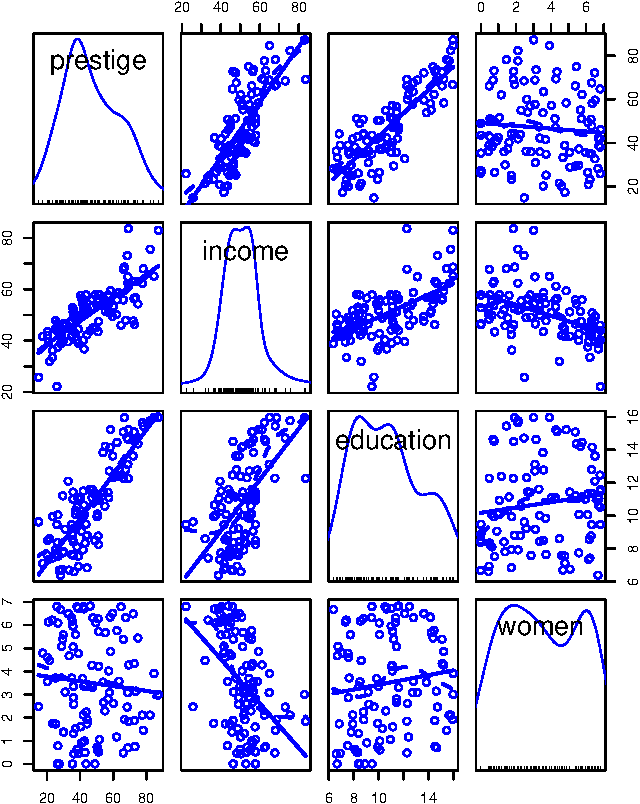
\includegraphics[width=1\linewidth]{JSS-article_files/figure-latex/transformed-predictors-1} 

}

\caption[Scatterplot matrix for the `Prestige` data with the predictors transformed]{Scatterplot matrix for the `Prestige` data with the predictors transformed.}\label{fig:transformed-predictors}
\end{figure}
\end{CodeChunk}

Comparing the MSE for the regressions with the original and transformed
predictors shows a advantage to the latter:

\begin{CodeChunk}
\begin{CodeInput}
R> m.pres <- lm(prestige ~ income + education + women, data=Prestige)
R> m.pres.trans <- lm(prestige ~ income + education + women, data=P)
R> mse(Prestige$prestige, fitted(m.pres))
\end{CodeInput}
\begin{CodeOutput}
[1] 59.15265
attr(,"casewise loss")
[1] "(y - yhat)^2"
\end{CodeOutput}
\begin{CodeInput}
R> mse(P$prestige, fitted(m.pres.trans))
\end{CodeInput}
\begin{CodeOutput}
[1] 50.60016
attr(,"casewise loss")
[1] "(y - yhat)^2"
\end{CodeOutput}
\end{CodeChunk}

Similarly, component+residual plots for the two regressions, produced by
the \texttt{crPlots()} function in the \textbf{car} package, suggest
that the partial relationship of \texttt{prestige} to \texttt{income} is
more nearly linear in the transformed data, but the transformation of
\texttt{women} fails to capture what appears to be a slight quadratic
partial relationship; the partial relationship of \texttt{prestige} to
\texttt{education} is close to linear in both regressions:

\begin{CodeChunk}
\begin{CodeInput}
R> crPlots(m.pres)
\end{CodeInput}
\begin{figure}

{\centering 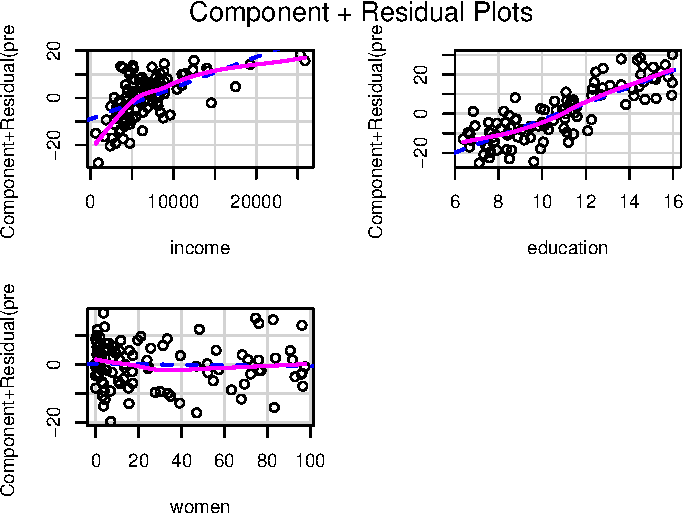
\includegraphics{JSS-article_files/figure-latex/CR-plots-untransformed-1} 

}

\caption[Component+residual plots for the `Prestige` regression with the original predictors]{Component+residual plots for the `Prestige` regression with the original predictors.}\label{fig:CR-plots-untransformed}
\end{figure}
\end{CodeChunk}

\begin{CodeChunk}
\begin{CodeInput}
R> crPlots(m.pres.trans)
\end{CodeInput}
\begin{figure}

{\centering 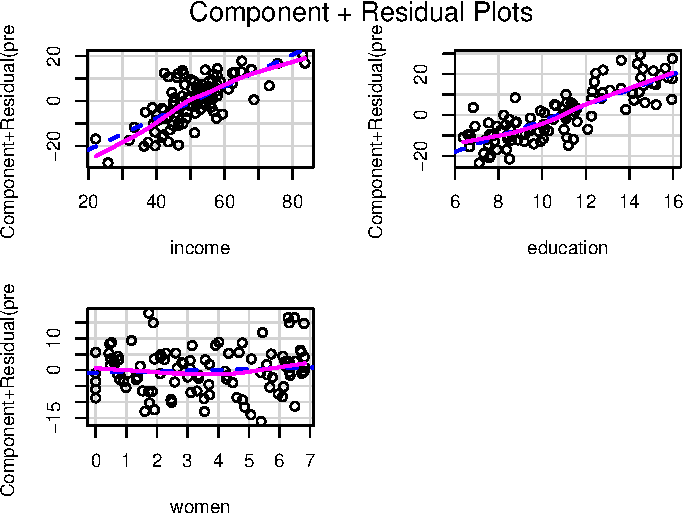
\includegraphics{JSS-article_files/figure-latex/CR-plots-transformed-1} 

}

\caption[Component+residual plots for the `Prestige` regression with transformed predictors]{Component+residual plots for the `Prestige` regression with transformed predictors.}\label{fig:CR-plots-transformed}
\end{figure}
\end{CodeChunk}

Having transformed the predictors towards multinormality, we now
consider whether there's evidence for transforming the response (using
\texttt{powerTransform()} for Box and Cox's original method), and we
discover that there's not:

\begin{CodeChunk}
\begin{CodeInput}
R> summary(powerTransform(m.pres.trans))
\end{CodeInput}
\begin{CodeOutput}
bcPower Transformation to Normality 
   Est Power Rounded Pwr Wald Lwr Bnd Wald Upr Bnd
Y1    1.0194           1       0.6773       1.3615

Likelihood ratio test that transformation parameter is equal to 0
 (log transformation)
                          LRT df       pval
LR test, lambda = (0) 32.2174  1 1.3785e-08

Likelihood ratio test that no transformation is needed
                             LRT df    pval
LR test, lambda = (1) 0.01238421  1 0.91139
\end{CodeOutput}
\end{CodeChunk}

The \texttt{selectTrans()} function in the \textbf{cv} package automates
the process of selecting predictor and response transformations. The
function takes a \texttt{data} set and ``working'' \texttt{model} as
arguments, along with the candidate \texttt{predictors} and
\texttt{response} for transformation, and the transformation
\texttt{family} to employ. If the \texttt{predictors} argument is
missing then only the response is transformed, and if the
\texttt{response} argument is missing, only the supplied predictors are
transformed. The default \texttt{family} for transforming the predictors
is \texttt{"bcPower"}---the original Box-Cox family---as is the default
\texttt{family.y} for transforming the response; here we specify
\texttt{family="yjPower} because of the zeros in \texttt{women}.
\texttt{selectTrans()} returns the result of applying a lack-of-fit
criterion to the model after the selected transformation is applied,
with the default \texttt{criterion=mse}:

\begin{CodeChunk}
\begin{CodeInput}
R> selectTrans(data=Prestige, model=m.pres,
+             predictors=c("income", "education", "women"),
+             response="prestige", family="yjPower")
\end{CodeInput}
\begin{CodeOutput}
[1] 50.60016
attr(,"casewise loss")
[1] "(y - yhat)^2"
\end{CodeOutput}
\end{CodeChunk}

\texttt{selectTrans()} also takes an optional \texttt{indices} argument,
making it suitable for doing computations on a subset of the data (i.e.,
a CV fold), and hence for use with \texttt{cvSelect()} (see
\texttt{?selectTrans} for details):

\begin{CodeChunk}
\begin{CodeInput}
R> cvs <- cvSelect(selectTrans, data=Prestige, model=m.pres, seed=1463,
+                 predictors=c("income", "education", "women"),
+                 response="prestige",
+                 family="yjPower")
\end{CodeInput}
\begin{CodeOutput}
R RNG seed set to 1463
\end{CodeOutput}
\begin{CodeInput}
R> cvs
\end{CodeInput}
\begin{CodeOutput}
10-Fold Cross Validation
cross-validation criterion = 54.4871
bias-adjusted cross-validation criterion = 54.30824
full-sample criterion = 50.60016 
\end{CodeOutput}
\begin{CodeInput}
R> cv(m.pres, seed=1463) # untransformed model with same folds
\end{CodeInput}
\begin{CodeOutput}
R RNG seed set to 1463
\end{CodeOutput}
\begin{CodeOutput}
10-Fold Cross Validation
method: Woodbury
criterion: mse
cross-validation criterion = 63.2926
bias-adjusted cross-validation criterion = 63.07251
full-sample criterion = 59.15265 
\end{CodeOutput}
\begin{CodeInput}
R> compareFolds(cvs)
\end{CodeInput}
\begin{CodeOutput}
        lam.education lam.income lam.women lambda
Fold 1          1.000      0.330     0.330      1
Fold 2          1.000      0.330     0.169      1
Fold 3          1.000      0.330     0.330      1
Fold 4          1.000      0.330     0.330      1
Fold 5          1.000      0.330     0.000      1
Fold 6          1.000      0.330     0.330      1
Fold 7          1.000      0.330     0.330      1
Fold 8          1.000      0.330     0.000      1
Fold 9          1.000      0.330     0.000      1
Fold 10         1.000      0.330     0.000      1
\end{CodeOutput}
\end{CodeChunk}

The results suggest that the predictive power of the transformed
regression is reliably greater than that of the untransformed regression
(though in both case, the cross-validated MSE is considerably higher
than the MSE computed for the whole data). Examining the selected
transformations for each fold reveals that the predictor
\texttt{education} and the response \texttt{prestige} are never
transformed; that the \(1/3\) power is selected for \texttt{income} in
all of the folds; and that the transformation selected for
\texttt{women} varies narrowly across the folds between the \(0\)th
power (i.e., log) and the \(1/3\) power.

\hypertarget{selecting-both-transformations-and-predictorsvenables}{%
\subsection[Selecting both transformations and
predictors]{\texorpdfstring{Selecting both transformations and
predictors\footnote{The presentation in the section benefits from an
  email conversation with Bill Venables, who of course isn't responsible
  for the use to which we've put his insightful remarks.}}{Selecting both transformations and predictors}}\label{selecting-both-transformations-and-predictorsvenables}}

As we mentioned, \citet[Sec. 7.10.2: ``The Wrong and Right Way to Do
Cross-validation'']{HastieTibshiraniFriedman:2009} explain that honest
cross-validation has to take account of model specification and
selection. Statistical modeling is at least partly a craft, and one
could imagine applying that craft to successive partial data sets, each
with a fold removed. The resulting procedure would be tedious, though
possibly worth the effort, but it would also be difficult to realize in
practice: After all, we can hardly erase our memory of statistical
modeling choices between analyzing partial data sets.

Alternatively, if we're able to automate the process of model selection,
then we can more realistically apply CV mechanically. That's what we did
in the preceding two sections, first for predictor selection and then
for selection of transformations in regression. In this section, we
consider the case where we both select variable transformations and then
proceed to select predictors. It's insufficient to apply these steps
sequentially, first, for example, using \texttt{cvSelect()} with
\texttt{selectTrans()} and then with \texttt{selectStepAIC()}; rather we
should apply the whole model-selection procedure with each fold omitted.
The \texttt{selectTransAndStepAIC()} function, also supplied by the
\textbf{cv} package, does exactly that.

To illustrate this process, we return to the \texttt{Auto} data set:

\begin{CodeChunk}
\begin{CodeInput}
R> summary(Auto)
\end{CodeInput}
\begin{CodeOutput}
      mpg          cylinders      displacement     horsepower        weight    
 Min.   : 9.00   Min.   :3.000   Min.   : 68.0   Min.   : 46.0   Min.   :1613  
 1st Qu.:17.00   1st Qu.:4.000   1st Qu.:105.0   1st Qu.: 75.0   1st Qu.:2225  
 Median :22.75   Median :4.000   Median :151.0   Median : 93.5   Median :2804  
 Mean   :23.45   Mean   :5.472   Mean   :194.4   Mean   :104.5   Mean   :2978  
 3rd Qu.:29.00   3rd Qu.:8.000   3rd Qu.:275.8   3rd Qu.:126.0   3rd Qu.:3615  
 Max.   :46.60   Max.   :8.000   Max.   :455.0   Max.   :230.0   Max.   :5140  
                                                                               
  acceleration        year           origin                      name    
 Min.   : 8.00   Min.   :70.00   Min.   :1.000   amc matador       :  5  
 1st Qu.:13.78   1st Qu.:73.00   1st Qu.:1.000   ford pinto        :  5  
 Median :15.50   Median :76.00   Median :1.000   toyota corolla    :  5  
 Mean   :15.54   Mean   :75.98   Mean   :1.577   amc gremlin       :  4  
 3rd Qu.:17.02   3rd Qu.:79.00   3rd Qu.:2.000   amc hornet        :  4  
 Max.   :24.80   Max.   :82.00   Max.   :3.000   chevrolet chevette:  4  
                                                 (Other)           :365  
\end{CodeOutput}
\begin{CodeInput}
R> xtabs(~ year, data=Auto)
\end{CodeInput}
\begin{CodeOutput}
year
70 71 72 73 74 75 76 77 78 79 80 81 82 
29 27 28 40 26 30 34 28 36 29 27 28 30 
\end{CodeOutput}
\begin{CodeInput}
R> xtabs(~ origin, data=Auto)
\end{CodeInput}
\begin{CodeOutput}
origin
  1   2   3 
245  68  79 
\end{CodeOutput}
\begin{CodeInput}
R> xtabs(~ cylinders, data=Auto)
\end{CodeInput}
\begin{CodeOutput}
cylinders
  3   4   5   6   8 
  4 199   3  83 103 
\end{CodeOutput}
\end{CodeChunk}

We previously used the \texttt{Auto} here in a preliminary example where
we employed CV to inform the selection of the order of a polynomial
regression of \texttt{mpg} on \texttt{horsepower}. Here, we consider
more generally the problem of predicting \texttt{mpg} from the other
variables in the \texttt{Auto} data. We begin with a bit of data
management, and then examine the pairwise relationships among the
numeric variables in the data set:

\begin{CodeChunk}
\begin{CodeInput}
R> Auto$cylinders <- factor(Auto$cylinders,
+                          labels=c("3.4", "3.4", "5.6", "5.6", "8"))
R> Auto$year <- as.factor(Auto$year)
R> Auto$origin <- factor(Auto$origin,
+                       labels=c("America", "Europe", "Japan"))
R> rownames(Auto) <- make.names(Auto$name, unique=TRUE)
R> Auto$name <- NULL
R> 
R> scatterplotMatrix(~ mpg + displacement + horsepower + weight + acceleration, 
+                   smooth=list(spread=FALSE), data=Auto)
\end{CodeInput}
\begin{figure}

{\centering 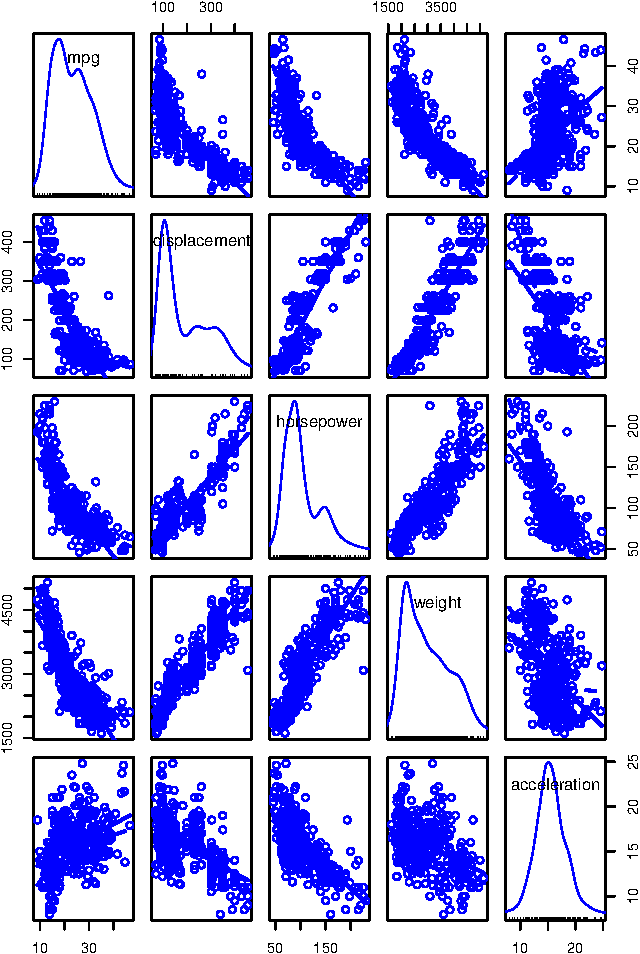
\includegraphics[width=1\linewidth]{JSS-article_files/figure-latex/Auto-explore-1} 

}

\caption[Scatterplot matrix for the numeric variables in the `Auto` data]{Scatterplot matrix for the numeric variables in the `Auto` data}\label{fig:Auto-explore}
\end{figure}
\end{CodeChunk}

A comment before we proceed: \texttt{origin} is clearly categorical and
so converting it to a factor is natural, but we could imagine treating
\texttt{cylinders} and \texttt{year} as numeric predictors. There are,
however, only 5 distinct values of \texttt{cylinders} (ranging from 3 to
8), but cars with 3 or 5 cylinders are rare. and none of the cars has 7
cylinders. There are similarly only 13 distinct years between 1970 and
1982 in the data, and the relationship between \texttt{mpg} and
\texttt{year} is difficult to characterize.\footnote{Of course, making
  the decision to treat \texttt{year} as a factor on this basis could be
  construed as cheating in the current context, which illustrates the
  difficulty of automating the whole model-selection process. It's
  rarely desirable, in our opinion, to forgo exploration of the data to
  ensure the purity of model validation. We believe, however, that it's
  still useful to automate as much of the process as we can to obtain a
  more realistic, if still biased, estimate of the predictive power of a
  model.} It's apparent that most these variables are positively skewed
and that many of the pairwise relationships among them are nonlinear.

We begin with a ``working model'' that specifies linear partial
relationships of the response to the numeric predictors:

\begin{CodeChunk}
\begin{CodeInput}
R> m.auto <- lm(mpg ~ ., data = Auto)
R> summary(m.auto)
\end{CodeInput}
\begin{CodeOutput}

Call:
lm(formula = mpg ~ ., data = Auto)

Residuals:
    Min      1Q  Median      3Q     Max 
-9.0064 -1.7450 -0.0917  1.5251 10.9504 

Coefficients:
               Estimate Std. Error t value Pr(>|t|)
(Intercept)  37.0341323  1.9693933  18.805  < 2e-16
cylinders5.6 -2.6029412  0.6552000  -3.973 8.54e-05
cylinders8   -0.5824578  1.1714516  -0.497 0.619335
displacement  0.0174253  0.0067340   2.588 0.010043
horsepower   -0.0413534  0.0133786  -3.091 0.002145
weight       -0.0055479  0.0006323  -8.774  < 2e-16
acceleration  0.0615272  0.0883132   0.697 0.486431
year71        0.9680584  0.8373899   1.156 0.248408
year72       -0.6014345  0.8251155  -0.729 0.466517
year73       -0.6876890  0.7402723  -0.929 0.353510
year74        1.3755758  0.8765000   1.569 0.117408
year75        0.9299288  0.8590716   1.082 0.279742
year76        1.5598929  0.8225051   1.897 0.058669
year77        2.9094161  0.8417285   3.456 0.000611
year78        3.1751976  0.7989396   3.974 8.48e-05
year79        5.0192987  0.8457587   5.935 6.76e-09
year80        9.0997634  0.8972933  10.141  < 2e-16
year81        6.6886597  0.8852181   7.556 3.28e-13
year82        8.0711248  0.8706683   9.270  < 2e-16
originEurope  2.0466642  0.5171236   3.958 9.07e-05
originJapan   2.1448874  0.5077169   4.225 3.02e-05

Residual standard error: 2.924 on 371 degrees of freedom
Multiple R-squared:  0.8668,    Adjusted R-squared:  0.8596 
F-statistic: 120.7 on 20 and 371 DF,  p-value: < 2.2e-16
\end{CodeOutput}
\begin{CodeInput}
R> Anova(m.auto)
\end{CodeInput}
\begin{CodeOutput}
Anova Table (Type II tests)

Response: mpg
             Sum Sq  Df F value    Pr(>F)
cylinders     292.3   2 17.0915 7.935e-08
displacement   57.3   1  6.6959  0.010043
horsepower     81.7   1  9.5544  0.002145
weight        658.3   1 76.9801 < 2.2e-16
acceleration    4.2   1  0.4854  0.486431
year         3016.8  12 29.3987 < 2.2e-16
origin        190.3   2 11.1287 2.024e-05
Residuals    3172.5 371                  
\end{CodeOutput}
\begin{CodeInput}
R> crPlots(m.auto)
\end{CodeInput}
\begin{figure}

{\centering 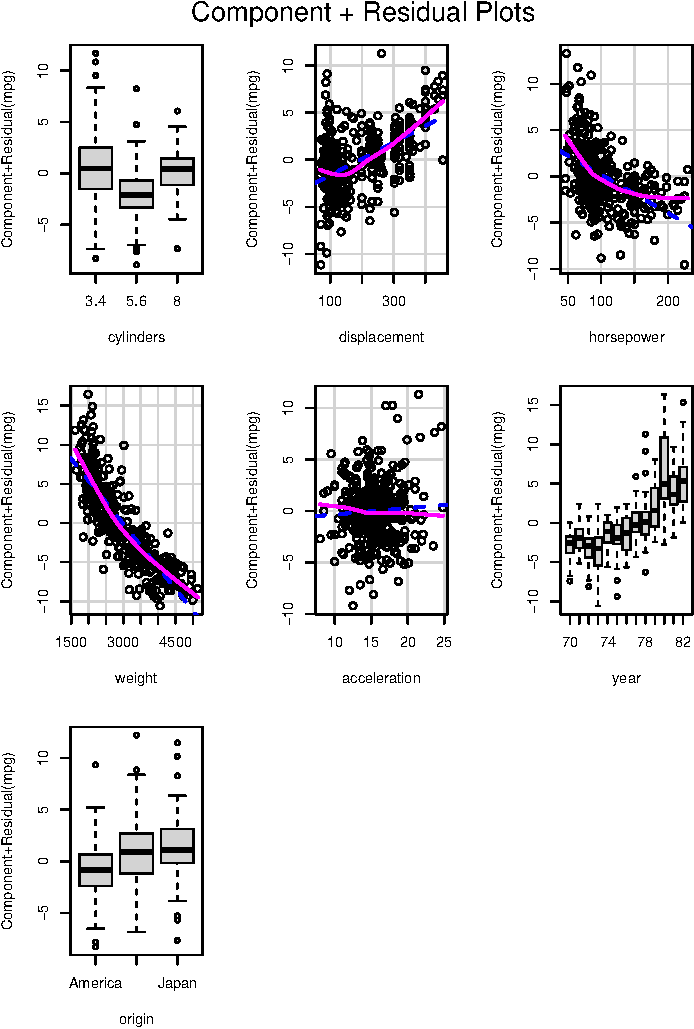
\includegraphics[width=1\linewidth]{JSS-article_files/figure-latex/Auto-working-model-1} 

}

\caption[Component+residual plots for the working model fit to the `Auto` data]{Component+residual plots for the working model fit to the `Auto` data}\label{fig:Auto-working-model}
\end{figure}
\end{CodeChunk}

The component+residual plots, created with the \texttt{crPlots()}
function in the previously loaded \textbf{car} package, clearly reveal
the inadequacy of the model.

We proceed to transform the numeric predictors towards multi-normality:

\begin{CodeChunk}
\begin{CodeInput}
R> num.predictors <- c("displacement", "horsepower", "weight", "acceleration")
R> tr.x <- powerTransform(Auto[, num.predictors])
R> summary(tr.x)
\end{CodeInput}
\begin{CodeOutput}
bcPower Transformations to Multinormality 
             Est Power Rounded Pwr Wald Lwr Bnd Wald Upr Bnd
displacement   -0.0509           0      -0.2082       0.1065
horsepower     -0.1249           0      -0.2693       0.0194
weight         -0.0870           0      -0.2948       0.1208
acceleration    0.3061           0      -0.0255       0.6376

Likelihood ratio test that transformation parameters are equal to 0
 (all log transformations)
                                 LRT df    pval
LR test, lambda = (0 0 0 0) 4.872911  4 0.30059

Likelihood ratio test that no transformations are needed
                                 LRT df       pval
LR test, lambda = (1 1 1 1) 390.0777  4 < 2.22e-16
\end{CodeOutput}
\end{CodeChunk}

We then apply the (rounded) transformations---all, as it turns out,
logs---to the data and re-estimate the model:

\begin{CodeChunk}
\begin{CodeInput}
R> A <- Auto
R> powers <- tr.x$roundlam
R> for (pred in num.predictors){
+   A[, pred] <- bcPower(A[, pred], lambda=powers[pred])
+ }
R> head(A)
\end{CodeInput}
\begin{CodeOutput}
                          mpg cylinders displacement horsepower   weight
chevrolet.chevelle.malibu  18         8     5.726848   4.867534 8.161660
buick.skylark.320          15         8     5.857933   5.105945 8.214194
plymouth.satellite         18         8     5.762051   5.010635 8.142063
amc.rebel.sst              16         8     5.717028   5.010635 8.141190
ford.torino                17         8     5.710427   4.941642 8.145840
ford.galaxie.500           15         8     6.061457   5.288267 8.375860
                          acceleration year  origin
chevrolet.chevelle.malibu     2.484907   70 America
buick.skylark.320             2.442347   70 America
plymouth.satellite            2.397895   70 America
amc.rebel.sst                 2.484907   70 America
ford.torino                   2.351375   70 America
ford.galaxie.500              2.302585   70 America
\end{CodeOutput}
\begin{CodeInput}
R> m <- update(m.auto, data=A)
\end{CodeInput}
\end{CodeChunk}

Finally, we perform Box-Cox regression to transform the response (also
obtaining a log transformation):

\begin{CodeChunk}
\begin{CodeInput}
R> summary(powerTransform(m))
\end{CodeInput}
\begin{CodeOutput}
bcPower Transformation to Normality 
   Est Power Rounded Pwr Wald Lwr Bnd Wald Upr Bnd
Y1    0.0024           0      -0.1607       0.1654

Likelihood ratio test that transformation parameter is equal to 0
 (log transformation)
                               LRT df    pval
LR test, lambda = (0) 0.0008015428  1 0.97741

Likelihood ratio test that no transformation is needed
                           LRT df       pval
LR test, lambda = (1) 124.1307  1 < 2.22e-16
\end{CodeOutput}
\begin{CodeInput}
R> m <- update(m, log(mpg) ~ .)
R> summary(m)
\end{CodeInput}
\begin{CodeOutput}

Call:
lm(formula = log(mpg) ~ cylinders + displacement + horsepower + 
    weight + acceleration + year + origin, data = A)

Residuals:
     Min       1Q   Median       3Q      Max 
-0.33412 -0.05774  0.00410  0.06072  0.38081 

Coefficients:
             Estimate Std. Error t value Pr(>|t|)
(Intercept)   8.89652    0.35822  24.835  < 2e-16
cylinders5.6 -0.06355    0.02574  -2.469   0.0140
cylinders8   -0.07691    0.03900  -1.972   0.0493
displacement  0.02799    0.05146   0.544   0.5868
horsepower   -0.29010    0.05631  -5.152 4.20e-07
weight       -0.54274    0.08193  -6.624 1.23e-10
acceleration -0.14214    0.05630  -2.525   0.0120
year71        0.02505    0.02891   0.866   0.3869
year72       -0.01680    0.02894  -0.580   0.5620
year73       -0.04257    0.02602  -1.636   0.1026
year74        0.04932    0.03041   1.622   0.1056
year75        0.04715    0.02959   1.594   0.1118
year76        0.07087    0.02845   2.491   0.0132
year77        0.13241    0.02927   4.523 8.21e-06
year78        0.14472    0.02777   5.211 3.13e-07
year79        0.23354    0.02921   7.994 1.67e-14
year80        0.32381    0.03170  10.216  < 2e-16
year81        0.25655    0.03094   8.291 2.10e-15
year82        0.30756    0.03036  10.131  < 2e-16
originEurope  0.04921    0.01955   2.518   0.0122
originJapan   0.04409    0.01947   2.265   0.0241

Residual standard error: 0.1043 on 371 degrees of freedom
Multiple R-squared:  0.9108,    Adjusted R-squared:  0.906 
F-statistic: 189.4 on 20 and 371 DF,  p-value: < 2.2e-16
\end{CodeOutput}
\begin{CodeInput}
R> Anova(m)
\end{CodeInput}
\begin{CodeOutput}
Anova Table (Type II tests)

Response: log(mpg)
             Sum Sq  Df F value    Pr(>F)
cylinders    0.0663   2  3.0521   0.04845
displacement 0.0032   1  0.2959   0.58679
horsepower   0.2885   1 26.5420 4.198e-07
weight       0.4769   1 43.8805 1.229e-10
acceleration 0.0693   1  6.3745   0.01199
year         4.4521  12 34.1339 < 2.2e-16
origin       0.0807   2  3.7128   0.02532
Residuals    4.0325 371                  
\end{CodeOutput}
\end{CodeChunk}

The transformed numeric variables are much better-behaved:

\begin{CodeChunk}
\begin{CodeInput}
R> scatterplotMatrix(~ log(mpg) + displacement + horsepower + weight 
+                   + acceleration, 
+                   smooth=list(spread=FALSE), data=A)
\end{CodeInput}
\begin{figure}

{\centering 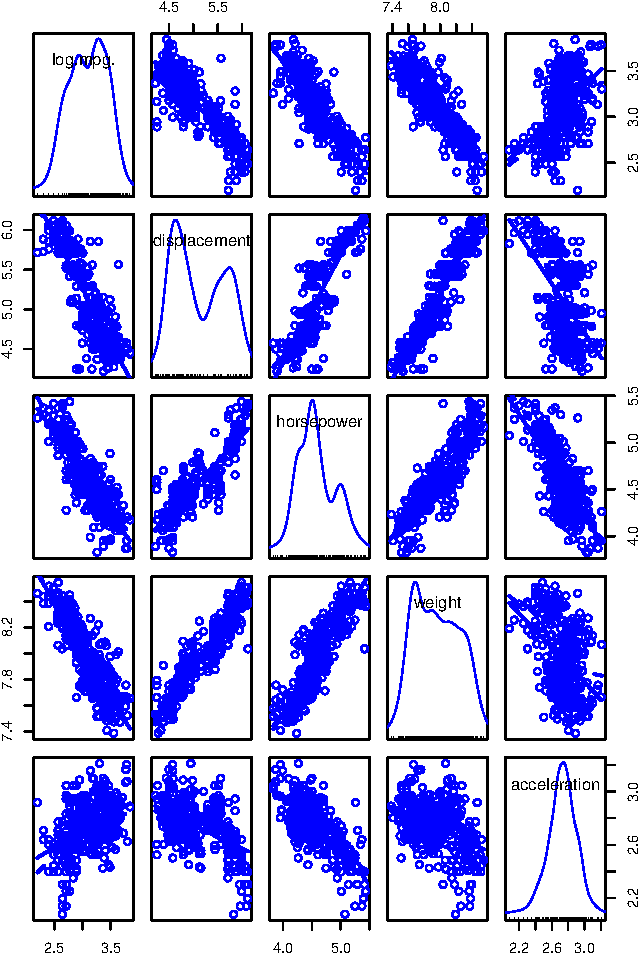
\includegraphics[width=1\linewidth]{JSS-article_files/figure-latex/Auto-transformed-scatterplot-matrix-1} 

}

\caption[Scatterplot matrix for the transformed numeric variables in the `Auto` data]{Scatterplot matrix for the transformed numeric variables in the `Auto` data}\label{fig:Auto-transformed-scatterplot-matrix}
\end{figure}
\end{CodeChunk}

And the partial relationships in the model fit to the transformed data
are much more nearly linear:

\begin{CodeChunk}
\begin{CodeInput}
R> crPlots(m)
\end{CodeInput}
\begin{figure}

{\centering 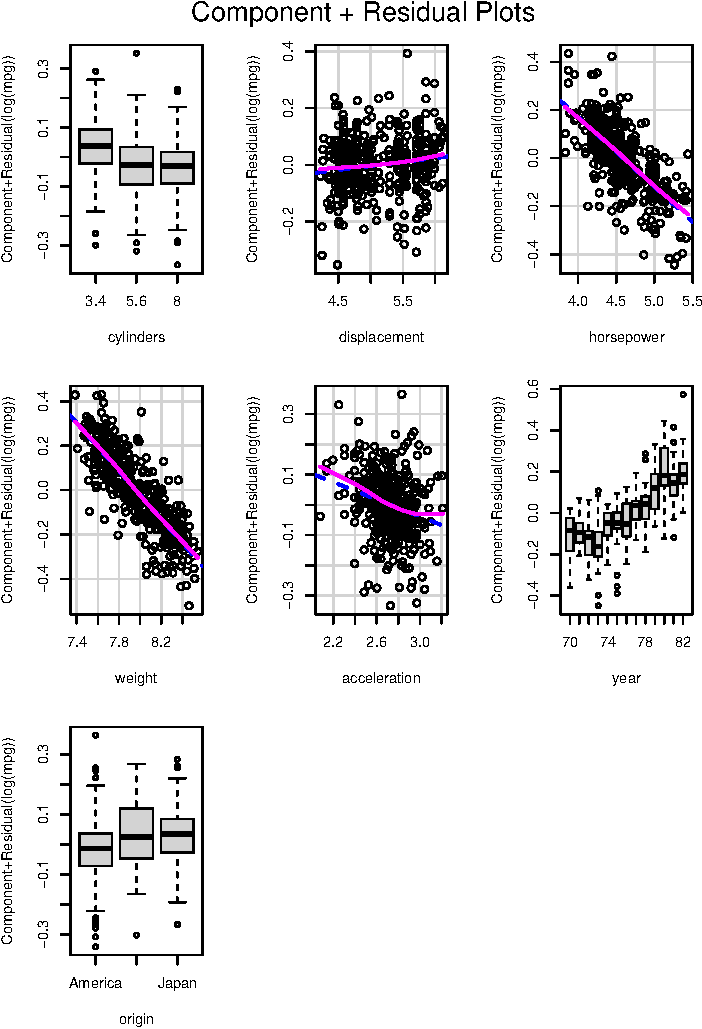
\includegraphics[width=1\linewidth]{JSS-article_files/figure-latex/Auto-CR-plots-transformed-1} 

}

\caption[Component+residual plots for the model fit to the transformed `Auto` data]{Component+residual plots for the model fit to the transformed `Auto` data}\label{fig:Auto-CR-plots-transformed}
\end{figure}
\end{CodeChunk}

Having transformed both the numeric predictors and the response, we
proceed to use the \texttt{stepAIC()} function in the \textbf{MASS}
package to perform predictor selection, employing the BIC
model-selection criterion (by setting the \texttt{k} argument of
\texttt{stepAIC()} to \(\log(n)\)):

\begin{CodeChunk}
\begin{CodeInput}
R> m.step <- stepAIC(m, k=log(nrow(A)), trace=FALSE)
R> summary(m.step)
\end{CodeInput}
\begin{CodeOutput}

Call:
lm(formula = log(mpg) ~ horsepower + weight + acceleration + 
    year + origin, data = A)

Residuals:
     Min       1Q   Median       3Q      Max 
-0.35230 -0.05682  0.00677  0.06741  0.35861 

Coefficients:
              Estimate Std. Error t value Pr(>|t|)
(Intercept)   9.434594   0.261529  36.075  < 2e-16
horsepower   -0.276254   0.056143  -4.921 1.30e-06
weight       -0.609071   0.056003 -10.876  < 2e-16
acceleration -0.131380   0.053195  -2.470  0.01397
year71        0.027984   0.028936   0.967  0.33412
year72       -0.007111   0.028446  -0.250  0.80274
year73       -0.039529   0.026014  -1.520  0.12947
year74        0.052752   0.029986   1.759  0.07936
year75        0.053199   0.029280   1.817  0.07004
year76        0.074317   0.028212   2.634  0.00878
year77        0.137931   0.028875   4.777 2.56e-06
year78        0.145876   0.027529   5.299 1.99e-07
year79        0.236036   0.029080   8.117 6.99e-15
year80        0.335274   0.031148  10.764  < 2e-16
year81        0.262872   0.030555   8.603  < 2e-16
year82        0.323391   0.029608  10.922  < 2e-16
originEurope  0.055818   0.016785   3.326  0.00097
originJapan   0.043554   0.017479   2.492  0.01314

Residual standard error: 0.1049 on 374 degrees of freedom
Multiple R-squared:  0.909, Adjusted R-squared:  0.9049 
F-statistic: 219.8 on 17 and 374 DF,  p-value: < 2.2e-16
\end{CodeOutput}
\begin{CodeInput}
R> Anova(m.step)
\end{CodeInput}
\begin{CodeOutput}
Anova Table (Type II tests)

Response: log(mpg)
             Sum Sq  Df  F value    Pr(>F)
horsepower   0.2663   1  24.2120 1.296e-06
weight       1.3010   1 118.2805 < 2.2e-16
acceleration 0.0671   1   6.0998  0.013965
year         4.7589  12  36.0549 < 2.2e-16
origin       0.1366   2   6.2090  0.002225
Residuals    4.1137 374                   
\end{CodeOutput}
\end{CodeChunk}

The selected model includes three of the numeric predictors,
\texttt{horsepower}, \texttt{weight}, and \texttt{acceleration}, along
with the factors \texttt{year} and \texttt{origin}. We can calculate the
MSE for this model, but we expect that the result will be optimistic
because we used the whole data to help specify the model

\begin{CodeChunk}
\begin{CodeInput}
R> mse(Auto$mpg, exp(fitted(m.step)))
\end{CodeInput}
\begin{CodeOutput}
[1] 6.512144
attr(,"casewise loss")
[1] "(y - yhat)^2"
\end{CodeOutput}
\end{CodeChunk}

This is considerably smaller than the MSE for the original working
model:

\begin{CodeChunk}
\begin{CodeInput}
R> mse(Auto$mpg, fitted(m.auto))
\end{CodeInput}
\begin{CodeOutput}
[1] 8.093171
attr(,"casewise loss")
[1] "(y - yhat)^2"
\end{CodeOutput}
\end{CodeChunk}

A perhaps subtle point is that we compute the MSE for the selected model
on the original \texttt{mpg} response scale rather than the log scale,
so as to make the selected model comparable to the working model. That's
slightly uncomfortable given the skewed distribution of \texttt{mpg}. An
alternative is to use the median absolute error instead of the
mean-squared error, employing the \texttt{medAbsErr()} function from the
\textbf{cv} package:

\begin{CodeChunk}
\begin{CodeInput}
R> medAbsErr(Auto$mpg, exp(fitted(m.step)))
\end{CodeInput}
\begin{CodeOutput}
[1] 1.339604
\end{CodeOutput}
\begin{CodeInput}
R> medAbsErr(Auto$mpg, fitted(m.auto))
\end{CodeInput}
\begin{CodeOutput}
[1] 1.666121
\end{CodeOutput}
\end{CodeChunk}

Now let's use \texttt{cvSelect()} with \texttt{selectTransAndStepAIC()}
to automate and cross-validate the whole model-specification process:

\begin{CodeChunk}
\begin{CodeInput}
R> num.predictors
\end{CodeInput}
\begin{CodeOutput}
[1] "displacement" "horsepower"   "weight"       "acceleration"
\end{CodeOutput}
\begin{CodeInput}
R> cvs <- cvSelect(selectTransStepAIC, data=Auto, seed=76692, model=m.auto,
+                 predictors=num.predictors,
+                 response="mpg", AIC=FALSE, criterion=medAbsErr)
\end{CodeInput}
\begin{CodeOutput}
R RNG seed set to 76692
\end{CodeOutput}
\begin{CodeInput}
R> cvs
\end{CodeInput}
\begin{CodeOutput}
10-Fold Cross Validation
cross-validation criterion = 1.495075
full-sample criterion = 1.339604 
\end{CodeOutput}
\begin{CodeInput}
R> compareFolds(cvs)
\end{CodeInput}
\begin{CodeOutput}
        (Intercept) horsepower lam.acceleration lam.displacement lam.horsepower
Fold 1      9.71384   -0.17408          0.50000          0.00000        0.00000
Fold 2      9.21713   -0.31480          0.00000          0.00000        0.00000
Fold 3      9.61824   -0.19248          0.00000          0.00000        0.00000
Fold 4      8.69910   -0.25523          0.50000          0.00000        0.00000
Fold 5      9.14403   -0.14934          0.00000          0.00000        0.00000
Fold 6      9.63481   -0.16739          0.50000          0.00000        0.00000
Fold 7      9.98933   -0.36847          0.00000          0.00000       -0.15447
Fold 8      9.06301   -0.29721          0.00000          0.00000        0.00000
Fold 9      8.88315   -0.22684          0.00000          0.00000        0.00000
Fold 10     9.61727   -0.17086          0.00000          0.00000        0.00000
        lam.weight   lambda   weight   year71   year72   year73   year74
Fold 1     0.00000  0.00000 -0.74636  0.03764 -0.00327 -0.02477  0.05606
Fold 2     0.00000  0.00000 -0.47728  0.02173 -0.01488 -0.03770  0.04312
Fold 3     0.00000  0.00000 -0.72085  0.01128 -0.02569 -0.03872  0.05187
Fold 4     0.00000  0.00000 -0.53846  0.02153 -0.02922 -0.05181  0.04136
Fold 5     0.00000  0.00000 -0.69081  0.02531 -0.01062 -0.04625  0.05039
Fold 6     0.00000  0.00000 -0.74049  0.02456  0.00759 -0.03412  0.06266
Fold 7     0.00000  0.00000 -0.72843  0.02532 -0.01271 -0.04144  0.04568
Fold 8     0.00000  0.00000 -0.46392  0.02702 -0.02041 -0.05605  0.04437
Fold 9     0.00000  0.00000 -0.47136  0.00860 -0.03620 -0.04835  0.01906
Fold 10    0.00000  0.00000 -0.73550  0.02937 -0.00899 -0.03814  0.05408
          year75   year76   year77   year78   year79   year80   year81   year82
Fold 1   0.07080  0.07250  0.14420  0.14281  0.23266  0.35127  0.25635  0.30546
Fold 2   0.04031  0.06718  0.13094  0.14917  0.21871  0.33192  0.26196  0.30943
Fold 3   0.03837  0.06399  0.11593  0.12601  0.20499  0.32821  0.24478  0.29204
Fold 4   0.04072  0.05537  0.12292  0.14083  0.22878  0.32947  0.25140  0.27248
Fold 5   0.05596  0.07044  0.13356  0.14724  0.24675  0.33331  0.26938  0.32594
Fold 6   0.06940  0.07769  0.14211  0.14647  0.23532  0.34761  0.26737  0.33062
Fold 7   0.03614  0.07385  0.12976  0.14040  0.23976  0.33998  0.27652  0.30659
Fold 8   0.06573  0.08135  0.13158  0.13987  0.23011  0.32880  0.25886  0.30538
Fold 9   0.03018  0.05846  0.10536  0.11722  0.20665  0.31533  0.23352  0.29375
Fold 10  0.04881  0.07862  0.14101  0.14313  0.23258  0.35649  0.26214  0.32421
        acceleration displacement cylinders5.6 cylinders8 originEurope
Fold 1                                                                
Fold 2      -0.18909     -0.09197                                     
Fold 3                                                                
Fold 4      -0.03484                  -0.09080   -0.10909             
Fold 5                                                         0.06261
Fold 6                                                                
Fold 7                                                                
Fold 8      -0.17676     -0.10542                                     
Fold 9      -0.14514     -0.13452                                     
Fold 10                                                               
        originJapan
Fold 1             
Fold 2             
Fold 3             
Fold 4             
Fold 5         0.04
Fold 6             
Fold 7             
Fold 8             
Fold 9             
Fold 10            
\end{CodeOutput}
\end{CodeChunk}

Here, as for \texttt{selectTrans()}, the \texttt{predictors} and
\texttt{response} arguments specify candidate variables for
transformation, and \texttt{AIC=FALSE} uses the BIC for model selection.
The starting model, \texttt{m.auto}, is the working model fit to the
\texttt{Auto} data. The CV criterion isn't bias-adjusted because median
absolute error isn't a mean of casewise error components.

Some noteworthy points:

\begin{itemize}
\tightlist
\item
  \texttt{selectTransStepAIC()} automatically computes CV cost criteria,
  here the median absolute error, on the untransformed response scale.
\item
  The estimate of the median absolute error that we obtain by
  cross-validating the whole model-specification process is a little
  larger than the median absolute error computed for the model we fit to
  the \texttt{Auto} data separately selecting transformations of the
  predictors and the response and then selecting predictors for the
  whole data set.
\item
  When we look at the transformations and predictors selected with each
  of the 10 folds omitted (i.e., the output of \texttt{compareFolds()}),
  we see that there is little uncertainty in choosing variable
  transformations (the \texttt{lam.*}s for the \(x\)s and
  \texttt{lambda} for \(y\) in the output), but considerably more
  uncertainty in subsequently selecting predictors: \texttt{horsepower},
  \texttt{weight}, and \texttt{year} are always included among the
  selected predictors; \texttt{acceleration} and \texttt{displacement}
  are each included respectively in 4 and 3 of 10 selected models; and
  \texttt{cylinders} and \texttt{origin} are each included in only 1 of
  10 models. Recall that when we selected predictors for the full data,
  we obtained a model with \texttt{horsepower}, \texttt{weight},
  \texttt{acceleration}, \texttt{year}, and \texttt{origin}.
\end{itemize}

\hypertarget{parallel-computations}{%
\section{Parallel computations}\label{parallel-computations}}

The CV functions in the \textbf{cv} package are all capable of
performing parallel computations by setting the \texttt{ncores} argument
(specifying the number of computer cores to be used) to a number
\textgreater{} \texttt{1} (which is the default). Parallel computation
can be advantageous for large problems, reducing the execution time of
the program.

To illustrate, let's time model selection in Mroz's logistic regression,
repeating the computation as performed previously and then doing it in
parallel using 2 cores:

\begin{CodeChunk}
\begin{CodeInput}
R> system.time(m.mroz.sel.cv <- cvSelect(selectStepAIC, Mroz,
+                           seed=6681,
+                           criterion=BayesRule,
+                           model=m.mroz,
+                           AIC=FALSE))
\end{CodeInput}
\begin{CodeOutput}
R RNG seed set to 6681
\end{CodeOutput}
\begin{CodeOutput}
   user  system elapsed 
  0.249   0.004   0.253 
\end{CodeOutput}
\begin{CodeInput}
R> system.time(m.mroz.sel.cv.p <- cvSelect(selectStepAIC, Mroz,
+                           seed=6681,
+                           criterion=BayesRule,
+                           model=m.mroz,
+                           AIC=FALSE,
+                           ncores=2))
\end{CodeInput}
\begin{CodeOutput}
R RNG seed set to 6681
\end{CodeOutput}
\begin{CodeOutput}
   user  system elapsed 
  0.035   0.004   0.949 
\end{CodeOutput}
\begin{CodeInput}
R> all.equal(m.mroz.sel.cv, m.mroz.sel.cv.p)
\end{CodeInput}
\begin{CodeOutput}
[1] TRUE
\end{CodeOutput}
\end{CodeChunk}

In this small problem, the parallel computation is actually
\emph{slower}, because there is an overhead cost to parallelization, but
we can see that it produces the same result as before.

\hypertarget{extending-the-cv-package}{%
\section{Extending the cv package}\label{extending-the-cv-package}}

The \textbf{cv} package is designed to be extensible in several
directions. In this vignette, we discuss three kinds of extensions,
ordered by increasing general complexity: (1) adding a cross-validation
cost criterion; (2) adding a model class that's not directly
accommodated by the \texttt{cv()} default method or by another directly
inherited method, with separate consideration of mixed-effects models;
and (3) adding a new model-selection procedure suitable for use with
\texttt{selectModel()}.

\hypertarget{adding-a-cost-criterion}{%
\subsection{Adding a cost criterion}\label{adding-a-cost-criterion}}

A cost criterion suitable for use with \texttt{cv()} or
\texttt{cvSelect()} should take two arguments, \texttt{y} (the observed
response vector) and \texttt{yhat} (a vector of fitted or predicted
response values), and return a numeric index of lack of fit. The
\textbf{cv} package supplies several such criteria:
\texttt{mse(y,\ yhat)}, which returns the mean-squared prediction error
for a numeric response; \texttt{rmse(y,\ yhat)}, which returns the
(square-)root mean-squared error; \texttt{medAbsErr(y,\ yhat)}, which
returns the median absolute error; and \texttt{BayesRule(y,\ yhat)} (and
its non-error-checking version, \texttt{BayesRule2(y,\ yhat))}, suitable
for use with a binary regression model, where \texttt{y} is the binary
response coded \texttt{0} for a ``failure'' or \texttt{1} for a
``success''; where \texttt{yhat} is the predicted probability of
success; and where the proportion of \emph{incorrectly} classified cases
is returned.

To illustrate using a different prediction cost criterion, we'll base a
cost criterion on the area under the receiver operating characteristic
(``ROC'') curve for a logistic regression. The ROC curve is a graphical
representation of the classification power of a binary regression model,
and the area under the ROC curve (``AUC''), which varies from 0 to 1, is
a common summary measure based on the ROC
\citep[see][]{Wikipedia-ROC:2023}. The \textbf{Metrics} package
\citep{HamnerFrasco:2018} includes a variety of measures useful for
model selection, including an \texttt{auc()} function. We convert the
AUC into a cost measure by taking its complement:

\begin{CodeChunk}
\begin{CodeInput}
R> AUCcomp <- function(y, yhat) 1 - Metrics::auc(y, yhat)
\end{CodeInput}
\end{CodeChunk}

We then apply \texttt{AUCcomp()} to the the Mroz logistic regression
discussed in the main \textbf{cv} package vignette, which we reproduce
here, using the \texttt{Mroz} data frame from the \textbf{carData}
package \citep{FoxWeisberg:2019}:

\begin{CodeChunk}
\begin{CodeInput}
R> data("Mroz", package="carData")
R> m.mroz <- glm(lfp ~ ., data=Mroz, family=binomial)
R> summary(m.mroz)
\end{CodeInput}
\begin{CodeOutput}

Call:
glm(formula = lfp ~ ., family = binomial, data = Mroz)

Coefficients:
             Estimate Std. Error z value Pr(>|z|)
(Intercept)  3.182140   0.644375   4.938 7.88e-07
k5          -1.462913   0.197001  -7.426 1.12e-13
k618        -0.064571   0.068001  -0.950 0.342337
age         -0.062871   0.012783  -4.918 8.73e-07
wcyes        0.807274   0.229980   3.510 0.000448
hcyes        0.111734   0.206040   0.542 0.587618
lwg          0.604693   0.150818   4.009 6.09e-05
inc         -0.034446   0.008208  -4.196 2.71e-05

(Dispersion parameter for binomial family taken to be 1)

    Null deviance: 1029.75  on 752  degrees of freedom
Residual deviance:  905.27  on 745  degrees of freedom
AIC: 921.27

Number of Fisher Scoring iterations: 4
\end{CodeOutput}
\begin{CodeInput}
R> AUCcomp(with(Mroz, as.numeric(lfp == "yes")), fitted(m.mroz))
\end{CodeInput}
\begin{CodeOutput}
[1] 0.2636161
\end{CodeOutput}
\end{CodeChunk}

Cross-validating this cost measure is straightforward:

\begin{CodeChunk}
\begin{CodeInput}
R> library("cv")
R> cv(m.mroz, criterion=AUCcomp, seed=3639)
\end{CodeInput}
\begin{CodeOutput}
R RNG seed set to 3639
\end{CodeOutput}
\begin{CodeOutput}
10-Fold Cross Validation
method: exact
criterion: AUCcomp
cross-validation criterion = 0.2747088
full-sample criterion = 0.2636161 
\end{CodeOutput}
\end{CodeChunk}

As expected, the cross-validated complement to the AUC is somewhat less
optimistic than the criterion computed from the model fit to the whole
data set.

As we explain in the vignette ``Cross-validation of regression models,''
the \texttt{cv()} function differentiates between CV criteria that are
averages of casewise components and criteria that are not. Computation
of bias corrections and confidence intervals is limited to the former.
We show in the appendix to this vignette that the AUC, and hence its
complement, cannot be expressed as averages of casewise components.

\texttt{cv()} looks for a \texttt{"casewise\ loss"} attribute of the
value returned by a CV criterion function. If this attribute exists,
then the criterion is treated as the mean of casewise components, and
\texttt{cv()} uses the unexported function \texttt{getLossFn()} to
construct a function that returns the casewise components of the
criterion.

We illustrate with the \texttt{mse()}:

\begin{CodeChunk}
\begin{CodeInput}
R> mse
\end{CodeInput}
\begin{CodeOutput}
 [1] 23.94366 18.98477 18.94499 18.87633 18.42697 18.24065 18.07817 18.06613
 [9] 18.02697 18.00953
\end{CodeOutput}
\begin{CodeInput}
R> cv:::getLossFn(mse(rnorm(100), rnorm(100)))
\end{CodeInput}
\begin{CodeOutput}
function (y, yhat) 
{
    (y - yhat)^2
}
<environment: 0x12bdf3978>
\end{CodeOutput}
\end{CodeChunk}

For this scheme to work, the ``casewise loss'' attribute must be a
character string (or vector of character strings), here
\texttt{"(y\ -\ yhat)\^{}2"}, that evaluates to an expression that is a
function of \texttt{y} and \texttt{yhat}, and that computes the vector
of casewise components of the CV criterion.

\hypertarget{adding-a-model-class-not-covered-by-the-default-cv-method}{%
\subsection{Adding a model class not covered by the default cv()
method}\label{adding-a-model-class-not-covered-by-the-default-cv-method}}

\hypertarget{independently-sampled-cases}{%
\subsubsection{Independently sampled
cases}\label{independently-sampled-cases}}

Suppose that we want to cross-validate a multinomial logistic regression
model fit by the \texttt{multinom()} function in the \textbf{nnet}
package \citep{VenablesRipley:2002}. We borrow an example from
\citet[Sec. 14.2.1]{Fox:2016}, with data from the British Election Panel
Study on vote choice in the 2001 British election. Data for the example
are in the \texttt{BEPS} data frame in the \textbf{carData} package:

\begin{CodeChunk}
\begin{CodeInput}
R> data("BEPS", package="carData")
R> head(BEPS)
\end{CodeInput}
\begin{CodeOutput}
              vote age economic.cond.national economic.cond.household Blair
1 Liberal Democrat  43                      3                       3     4
2           Labour  36                      4                       4     4
3           Labour  35                      4                       4     5
4           Labour  24                      4                       2     2
5           Labour  41                      2                       2     1
6           Labour  47                      3                       4     4
  Hague Kennedy Europe political.knowledge gender
1     1       4      2                   2 female
2     4       4      5                   2   male
3     2       3      3                   2   male
4     1       3      4                   0 female
5     1       4      6                   2   male
6     4       2      4                   2   male
\end{CodeOutput}
\end{CodeChunk}

The polytomous (multi-category) response variable is \texttt{vote}, a
factor with levels \texttt{"Conservative"}, \texttt{"Labour"}, and
\texttt{"Liberal\ Democrat"}. The predictors of \texttt{vote} are:

\begin{itemize}
\tightlist
\item
  \texttt{age}, in years;
\item
  \texttt{econ.cond.national} and \texttt{econ.cond.household}, the
  respondent's ratings of the state of the economy, on 1 to 5 scales.
\item
  \texttt{Blair}, \texttt{Hague}, and \texttt{Kennedy}, ratings of the
  leaders of the Labour, Conservative, and Liberal Democratic parties,
  on 1 to 5 scales.
\item
  \texttt{Europe}, an 11-point scale on attitude towards European
  integration, with high scores representing ``Euro-skepticism.''
\item
  \texttt{political.knowledge}, knowledge of the parties' positions on
  European integration, with scores from 0 to 3.
\item
  \texttt{gender}, \texttt{"female"} or \texttt{"male"}.
\end{itemize}

The model fit to the data includes an interaction between
\texttt{Europe} and \texttt{political.knowledge}; the other predictors
enter the model additively:

\begin{CodeChunk}
\begin{CodeInput}
R> library("nnet")
R> m.beps <- multinom(vote ~ age + gender + economic.cond.national +
+                        economic.cond.household + Blair + Hague + Kennedy +
+                        Europe*political.knowledge, data=BEPS)
\end{CodeInput}
\begin{CodeOutput}
# weights:  36 (22 variable)
initial  value 1675.383740 
iter  10 value 1240.047788
iter  20 value 1163.199642
iter  30 value 1116.519687
final  value 1116.519666 
converged
\end{CodeOutput}
\begin{CodeInput}
R> car::Anova(m.beps)
\end{CodeInput}
\begin{CodeOutput}
Analysis of Deviance Table (Type II tests)

Response: vote
                           LR Chisq Df Pr(>Chisq)
age                          13.872  2  0.0009721
gender                        0.453  2  0.7972568
economic.cond.national       30.604  2  2.262e-07
economic.cond.household       5.652  2  0.0592570
Blair                       135.369  2  < 2.2e-16
Hague                       166.770  2  < 2.2e-16
Kennedy                      68.878  2  1.105e-15
Europe                       78.033  2  < 2.2e-16
political.knowledge          55.568  2  8.582e-13
Europe:political.knowledge   50.804  2  9.291e-12
\end{CodeOutput}
\end{CodeChunk}

Most of the predictors, including the \texttt{Europe} \(\times\)
\texttt{political.knowledge} interaction, are associated with very small
\(p\)-values; the \texttt{Anova()} function is from the \textbf{car}
package \citep{FoxWeisberg:2019}.

Here's an ``effect plot'', using the the \textbf{effects} package
\citep{FoxWeisberg:2019} to visualize the \texttt{Europe} \(\times\)
\texttt{political.knowledge} interaction in a ``stacked-area'' graph:

\begin{CodeChunk}
\begin{CodeInput}
R> plot(effects::Effect(c("Europe", "political.knowledge"), m.beps,
+             xlevels=list(Europe=1:11, political.knowledge=0:3),
+             fixed.predictors=list(given.values=c(gendermale=0.5))),
+      lines=list(col=c("blue", "red", "orange")),
+      axes=list(x=list(rug=FALSE), y=list(style="stacked")))
\end{CodeInput}


\begin{center}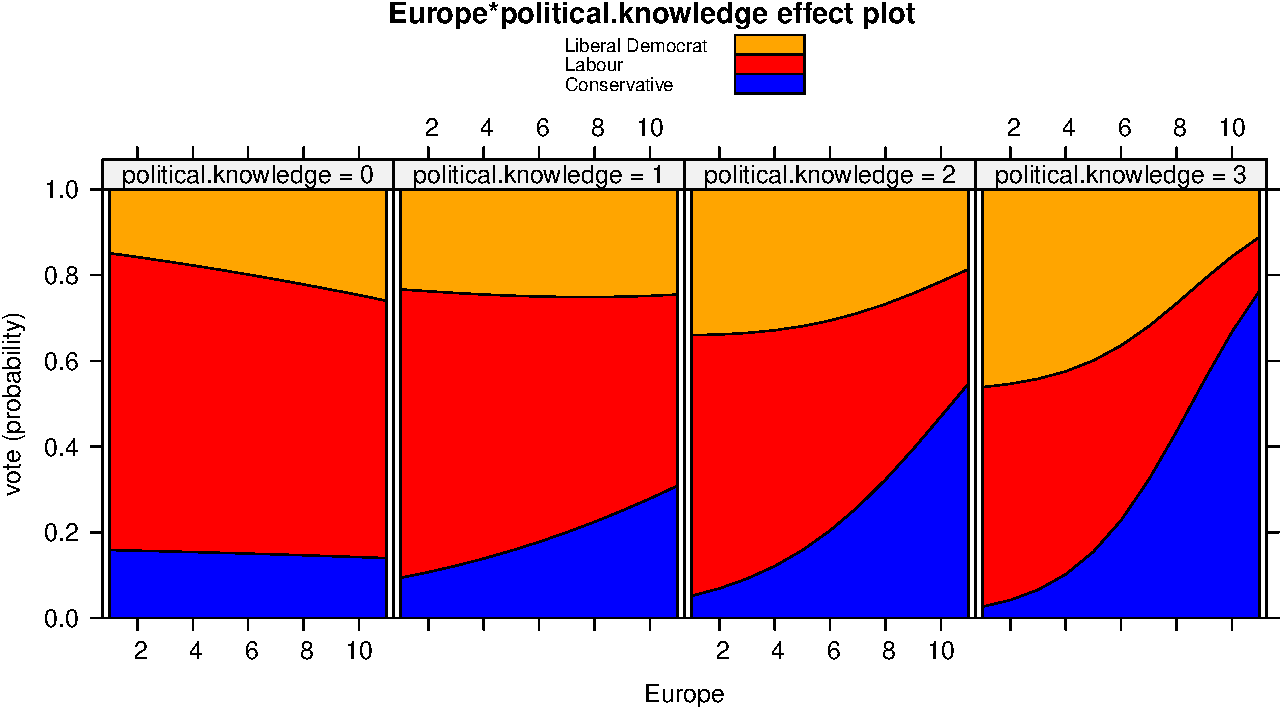
\includegraphics{JSS-article_files/figure-latex/BEPS-plot-1} \end{center}

\end{CodeChunk}

To cross-validate this multinomial-logit model we need an appropriate
cost criterion. None of the criteria supplied by the \textbf{cv}
package---for example, neither \texttt{mse()}, which is appropriate for
a numeric response, nor \texttt{BayesRule()}, which is appropriate for a
binary response---will do. One possibility is to adapt Bayes rule to a
polytomous response:

\begin{CodeChunk}
\begin{CodeInput}
R> head(BEPS$vote)
\end{CodeInput}
\begin{CodeOutput}
[1] Liberal Democrat Labour           Labour           Labour          
[5] Labour           Labour          
Levels: Conservative Labour Liberal Democrat
\end{CodeOutput}
\begin{CodeInput}
R> yhat <- predict(m.beps, type="class")
R> head(yhat)
\end{CodeInput}
\begin{CodeOutput}
[1] Labour           Labour           Labour           Labour          
[5] Liberal Democrat Labour          
Levels: Conservative Labour Liberal Democrat
\end{CodeOutput}
\begin{CodeInput}
R> BayesRuleMulti <- function(y, yhat){
+   result <- mean(y != yhat)
+   attr(result, "casewise loss") <- "y != yhat"
+   result
+ }
R> 
R> BayesRuleMulti(BEPS$vote, yhat)
\end{CodeInput}
\begin{CodeOutput}
[1] 0.3186885
attr(,"casewise loss")
[1] "y != yhat"
\end{CodeOutput}
\end{CodeChunk}

The \texttt{predict()} method for \texttt{"multinom"} models called with
argument \texttt{type="class"} reports the Bayes-rule prediction for
each case---that is, the response category with the highest predicted
probability. Our \texttt{BayesRuleMulti()} function calculates the
proportion of misclassified cases. Because this value is the mean of
casewise components, we attach a \texttt{"casewise\ loss"} attribute to
the result (as explained in the preceding section).

The marginal proportions for the response categories are

\begin{CodeChunk}
\begin{CodeInput}
R> xtabs(~ vote, data=BEPS)/nrow(BEPS)
\end{CodeInput}
\begin{CodeOutput}
vote
    Conservative           Labour Liberal Democrat 
       0.3029508        0.4721311        0.2249180 
\end{CodeOutput}
\end{CodeChunk}

and so the marginal Bayes-rule prediction, that everyone will vote
Labour, produces an error rate of \(1 - 0.47213 = 0.52787\). The
multinomial-logit model appears to do substantially better than that,
but does its performance hold up to cross-validation?

We check first whether the default \texttt{cv()} method works
``out-of-the-box'' for the \texttt{"multinom"} model:

\begin{CodeChunk}
\begin{CodeInput}
R> cv(m.beps, seed=3465, criterion=BayesRuleMulti)
\end{CodeInput}
\begin{CodeOutput}
Error in GetResponse.default(model): non-vector response
\end{CodeOutput}
\end{CodeChunk}

The default method of \texttt{GetResponse()} (a function supplied by the
\textbf{cv} package---see \texttt{?GetResponse}) fails for a
\texttt{"multinom"} object. A straightforward solution is to supply a
\texttt{GetResponse.multinom()} method that returns the factor response
\citep[using the \texttt{get\_response()} function from the
\textbf{insight} package,][]{LudeckeWaggonerMakowski:2019},

\begin{CodeChunk}
\begin{CodeInput}
R> GetResponse.multinom <- function(model, ...) {
+   insight::get_response(model)
+ }
R> 
R> head(GetResponse(m.beps))
\end{CodeInput}
\begin{CodeOutput}
[1] Liberal Democrat Labour           Labour           Labour          
[5] Labour           Labour          
Levels: Conservative Labour Liberal Democrat
\end{CodeOutput}
\end{CodeChunk}

and to try again:

\begin{CodeChunk}
\begin{CodeInput}
R> cv(m.beps, seed=3465, criterion=BayesRuleMulti)
\end{CodeInput}
\begin{CodeOutput}
R RNG seed set to 3465
\end{CodeOutput}
\begin{CodeOutput}
# weights:  36 (22 variable)
initial  value 1507.296060 
iter  10 value 1134.575036
iter  20 value 1037.413231
iter  30 value 1007.705242
iter  30 value 1007.705235
iter  30 value 1007.705235
final  value 1007.705235 
converged
\end{CodeOutput}
\begin{CodeOutput}
Error in match.arg(type): 'arg' should be one of "class", "probs"
\end{CodeOutput}
\end{CodeChunk}

A \texttt{traceback()} (not shown) reveals that the problem is that the
default method of \texttt{cv()} calls the \texttt{"multinom"} method for
\texttt{predict()} with the argument \texttt{type="response"}, when the
correct argument should be \texttt{type="class"}. We therefore must
write a ``\texttt{multinom}'' method for \texttt{cv()}, but that proves
to be very simple:

\begin{CodeChunk}
\begin{CodeInput}
R> cv.multinom <- function (model, data, criterion=BayesRuleMulti, k, reps,
+                          seed, ...){
+   NextMethod(type="class", criterion=criterion)
+ }
\end{CodeInput}
\end{CodeChunk}

That is, we simply call the default \texttt{cv()} method with the
\texttt{type} argument properly set. In addition to supplying the
correct \texttt{type} argument, our method sets the default
\texttt{criterion} for the \texttt{cv.multinom()} method to
\texttt{BayesRuleMulti}.

Then:

\begin{CodeChunk}
\begin{CodeInput}
R> m.beps <- update(m.beps, trace=FALSE)
R> cv(m.beps, seed=3465)
\end{CodeInput}
\begin{CodeOutput}
R RNG seed set to 3465
\end{CodeOutput}
\begin{CodeOutput}
10-Fold Cross Validation
cross-validation criterion = 0.3245902
bias-adjusted cross-validation criterion = 0.3236756
95% CI for bias-adjusted CV criterion = (0.300168, 0.3471831)
full-sample criterion = 0.3186885 
\end{CodeOutput}
\end{CodeChunk}

Prior to invoking \texttt{cv()}, we called \texttt{update()} with
\texttt{trace=FALSE} to suppress the iteration history reported by
default by \texttt{multinom()}---it would be tedious to see the
iteration history for each fold. The cross-validated polytomous
Bayes-rule criterion confirms that the fitted model does substantially
better than the marginal Bayes-rule prediction that everyone votes for
Labour.

\hypertarget{mixed-effects-models}{%
\subsubsection{Mixed-effects models}\label{mixed-effects-models}}

Adding a \texttt{cv()} method for a mixed-model class is somewhat more
complicated. We provide the \texttt{cvMixed()} function to facilitate
this process, and to see how that works, consider the \texttt{"lme"}
method from the \textbf{cv} package:

\begin{CodeChunk}
\begin{CodeInput}
R> cv:::cv.lme
\end{CodeInput}
\begin{CodeOutput}
function(model, data = insight::get_data(model), criterion = mse,
                   k, reps = 1, seed, ncores = 1, clusterVariables, ...){
  cvMixed(
    model,
    package="nlme",
    data=data,
    criterion=criterion,
    k=k,
    reps=reps,
    seed=seed,
    ncores=ncores,
    clusterVariables=clusterVariables,
    predict.clusters.args=list(object=model,
                               newdata=data,
                               level=0),
    predict.cases.args=list(object=model,
                            newdata=data,
                            level=1),
    ...)
}
<bytecode: 0x117501408>
<environment: namespace:cv>
\end{CodeOutput}
\end{CodeChunk}

Notice that \texttt{cv.lme()} sets up a call to \texttt{cvMixed()},
which does the computational work.

Most of the arguments of \texttt{cvMixed()} are familiar:

\begin{itemize}
\item
  \texttt{model} is the mixed-model object, here of class
  \texttt{"lme"}.
\item
  \texttt{package} is the name of the package in which the
  mixed-modeling function used to fit the model, here \texttt{lme()},
  resides---i.e., \texttt{"nlme"}; \texttt{cvMixed()} uses this argument
  to retrieve the package namespace.
\item
  \texttt{data} is the data set to which the model is fit, by default
  extracted by the \texttt{get\_data()} function in the \textbf{insight}
  package.
\item
  \texttt{criterion} is the CV criterion, defaulting to the
  \texttt{mse()} function.
\item
  \texttt{k} is the number of CV folds, defaulting to \texttt{"loo"} for
  CV by clusters and \texttt{10} for CV by cases.
\item
  \texttt{reps} is the number of times the CV process is repeated,
  defaulting to \texttt{1}.
\item
  \texttt{seed} is the seed for R's random-number generator, defaulting
  to a randomly selected (and saved) value.
\item
  \texttt{ncores} is the number of cores to use for parallel
  computation; if \texttt{1}, the default, then the computation isn't
  parallelized.
\item
  \texttt{clusterVariables} is a character vector of the names of
  variables defining clusters; if missing, then CV is based on cases
  rather than clusters.
\end{itemize}

The remaining two arguments are unfamiliar:

\begin{itemize}
\item
  \texttt{predict.clusters.args} is a named list of arguments to be
  passed to the \texttt{predict()} function to obtain predictions for
  the full data set from a model fit to a subset of the data for
  cluster-based CV. The first two arguments should be \texttt{object}
  and \texttt{newdata}. It is typically necessary to tell
  \texttt{cvMixed()} how to base predictions only on fixed effects; in
  the case of \texttt{"lme"} models, this is done by setting
  \texttt{level\ =\ 0}.
\item
  Similarly, \texttt{predict.cases.args} is a named list of arguments to
  be passed to \texttt{predict()} for case-based CV. Setting
  \texttt{level\ =\ 1} includes random effects in the predictions.
\end{itemize}

Finally, any additional arguments, absorbed by \texttt{...}, are passed
to \texttt{update()} when the model is refit with each fold omitted.
\texttt{cvMixed()} returns an object of class \texttt{"cv"}.

Now imagine that we want to support a new class of mixed-effects models.
To be concrete, we illustrate with the \texttt{glmmPQL()} function in
the \textbf{MASS} package \citep{VenablesRipley:2002}, which fits
generalized-linear mixed-effects models by penalized
quasi-likelihood.\footnote{This example is somewhat artificial in that
  \texttt{glmmPQL()} has largely been superseded by computationally
  superior functions, such the \texttt{glmer()} function in the
  \textbf{lme4} package. There is, however, one situation in which
  \texttt{glmmPQL()} might prove useful: to specify serial dependency in
  case-level errors within clusters for longitudinal data, which is not
  currently supported by \texttt{glmer()}.} Not coincidentally, the
arguments of \texttt{glmmPQL()} are similar to those of \texttt{lme()}
(with an additional \texttt{family} argument), because the former
iteratively invokes the latter; so \texttt{cv.glmmPQL()} should resemble
\texttt{cv.lme()}.

As it turns out, neither the default method for \texttt{GetResponse()}
nor \texttt{insight::get\_data()} work for \texttt{"glmmPQL"} objects.
These objects include a \texttt{"data"} element, however, and so we can
simply extract this element as the default for the \texttt{data}
argument of our \texttt{cv.glmmPQL()} method.

To get the response variable is more complicated: We refit the fixed
part of the model as a GLM with only the regression constant on the
right-hand side, and extract the response from that; because all we need
is the response variable, we limit the number of GLM iterations to 1 and
suppress warning messages about non-convergence:

\begin{CodeChunk}
\begin{CodeInput}
R> GetResponse.glmmPQL <- function(model, ...){
+   f <- formula(model)
+   f[[3]] <- 1 # regression constant only on RHS
+   model <- suppressWarnings(glm(f, data=model$data, family=model$family,
+                                 control=list(maxit=1)))
+   cv::GetResponse(model)
+ }
\end{CodeInput}
\end{CodeChunk}

Writing the \texttt{cv()} method is then straightforward:

\begin{CodeChunk}
\begin{CodeInput}
R> cv.glmmPQL <- function(model, data = model$data, criterion = mse,
+                      k, reps = 1, seed, ncores = 1, clusterVariables, ...){
+   cvMixed(
+     model,
+     package="MASS",
+     data=data,
+     criterion=criterion,
+     k=k,
+     reps=reps,
+     seed=seed,
+     ncores=ncores,
+     clusterVariables=clusterVariables,
+     predict.clusters.args=list(object=model,
+                                newdata=data,
+                                level=0,
+                                type="response"),
+     predict.cases.args=list(object=model,
+                             newdata=data,
+                             level=1,
+                             type="response"),
+     verbose=FALSE,
+     ...)
+ }
\end{CodeInput}
\end{CodeChunk}

We set the argument \texttt{verbose=FALSE} to suppress
\texttt{glmmPQL()}'s iteration counter when \texttt{cvMixed()} calls
\texttt{update()}.

Let's apply our newly minted method to a logistic regression with a
random intercept in an example that appears in \texttt{?glmmPQL}:

\begin{CodeChunk}
\begin{CodeInput}
R> library("MASS")
R> m.pql <- glmmPQL(y ~ trt + I(week > 2), random = ~ 1 | ID,
+              family = binomial, data = bacteria)
\end{CodeInput}
\begin{CodeOutput}
iteration 1
\end{CodeOutput}
\begin{CodeOutput}
iteration 2
\end{CodeOutput}
\begin{CodeOutput}
iteration 3
\end{CodeOutput}
\begin{CodeOutput}
iteration 4
\end{CodeOutput}
\begin{CodeOutput}
iteration 5
\end{CodeOutput}
\begin{CodeOutput}
iteration 6
\end{CodeOutput}
\begin{CodeInput}
R> summary(m.pql)
\end{CodeInput}
\begin{CodeOutput}
Linear mixed-effects model fit by maximum likelihood
  Data: bacteria 
  AIC BIC logLik
   NA  NA     NA

Random effects:
 Formula: ~1 | ID
        (Intercept)  Residual
StdDev:    1.410637 0.7800511

Variance function:
 Structure: fixed weights
 Formula: ~invwt 
Fixed effects:  y ~ trt + I(week > 2) 
                    Value Std.Error  DF   t-value p-value
(Intercept)      3.412014 0.5185033 169  6.580506  0.0000
trtdrug         -1.247355 0.6440635  47 -1.936696  0.0588
trtdrug+        -0.754327 0.6453978  47 -1.168779  0.2484
I(week > 2)TRUE -1.607257 0.3583379 169 -4.485311  0.0000
 Correlation: 
                (Intr) trtdrg trtdr+
trtdrug         -0.598              
trtdrug+        -0.571  0.460       
I(week > 2)TRUE -0.537  0.047 -0.001

Standardized Within-Group Residuals:
       Min         Q1        Med         Q3        Max 
-5.1985361  0.1572336  0.3513075  0.4949482  1.7448845 

Number of Observations: 220
Number of Groups: 50 
\end{CodeOutput}
\end{CodeChunk}

We compare this result to that obtained from \texttt{glmer()} in the
\textbf{lme4} package:

\begin{CodeChunk}
\begin{CodeInput}
R> library("lme4")
R> m.glmer <- glmer(y ~ trt + I(week > 2) + (1 | ID),
+                family = binomial, data = bacteria)
R> summary(m.glmer)
\end{CodeInput}
\begin{CodeOutput}
Generalized linear mixed model fit by maximum likelihood (Laplace
  Approximation) [glmerMod]
 Family: binomial  ( logit )
Formula: y ~ trt + I(week > 2) + (1 | ID)
   Data: bacteria

     AIC      BIC   logLik deviance df.resid 
   202.3    219.2    -96.1    192.3      215 

Scaled residuals: 
    Min      1Q  Median      3Q     Max 
-4.5615  0.1359  0.3022  0.4217  1.1276 

Random effects:
 Groups Name        Variance Std.Dev.
 ID     (Intercept) 1.543    1.242   
Number of obs: 220, groups:  ID, 50

Fixed effects:
                Estimate Std. Error z value Pr(>|z|)
(Intercept)       3.5479     0.6958   5.099 3.41e-07
trtdrug          -1.3667     0.6770  -2.019 0.043517
trtdrug+         -0.7826     0.6831  -1.146 0.251925
I(week > 2)TRUE  -1.5985     0.4759  -3.359 0.000783

Correlation of Fixed Effects:
            (Intr) trtdrg trtdr+
trtdrug     -0.593              
trtdrug+    -0.537  0.487       
I(wk>2)TRUE -0.656  0.126  0.064
\end{CodeOutput}
\begin{CodeInput}
R>   # comparison of fixed effects:
R> car::compareCoefs(m.pql, m.glmer) 
\end{CodeInput}
\begin{CodeOutput}
Warning in car::compareCoefs(m.pql, m.glmer): models to be compared are of
different classes
\end{CodeOutput}
\begin{CodeOutput}
Calls:
1: glmmPQL(fixed = y ~ trt + I(week > 2), random = ~1 | ID, family = 
  binomial, data = bacteria)
2: glmer(formula = y ~ trt + I(week > 2) + (1 | ID), data = bacteria, 
  family = binomial)

                Model 1 Model 2
(Intercept)       3.412   3.548
SE                0.514   0.696
                               
trtdrug          -1.247  -1.367
SE                0.638   0.677
                               
trtdrug+         -0.754  -0.783
SE                0.640   0.683
                               
I(week > 2)TRUE  -1.607  -1.598
SE                0.355   0.476
                               
\end{CodeOutput}
\end{CodeChunk}

The two sets of estimates are similar, but not identical

Finally, we try out our \texttt{cv.glmmPQL()} method, cross-validating
both by clusters and by cases,

\begin{CodeChunk}
\begin{CodeInput}
R> cv(m.pql, clusterVariables="ID", criterion=BayesRule)
\end{CodeInput}
\begin{CodeOutput}
n-Fold Cross Validation based on 50 {ID} clusters
cross-validation criterion = 0.1954545
bias-adjusted cross-validation criterion = 0.1954545
full-sample criterion = 0.1954545 
\end{CodeOutput}
\begin{CodeInput}
R> cv(m.pql, data=bacteria, criterion=BayesRule, seed=1490)
\end{CodeInput}
\begin{CodeOutput}
R RNG seed set to 1490
\end{CodeOutput}
\begin{CodeOutput}
10-Fold Cross Validation
cross-validation criterion = 0.2090909
bias-adjusted cross-validation criterion = 0.2072727
full-sample criterion = 0.1454545 
\end{CodeOutput}
\end{CodeChunk}

and again compare to \texttt{glmer()}:

\begin{CodeChunk}
\begin{CodeInput}
R> cv(m.glmer, clusterVariables="ID", criterion=BayesRule)
\end{CodeInput}
\begin{CodeOutput}
n-Fold Cross Validation based on 50 {ID} clusters
cross-validation criterion = 0.1954545
bias-adjusted cross-validation criterion = 0.1954545
full-sample criterion = 0.1954545 
\end{CodeOutput}
\begin{CodeInput}
R> cv(m.glmer, data=bacteria, criterion=BayesRule, seed=1490)
\end{CodeInput}
\begin{CodeOutput}
R RNG seed set to 1490
\end{CodeOutput}
\begin{CodeOutput}
10-Fold Cross Validation
cross-validation criterion = 0.1954545
bias-adjusted cross-validation criterion = 0.1936364
full-sample criterion = 0.15 
\end{CodeOutput}
\end{CodeChunk}

\hypertarget{adding-a-model-selection-procedure}{%
\subsection{Adding a model-selection
procedure}\label{adding-a-model-selection-procedure}}

The \texttt{selectStepAIC()} function supplied by the \textbf{cv}
package, which is based on the \texttt{stepAIC()} function from the
\textbf{nnet} package \citep{VenablesRipley:2002} for stepwise model
selection, is suitable for the \texttt{procedure} argument of
\texttt{cvSelect()}. The use of \texttt{selectStepAIC()} is illustrated
in the principal vignette for the package.

We'll employ \texttt{selectStepAIC()} as a ``template'' for writing a CV
model-selection procedure. To see the code for this function, type
\texttt{cv::selectStepAIC} at the R command prompt, or examine the
sources for the \textbf{cv} package at
\url{https://github.com/gmonette/cv} (the code for
\texttt{selectStepAIC()} is in
\url{https://github.com/gmonette/cv/blob/main/R/cvSelect.R}).

Another approach to model selection is all-subsets regression. The
\texttt{regsubsets()} function in the \textbf{leaps} package
\citep{LumleyMiller:2020} implements an efficient algorithm for
selecting the best-fitting linear least-squares regressions for subsets
of predictors of all sizes, from 1 through the maximum number of
candidate predictors.\footnote{The \texttt{regsubsets()} function
  computes several measures of model predictive performance, including
  the \(R^2\) and \(R^2\) adjusted for degrees of freedom, the residual
  sums of squares, Mallows's \(C_p\), and the BIC. Several of these are
  suitable for comparing models with differing numbers of
  coefficients---we use the BIC below---but all necessarily agree when
  comparing models with the \emph{same} number of coefficients.} To
illustrate the use of \texttt{regsubsets()}, we employ the
\texttt{swiss} data frame supplied by the \textbf{leaps} package:

\begin{CodeChunk}
\begin{CodeInput}
R> library("leaps")
R> head(swiss)
\end{CodeInput}
\begin{CodeOutput}
             Fertility Agriculture Examination Education Catholic
Courtelary        80.2        17.0          15        12     9.96
Delemont          83.1        45.1           6         9    84.84
Franches-Mnt      92.5        39.7           5         5    93.40
Moutier           85.8        36.5          12         7    33.77
Neuveville        76.9        43.5          17        15     5.16
Porrentruy        76.1        35.3           9         7    90.57
             Infant.Mortality
Courtelary               22.2
Delemont                 22.2
Franches-Mnt             20.2
Moutier                  20.3
Neuveville               20.6
Porrentruy               26.6
\end{CodeOutput}
\begin{CodeInput}
R> nrow(swiss)
\end{CodeInput}
\begin{CodeOutput}
[1] 47
\end{CodeOutput}
\end{CodeChunk}

The data set includes the following variables, for each of 47
French-speaking Swiss provinces circa 1888:

\begin{itemize}
\tightlist
\item
  \texttt{Fertility}: A standardized fertility measure.
\item
  \texttt{Agriculture}: The percentage of the male population engaged in
  agriculture.
\item
  \texttt{Examination}: The percentage of draftees into the Swiss army
  receiving the highest grade on an examination.
\item
  \texttt{Education}: The percentage of draftees with more than a
  primary-school education.
\item
  \texttt{Catholic}: The percentage of the population who were Catholic.
\item
  \texttt{Infant.Mortality}: The infant-mortality rate, expressed as the
  percentage of live births surviving less than a year.
\end{itemize}

Following \citet{LumleyMiller:2020}, we treat \texttt{Fertility} as the
response and the other variables as predictors in a linear least-squares
regression:

\begin{CodeChunk}
\begin{CodeInput}
R> m.swiss <- lm(Fertility ~ ., data=swiss)
R> summary(m.swiss)
\end{CodeInput}
\begin{CodeOutput}

Call:
lm(formula = Fertility ~ ., data = swiss)

Residuals:
     Min       1Q   Median       3Q      Max 
-15.2743  -5.2617   0.5032   4.1198  15.3213 

Coefficients:
                 Estimate Std. Error t value Pr(>|t|)
(Intercept)      66.91518   10.70604   6.250 1.91e-07
Agriculture      -0.17211    0.07030  -2.448  0.01873
Examination      -0.25801    0.25388  -1.016  0.31546
Education        -0.87094    0.18303  -4.758 2.43e-05
Catholic          0.10412    0.03526   2.953  0.00519
Infant.Mortality  1.07705    0.38172   2.822  0.00734

Residual standard error: 7.165 on 41 degrees of freedom
Multiple R-squared:  0.7067,    Adjusted R-squared:  0.671 
F-statistic: 19.76 on 5 and 41 DF,  p-value: 5.594e-10
\end{CodeOutput}
\begin{CodeInput}
R> cv(m.swiss, seed=8433)
\end{CodeInput}
\begin{CodeOutput}
R RNG seed set to 8433
\end{CodeOutput}
\begin{CodeOutput}
10-Fold Cross Validation
method: Woodbury
criterion: mse
cross-validation criterion = 59.68315
bias-adjusted cross-validation criterion = 58.84614
full-sample criterion = 44.78815 
\end{CodeOutput}
\end{CodeChunk}

Thus, the RMSE for the model fit to the complete data is considerably
smaller than the CV estimate of the RMSE. Can we do better by selecting
a subset of the predictors, taking account of the additional uncertainty
induced by model selection?

First, let's apply best-subset selection to the complete data set:

\begin{CodeChunk}
\begin{CodeInput}
R> swiss.sub <- regsubsets(Fertility ~ ., data=swiss)
R> summary(swiss.sub)
\end{CodeInput}
\begin{CodeOutput}
Subset selection object
Call: regsubsets.formula(Fertility ~ ., data = swiss)
5 Variables  (and intercept)
                 Forced in Forced out
Agriculture          FALSE      FALSE
Examination          FALSE      FALSE
Education            FALSE      FALSE
Catholic             FALSE      FALSE
Infant.Mortality     FALSE      FALSE
1 subsets of each size up to 5
Selection Algorithm: exhaustive
         Agriculture Examination Education Catholic Infant.Mortality
1  ( 1 ) " "         " "         "*"       " "      " "             
2  ( 1 ) " "         " "         "*"       "*"      " "             
3  ( 1 ) " "         " "         "*"       "*"      "*"             
4  ( 1 ) "*"         " "         "*"       "*"      "*"             
5  ( 1 ) "*"         "*"         "*"       "*"      "*"             
\end{CodeOutput}
\begin{CodeInput}
R> (bics <- summary(swiss.sub)$bic)
\end{CodeInput}
\begin{CodeOutput}
[1] -19.60287 -28.61139 -35.65643 -37.23388 -34.55301
\end{CodeOutput}
\begin{CodeInput}
R> which.min(bics)
\end{CodeInput}
\begin{CodeOutput}
[1] 4
\end{CodeOutput}
\begin{CodeInput}
R> car::subsets(swiss.sub, legend="topright")
\end{CodeInput}
\begin{figure}

{\centering 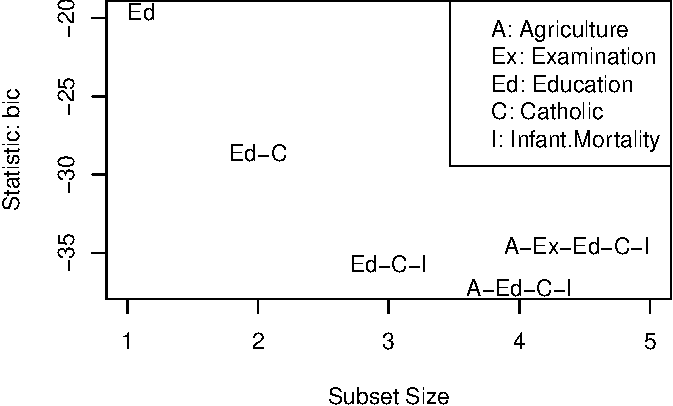
\includegraphics{JSS-article_files/figure-latex/subset-selection-1} 

}

\caption[Selecting the best model of each size]{Selecting the best model of each size.}\label{fig:subset-selection}
\end{figure}
\end{CodeChunk}

The graph, produced by the \texttt{subsets()} function in the
\textbf{car} package, shows that the model with the smallest BIC is the
best model with 4 predictors, including \texttt{Agriculture},
\texttt{Education}, \texttt{Catholic}, and \texttt{Infant.Mortality},
but not \texttt{Examination}:

\begin{CodeChunk}
\begin{CodeInput}
R> m.best <- update(m.swiss, . ~ . - Examination)
R> summary(m.best)
\end{CodeInput}
\begin{CodeOutput}

Call:
lm(formula = Fertility ~ Agriculture + Education + Catholic + 
    Infant.Mortality, data = swiss)

Residuals:
     Min       1Q   Median       3Q      Max 
-14.6765  -6.0522   0.7514   3.1664  16.1422 

Coefficients:
                 Estimate Std. Error t value Pr(>|t|)
(Intercept)      62.10131    9.60489   6.466 8.49e-08
Agriculture      -0.15462    0.06819  -2.267  0.02857
Education        -0.98026    0.14814  -6.617 5.14e-08
Catholic          0.12467    0.02889   4.315 9.50e-05
Infant.Mortality  1.07844    0.38187   2.824  0.00722

Residual standard error: 7.168 on 42 degrees of freedom
Multiple R-squared:  0.6993,    Adjusted R-squared:  0.6707 
F-statistic: 24.42 on 4 and 42 DF,  p-value: 1.717e-10
\end{CodeOutput}
\begin{CodeInput}
R> cv(m.best, seed=8433) # use same folds as before
\end{CodeInput}
\begin{CodeOutput}
R RNG seed set to 8433
\end{CodeOutput}
\begin{CodeOutput}
10-Fold Cross Validation
method: Woodbury
criterion: mse
cross-validation criterion = 58.46664
bias-adjusted cross-validation criterion = 57.7779
full-sample criterion = 45.91637 
\end{CodeOutput}
\end{CodeChunk}

The RMSE for the selected model is (of course) slightly higher than for
the full model fit previously, but the cross-validated RMSE is a bit
lower; as we explain in the main vignette, however, it isn't kosher to
select and cross-validate a model on the same data.

Here's a function named \texttt{selectSubsets()}, meant to be used with
\texttt{cvSelect()}, suitable for cross-validating the model-selection
process:

\begin{CodeChunk}
\begin{CodeInput}
R> selectSubsets <- function(data=insight::get_data(model), 
+                           model,
+                           indices,
+                           criterion=mse,
+                           save.coef=TRUE, ...){
+   
+   if (inherits(model, "lm", which=TRUE) != 1)
+     stop("selectSubsets is appropriate only for 'lm' models")
+   
+   y <- GetResponse(model)
+   formula <- formula(model)
+   X <- model.matrix(model)
+ 
+   if (missing(indices)) {
+     # select the best model from the full data by BIC
+     sel <- leaps::regsubsets(formula, data=data, ...)
+     bics <- summary(sel)$bic
+     best <- coef(sel, 1:length(bics))[[which.min(bics)]]
+     x.names <- names(best)
+     # fit the best model; intercept is already in X, hence - 1:
+     m.best <- lm(y ~ X[, x.names] - 1) 
+     fit.all <- predict(m.best, newdata=data)
+     return(criterion(y, fit.all)) # return the CV criterion
+   }
+ 
+   # select the best model omitting the i-th fold (given by indices)
+   sel.i <- leaps::regsubsets(formula, data[-indices, ], ...)
+   bics.i <- summary(sel.i)$bic
+   best.i <- coef(sel.i, 1:length(bics.i))[[which.min(bics.i)]]
+   x.names.i <- names(best.i)
+   m.best.i <- lm(y[-indices] ~ X[-indices, x.names.i] - 1)
+               # predict() doesn't work here:
+   fit.all.i <- as.vector(X[, x.names.i] %*% coef(m.best.i))
+   fit.i <- fit.all.i[indices]
+   # return the fitted values for i-th fold, CV criterion for all cases, 
+   #   and the regression coefficients
+   list(fit.i=fit.i, # fitted values for i-th fold
+        crit.all.i=criterion(y, fit.all.i), # CV crit for all cases
+        coefficients = if (save.coef){ # regression coefficients
+          coefs <- coef(m.best.i)
+          
+          # fix coefficient names
+          names(coefs) <- sub("X\\[-indices, x.names.i\\]", "",
+                              names(coefs))
+          
+          coefs
+        }  else {
+          NULL
+        }
+   )
+ }
\end{CodeInput}
\end{CodeChunk}

A slightly tricky point is that because of scoping issues,
\texttt{predict()} doesn't work with the model fit omitting the \(i\)th
fold, and so the fitted values for all cases are computed directly as
\(\widehat{\mathbf{y}}_{-i} = \mathbf{X} \mathbf{b}_{-i}\), where
\(\mathbf{X}\) is the model-matrix for all of the cases, and
\(\mathbf{b}_{-i}\) is the vector of least-squares coefficients for the
selected model with the \(i\)th fold omitted.

Additionally, the command
\texttt{lm(y{[}-indices{]}\ \textasciitilde{}\ X{[}-indices,\ x.names.i{]}\ -\ 1)},
which is the selected model with the \(i\)th fold deleted, produces
awkward coefficient names like
\texttt{"X{[}-indices,\ x.names.i{]}Infant.Mortality"}. Purely for
aesthetic reasons, the command
\texttt{sub("X\textbackslash{}\textbackslash{}{[}-indices,\ x.names.i\textbackslash{}\textbackslash{}{]}",\ "",\ names(coefs))}
fixes these awkward names, removing the extraneous text,
\texttt{"X{[}-indices,\ x.names.i{]}"}.

Applying \texttt{selectSubsets()} to the full data produces the
full-data cross-validated RMSE (which we obtained previously):
\%\%\texttt{\{r\ test-selectSubsets\}\ \%\%selectSubsets(model=m.swiss)\ \%\%}
Similarly, applying the function to an imaginary ``fold'' of 5 cases
returns the RMSE for the cases in the fold, based on the model selected
and fit to the cases omitting the fold; the RMSE for all of the cases,
based on the same model; and the coefficients of the selected model,
which includes 4 or the 5 predictors (and the intercept):
\%\%\texttt{\{r\ test-selectSubsets-fold\}\ \%\%selectSubsets(model=m.swiss,\ indices=seq(5,\ 45,\ by=10))\ \%\%}

Then, using \texttt{selectSubsets()} in cross-validation, we get:

\begin{CodeChunk}
\begin{CodeInput}
R> (cv.swiss <- cvSelect(selectSubsets, model=m.swiss,
+                       data=swiss, seed=8433)) # use same folds
\end{CodeInput}
\begin{CodeOutput}
R RNG seed set to 8433
\end{CodeOutput}
\begin{CodeOutput}
10-Fold Cross Validation
cross-validation criterion = 65.83495
bias-adjusted cross-validation criterion = 63.64431
full-sample criterion = 45.91637 
\end{CodeOutput}
\end{CodeChunk}

Cross-validation shows that model selection exacts a penalty in RMSE.
Examining the models selected for the 10 folds reveals that there is
some uncertainty in identifying the predictors in the ``best'' model,
with \texttt{Agriculture} sometimes appearing and sometimes not:

\begin{CodeChunk}
\begin{CodeInput}
R> compareFolds(cv.swiss)
\end{CodeInput}
\begin{CodeOutput}
        (Intercept) Catholic Education Infant.Mortality Agriculture
Fold 1      59.0852   0.1397   -1.0203           1.2985       -0.17
Fold 2      67.0335   0.1367   -1.0499           0.9413       -0.20
Fold 3      55.0453   0.1221   -0.8757           1.3541       -0.15
Fold 4      62.5543   0.1236   -0.9719           1.0679       -0.16
Fold 5      50.4643   0.1057   -0.7863           1.2144            
Fold 6      68.0289   0.1195   -1.0073           0.8294       -0.17
Fold 7      66.5219   0.1357   -1.0827           0.9523       -0.19
Fold 8      46.3507   0.0776   -0.7637           1.4463            
Fold 9      62.2632   0.1230   -1.0067           1.1000       -0.17
Fold 10     52.5112   0.1005   -0.7232           1.0809            
\end{CodeOutput}
\end{CodeChunk}

\hypertarget{computational-notes}{%
\section{Computational notes}\label{computational-notes}}

\hypertarget{efficient-computations-for-linear-and-generalized-linear-models}{%
\subsection{Efficient computations for linear and generalized linear
models}\label{efficient-computations-for-linear-and-generalized-linear-models}}

The most straightforward way to implement cross-validation in R for
statistical modeling functions that are written in the canonical manner
is to use \texttt{update()} to refit the model with each fold removed.
This is the approach taken in the default method for \texttt{cv()}, and
it is appropriate if the cases are independently sampled. Refitting the
model in this manner for each fold is generally feasible when the number
of folds in modest, but can be prohibitively costly for leave-one-out
cross-validation when the number of cases is large.

The \texttt{"lm"} and \texttt{"glm"} methods for \texttt{cv()} take
advantage of computational efficiencies by avoiding refitting the model
with each fold removed. Consider, in particular, the weighted linear
model
\(\mathbf{y}_{n \times 1} = \mathbf{X}_{n \times p}\boldsymbol{\beta}_{p \times 1} + \boldsymbol{\varepsilon}_{n \times 1}\),
where
\(\boldsymbol{\varepsilon} \sim \mathbf{N}_n \left(\mathbf{0}, \sigma^2 \mathbf{W}^{-1}_{n \times n}\right)\).
Here, \(\mathbf{y}\) is the response vector, \(\mathbf{X}\) the model
matrix, and \(\boldsymbol{\varepsilon}\) the error vector, each for
\(n\) cases, and \(\boldsymbol{\beta}\) is the vector of \(p\)
population regression coefficients. The errors are assumed to be
multivariately normally distributed with 0 means and covariance matrix
\(\sigma^2 \mathbf{W}^{-1}\), where \(\mathbf{W} = \mathrm{diag}(w_i)\)
is a diagonal matrix of inverse-variance weights. For the linear model
with constant error variance, the weight matrix is taken to be
\(\mathbf{W} = \mathbf{I}_n\), the order-\(n\) identity matrix.

The weighted-least-squares (WLS) estimator of \(\boldsymbol{\beta}\) is
\citep[see, e.g.,][Sec. 12.2.2]{Fox:2016} \footnote{This is a
  definitional formula, which assumes that the model matrix
  \(\mathbf{X}\) is of full column rank, and which can be subject to
  numerical instability when \(\mathbf{X}\) is ill-conditioned.
  \texttt{lm()} uses the singular-value decomposition of the model
  matrix to obtain computationally more stable results.} \[
\mathbf{b}_{\mathrm{WLS}} = \left( \mathbf{X}^T \mathbf{W} \mathbf{X} \right)^{-1} 
  \mathbf{X}^T \mathbf{W} \mathbf{y}
\]

Fitted values are then
\(\widehat{\mathbf{y}} = \mathbf{X}\mathbf{b}_{\mathrm{WLS}}\).

The LOO fitted value for the \(i\)th case can be efficiently computed by
\(\widehat{y}_{-i} = y_i - e_i/(1 - h_i)\) where
\(h_i = \mathbf{x}^T_i \left( \mathbf{X}^T \mathbf{W} \mathbf{X} \right)^{-1} \mathbf{x}_i\)
(the so-called ``hatvalue''). Here, \(\mathbf{x}^T_i\) is the \(i\)th
row of \(\mathbf{X}\), and \(\mathbf{x}_i\) is the \(i\)th row written
as a column vector. This approach can break down when one or more
hatvalues are equal to 1, in which case the formula for
\(\widehat{y}_{-i}\) requires division by 0.

To compute cross-validated fitted values when the folds contain more
than one case, we make use of the Woodbury matrix identify
\citep{Wikipedia-Woodbury:2023}, \[
\left(\mathbf{A}_{m \times m} + \mathbf{U}_{m \times k} 
\mathbf{C}_{k \times k} \mathbf{V}_{k \times m} \right)^{-1} = \mathbf{A}^{-1} - \mathbf{A}^{-1}\mathbf{U} \left(\mathbf{C}^{-1} + 
\mathbf{VA}^{-1}\mathbf{U} \right)^{-1} \mathbf{VA}^{-1}
\] where \(\mathbf{A}\) is a nonsingular order-\(n\) matrix. We apply
this result by letting \begin{align*}
    \mathbf{A} &= \mathbf{X}^T \mathbf{W} \mathbf{X} \\
    \mathbf{U} &= \mathbf{X}_\mathbf{j}^T \\
    \mathbf{V} &= - \mathbf{X}_\mathbf{j} \\
    \mathbf{C} &= \mathbf{W}_\mathbf{j} \\
\end{align*} where the subscript
\(\mathbf{j} = (i_{j1}, \ldots, i_{jm})^T\) represents the vector of
indices for the cases in the \(j\)th fold, \(j = 1, \ldots, k\). The
negative sign in \(\mathbf{V} = - \mathbf{X}_\mathbf{j}\) reflects the
\emph{removal}, rather than addition, of the cases in \(\mathbf{j}\).

Applying the Woodbury identity isn't quite as fast as using the
hatvalues, but it is generally much faster than refitting the model. A
disadvantage of the Woodbury identity, however, is that it entails
explicit matrix inversion and thus may be numerically unstable. The
inverse of \(\mathbf{A} = \mathbf{X}^T \mathbf{W} \mathbf{X}\) is
available directly in the \texttt{"lm"} object, but the second term on
the right-hand side of the Woodbury identity requires a matrix inversion
with each fold deleted. (In contrast, the inverse of each
\(\mathbf{C} = \mathbf{W}_\mathbf{j}\) is straightforward because
\(\mathbf{W}\) is diagonal.)

The Woodbury identity also requires that the model matrix be of full
rank. We impose that restriction in our code by removing redundant
regressors from the model matrix for all of the cases, but that doesn't
preclude rank deficiency from surfacing when a fold is removed. Rank
deficiency of \(\mathbf{X}\) doesn't disqualify cross-validation because
all we need are fitted values under the estimated model.

\texttt{glm()} computes the maximum-likelihood estimates for a
generalized linear model by iterated weighted least squares \citep[see,
e.g.,][Sec. 6.12]{FoxWeisberg:2019}. The last iteration is therefore
just a WLS fit of the ``working response'' on the model matrix using
``working weights.'' Both the working weights and the working response
at convergence are available from the information in the object returned
by \texttt{glm()}.

We then treat re-estimation of the model with a case or cases deleted as
a WLS problem, using the hatvalues or the Woodbury matrix identity. The
resulting fitted values for the deleted fold aren't exact---that is,
except for the Gaussian family, the result isn't identical to what we
would obtain by literally refitting the model---but in our (limited)
experience, the approximation is very good, especially for LOO CV, which
is when we would be most tempted to use it. Nevertheless, because these
results are approximate, the default for the \texttt{"glm"}
\texttt{cv()} method is to perform the exact computation, which entails
refitting the model with each fold omitted.

\hypertarget{computation-of-the-bias-corrected-cv-criterion-and-confidence-intervals}{%
\subsection{Computation of the bias-corrected CV criterion and
confidence
intervals}\label{computation-of-the-bias-corrected-cv-criterion-and-confidence-intervals}}

Let \(\mathrm{CV}(\mathbf{y}, \widehat{\mathbf{y}})\) represent a
cross-validation cost criterion, such as mean-squared error, computed
for all of the \(n\) values of the response \(\mathbf{y}\) based on
fitted values \(\widehat{\mathbf{y}}\) from the model fit to all of the
data. We require that \(\mathrm{CV}(\mathbf{y}, \widehat{\mathbf{y}})\)
is the mean of casewise components, that is,
\(\mathrm{CV}(\mathbf{y}, \widehat{\mathbf{y}}) = \frac{1}{n}\sum_{i=1}^n\mathrm{cv}(y_i, \widehat{y}_i)\).\footnote{\citet{ArlotCelisse:2010}
  term the casewise loss, \(\mathrm{cv}(y_i, \widehat{y}_i)\), the
  ``contrast function.''} For example,
\(\mathrm{MSE}(\mathbf{y}, \widehat{\mathbf{y}}) = \frac{1}{n}\sum_{i=1}^n (y_i - \widehat{y}_i)^2\).

We divide the \(n\) cases into \(k\) folds of approximately
\(n_j \approx n/k\) cases each, where \(n = \sum n_j\). As above, let
\(\mathbf{j}\) denote the indices of the cases in the \(j\)th fold.

Now define
\(\mathrm{CV}_j = \mathrm{CV}(\mathbf{y}, \widehat{\mathbf{y}}^{(j)})\).
The superscript \((j)\) on \(\widehat{\mathbf{y}}^{(j)}\) represents
fitted values computed for all of the cases from the model with fold
\(j\) omitted. Let \(\widehat{\mathbf{y}}^{(-i)}\) represent the vector
of fitted values for all \(n\) cases where the fitted value for the
\(i\)th case is computed from the model fit with the fold including the
\(i\)th case omitted (i.e., fold \(j\) for which \(i \in \mathbf{j}\)).

Then the cross-validation criterion is just
\(\mathrm{CV} = \mathrm{CV}(\mathbf{y}, \widehat{\mathbf{y}}^{(-i)})\).
Following \citet[pp.~293--295]{DavisonHinkley:1997}, the bias-adjusted
cross-validation criterion is \[
\mathrm{CV}_{\mathrm{adj}} = \mathrm{CV} + \mathrm{CV}(\mathbf{y}, \widehat{\mathbf{y}}) - \frac{1}{n} \sum_{j=1}^{k} n_j \mathrm{CV}_j
\]

We compute the standard error of CV as \[
\mathrm{SE}(\mathrm{CV}) = \frac{1}{\sqrt n} \sqrt{ \frac{\sum_{i=1}^n \left[ \mathrm{cv}(y_i, \widehat{y}_i^{(-i)} ) - \mathrm{CV} \right]^2 }{n - 1} }
\] that is, as the standard deviation of the casewise components of CV
divided by the square-root of the number of cases.

We then use \(\mathrm{SE}(\mathrm{CV})\) to construct a
\(100 \times (1 - \alpha)\)\% confidence interval around the
\emph{adjusted} CV estimate of error: \[
\left[ \mathrm{CV}_{\mathrm{adj}} - z_{1 - \alpha/2}\mathrm{SE}(\mathrm{CV}), \mathrm{CV}_{\mathrm{adj}} + z_{1 - \alpha/2}\mathrm{SE}(\mathrm{CV})  \right]
\] where \(z_{1 - \alpha/2}\) is the \(1 - \alpha/2\) quantile of the
standard-normal distribution (e.g, \(z \approx 1.96\) for a 95\%
confidence interval, for which \(1 - \alpha/2 = .975\)).

\citet{BatesHastieTibshirani:2023} show that the coverage of this
confidence interval is poor for small samples, and they suggest a much
more computationally intensive procedure, called \emph{nested
cross-validation}, to compute better estimates of error and confidence
intervals with better coverage for small samples. We may implement Bates
et al.'s approach in a later release of the \textbf{cv} package. At
present we use the confidence interval above for sufficiently large
\(n\), which, based on Bates et al.'s results, we take by default to be
\(n \ge 400\).

\hypertarget{why-the-complement-of-auc-isnt-a-casewise-cv-criterion}{%
\section{Why the complement of AUC isn't a casewise CV
criterion}\label{why-the-complement-of-auc-isnt-a-casewise-cv-criterion}}

Consider calculating AUC for folds in which a validation set contains
\(n_v\) observations. To calculate AUC in the validation set, we need
the vector of prediction criteria,
\(\widehat{\mathbf{y}}_{v_{(n_v \times 1)}} = (\widehat{y}_1, ..., \widehat{y}_{n_v})^T\),
and the vector of observed responses in the validation set,
\(\mathbf{y}_{v_{(n_v \times 1)}} = (y_1, \ldots, y_{n_v})^T\) with
\(y_i \in \{0,1\}, \; i = 1, \ldots, n_v\).

To construct the ROC curve, only the ordering of the values in
\(\mathbf{\widehat{y}}_v\) is relevant. Thus, assuming that there are no
ties, and reordering observations if necessary, we can set
\(\mathbf{\widehat{y}}_v = (1, 2, \ldots, n_v)^T\).

If the AUC can be expressed as the casewise mean or sum of a function
\(\mathrm{cv}(\widehat{y}_i,y_i)\), where
\(\mathrm{cv}: \{1,2,...,n_v\}\times\{0,1\} \rightarrow [0,1]\), then
\begin{equation}
\label{eq:cw}
\tag{1}
\sum_{i=1}^{n_v} \mathrm{cv}(\widehat{y}_i,y_i) = \mathrm{AUC}(\mathbf{\widehat{y}}_v,\mathbf{y}_v)
\end{equation} must hold for all \(2^{n_v}\) possible values of
\(\mathbf{y}_v = (y_1,...,y_{n_v})^T\). If all \(y\mathrm{s}\) have the
same value, either 1 or 0, then the definition of AUC is ambiguous. AUC
could be considered undefined, or it could be set to 0 if all \(y\)s are
0 and to 1 if all \(y\)s are 1. If AUC is considered to be undefined in
these cases, we have \(2^{n_v} - 2\) admissible values for
\(\mathbf{y}_v\).

Thus, equation (\ref{eq:cw}) produces either \(2^{n_v}\) or
\(2^{n_v}-2\) constraints. Although there are only \(2n_v\) possible
values for the \(\mathrm{cv(\cdot)}\) function, equation (\ref{eq:cw})
could, nevertheless, have consistent solutions. We therefore need to
determine whether there is a value of \(n_v\) for which (\ref{eq:cw})
has no consistent solution for all admissible values of
\(\mathbf{y}_v\). In that eventuality, we will have shown that AUC
cannot, in general, be expressed through a casewise sum.

If \(n_v=3\), we show below that (\ref{eq:cw}) has no consistent
solution if we include all possibilities for \(\mathbf{y}_v\), but does
if we exclude cases where all \(y\)s have the same value. If \(n_v=4\),
we show that there are no consistent solutions in either case.

The following R function computes AUC from \(\mathbf{\widehat{y}}_v\)
and \(\mathbf{y}_v\), accommodating the cases where \(\mathbf{y}_v\) is
all 0s or all 1s:

\begin{CodeChunk}
\begin{CodeInput}
R> AUC <- function(y, yhat = seq_along(y)) {
+   s <- sum(y)
+   if (s == 0) return(0)
+   if (s == length(y)) return(1)
+   Metrics::auc(y, yhat)
+ }
\end{CodeInput}
\end{CodeChunk}

We then define a function to generate all possible \(\mathbf{y}_v\)s of
length \(n_v\) as rows of the matrix
\(\mathbf{Y}_{(2^{n_v} \times n_v)}\):

\begin{CodeChunk}
\begin{CodeInput}
R> Ymat <- function(n_v, exclude_identical = FALSE) {
+   stopifnot(n_v > 0 && round(n_v) == n_v)    # n_v must be a positive integer
+   ret <- sapply(0:(2^n_v - 1),
+                 function(x) as.integer(intToBits(x)) )[1:n_v, ]
+   ret <- if (is.matrix(ret)) t(ret) else matrix(ret)
+   colnames(ret) <- paste0("y", 1:ncol(ret))
+   if (exclude_identical) ret[-c(1, nrow(ret)), ] else ret
+ }
\end{CodeInput}
\end{CodeChunk}

For \(n_v=3\),

\begin{CodeChunk}
\begin{CodeInput}
R> Ymat(3)
\end{CodeInput}
\begin{CodeOutput}
     y1 y2 y3
[1,]  0  0  0
[2,]  1  0  0
[3,]  0  1  0
[4,]  1  1  0
[5,]  0  0  1
[6,]  1  0  1
[7,]  0  1  1
[8,]  1  1  1
\end{CodeOutput}
\end{CodeChunk}

If we exclude \(\mathbf{y}_v\)s with identical values, then

\begin{CodeChunk}
\begin{CodeInput}
R> Ymat(3, exclude_identical = TRUE)
\end{CodeInput}
\begin{CodeOutput}
     y1 y2 y3
[1,]  1  0  0
[2,]  0  1  0
[3,]  1  1  0
[4,]  0  0  1
[5,]  1  0  1
[6,]  0  1  1
\end{CodeOutput}
\end{CodeChunk}

Here is \(\mathbf{Y}\) with corresponding values of AUC:

\begin{CodeChunk}
\begin{CodeInput}
R> cbind(Ymat(3), AUC = apply(Ymat(3), 1, AUC))
\end{CodeInput}
\begin{CodeOutput}
     y1 y2 y3 AUC
[1,]  0  0  0 0.0
[2,]  1  0  0 0.0
[3,]  0  1  0 0.5
[4,]  1  1  0 0.0
[5,]  0  0  1 1.0
[6,]  1  0  1 0.5
[7,]  0  1  1 1.0
[8,]  1  1  1 1.0
\end{CodeOutput}
\end{CodeChunk}

The values of \(\mathrm{cv}(\widehat{y}_i, y_i)\) that express AUC as a
sum of casewise values are solutions of equation (\ref{eq:cw}), which
can be written as solutions of the following system of \(2^{n_v}\)
linear simultaneous equations in \(2n_v\) unknowns: \begin{equation}
\label{eq:lin}
\tag{2}
(\mathbf{U} -\mathbf{Y}) \mathbf{c}_0 + \mathbf{Y} \mathbf{c}_1
=
[\mathbf{U} -\mathbf{Y}, \mathbf{Y}]
\begin{bmatrix}
\mathbf{c}_0 \\ \mathbf{c}_1
\end{bmatrix}
= \mathrm{AUC}(\mathbf{\widehat{Y}},\mathbf{Y})
\end{equation} where \(\mathbf{U}_{(2^{n_v} \times n_v)}\) is a matrix
of 1s conformable with \(\mathbf{Y}\);
\(\mathbf{c}_0 = [\mathrm{cv}(1,0), c(2,0), ..., \mathrm{cv}(n_v,0)]^T\);
\(\mathbf{c}_1 = [\mathrm{cv}(1,1), c(2,1), ..., \mathrm{cv}(n_v,1)]^T\);
\([\mathbf{U} -\mathbf{Y}, \mathbf{Y}]_{(2^{n_v} \times 2n_v)}\) and
\(\begin{bmatrix}\begin{aligned} \mathbf{c}_0 \\ \mathbf{c}_1 \end{aligned} \end{bmatrix}_{(2n_v \times 1)}\)
are partitioned matrices; and
\(\mathbf{\widehat{Y}}_{(2^{n_v} \times n_v)}\) is a matrix each of
whose rows consists of the integers 1 to \(n_v\).

We can test whether equation (\ref{eq:lin}) has a solution for any given
\(n_v\) by trying to solve it as a least-squares problem, considering
whether the residuals of the associated linear model are all 0, using
the ``design matrix'' \([\mathbf{U} -\mathbf{Y}, \mathbf{Y}]\) to
predict the ``outcome''
\(\mathrm{AUC}(\mathbf{\widehat{Y}},\mathbf{Y})_{(2^{n_v} \times 1)}\):

\begin{CodeChunk}
\begin{CodeInput}
R> resids <- function(n_v, exclude_identical = FALSE, 
+                    tol = sqrt(.Machine$double.eps)) {
+   Y <- Ymat(n_v, exclude_identical = exclude_identical)
+   AUC <- apply(Y, 1, AUC)
+   X <- cbind(1-Y, Y)
+   opts <- options(warn = -1)
+   on.exit(options(opts))
+   fit <- lsfit(X, AUC, intercept = FALSE)
+   ret <- max(abs(residuals(fit)))
+   if(ret < tol){
+     ret <- 0
+     solution <- coef(fit)
+     names(solution) <- paste0("c(", c(1:n_v, 1:n_v), ",", 
+                               rep(0:1, each = n_v), ")")
+     attr(ret, "solution") <- zapsmall(solution)
+   }
+   ret
+ }
\end{CodeInput}
\end{CodeChunk}

The case \(n_v=3\), excluding identical \(y\)s, has a solution:

\begin{CodeChunk}
\begin{CodeInput}
R> resids(3, exclude_identical = TRUE)
\end{CodeInput}
\begin{CodeOutput}
[1] 0
attr(,"solution")
c(1,0) c(2,0) c(3,0) c(1,1) c(2,1) c(3,1) 
   1.0    0.0   -0.5    0.5    0.0    0.0 
\end{CodeOutput}
\end{CodeChunk}

But, if identical \(y\)s are included, the equation is not consistent:

\begin{CodeChunk}
\begin{CodeInput}
R> resids(3, exclude_identical = FALSE)
\end{CodeInput}
\begin{CodeOutput}
[1] 0.125
\end{CodeOutput}
\end{CodeChunk}

For \(n_v=4\), there are no solutions in either case:

\begin{CodeChunk}
\begin{CodeInput}
R> resids(4, exclude_identical = TRUE)
\end{CodeInput}
\begin{CodeOutput}
[1] 0.08333333
\end{CodeOutput}
\begin{CodeInput}
R> resids(4, exclude_identical = FALSE)
\end{CodeInput}
\begin{CodeOutput}
[1] 0.25
\end{CodeOutput}
\end{CodeChunk}

Consequently, the widely employed AUC measure of fit for binary
regression cannot in general be used for a casewise cross-validation
criterion.

\bibliography{cv.bib}



\end{document}
